\documentclass[conference]{IEEEtran}
\IEEEoverridecommandlockouts
% The preceding line is only needed to identify funding in the first footnote. If that is unneeded, please comment it out.
\usepackage{cite}
\usepackage{listings}
\usepackage{amsmath,amssymb,amsfonts}
\usepackage{algorithmic}
\usepackage{graphicx}
\usepackage{subcaption}
\usepackage{textcomp}
\usepackage{xcolor}
\usepackage{enumitem}
\usepackage{tabularx}
\def\BibTeX{{\rm B\kern-.05em{\sc i\kern-.025em b}\kern-.08em
    T\kern-.1667em\lower.7ex\hbox{E}\kern-.125emX}}
\begin{document}

\title{Introduction to Computer Vision Assignment 1\\
}

\author{\IEEEauthorblockN{Lam Nguyen - 500838417}
\IEEEauthorblockA{\textit{Toronto Metropolitan University} \\
lam.nguyen@ryerson.ca}
}
\maketitle

\section{Introduction}

This assignment introduces the programming and basic intensity transformation algorithms (log, inverse log, and power-law transformations) for image processing. In addition,  image padding and shearing techniques will also be investigated through an example in Matlab Image Processing Toolbox.

\section{Part 1}

\subsection{Problem 1}

Basic intensity transformations have the parameters: \(s\) and \(r\) are the pixel values of the output and the input image and \(c\) is a positive constant. The log transformation can be defined by this equation:

\[ s = c log(r + 1) \]

The value 1 is added to each of the pixel value of the input image because if there is a pixel intensity of 0 in the image, then \(log(0)\) is equal to infinity. So 1 is added to make the minimum value at least 1. During log transformation, the dark pixels in an image are stretched while the higher pixel values are kind of compressed. Log functions are particularly useful when the input grey level values may have an extremely large range of values. 

The inverse log transformation can be defined as follow:

\[ s = c log^{-1}(r) \]

The inverse log transformation has the same parameters but does opposite to the log transformation. It used to expand the values of high pixels in an image while compressing the darker-level values.

Power-law (Gamma) transformation has a basic form of: 

\[ s = c r^{\gamma} \]

This transformation maps a narrow range of dark input values into a wider range of output values or vice versa depend on the value of \(\gamma\).

\begin{figure}[h!]
\centering
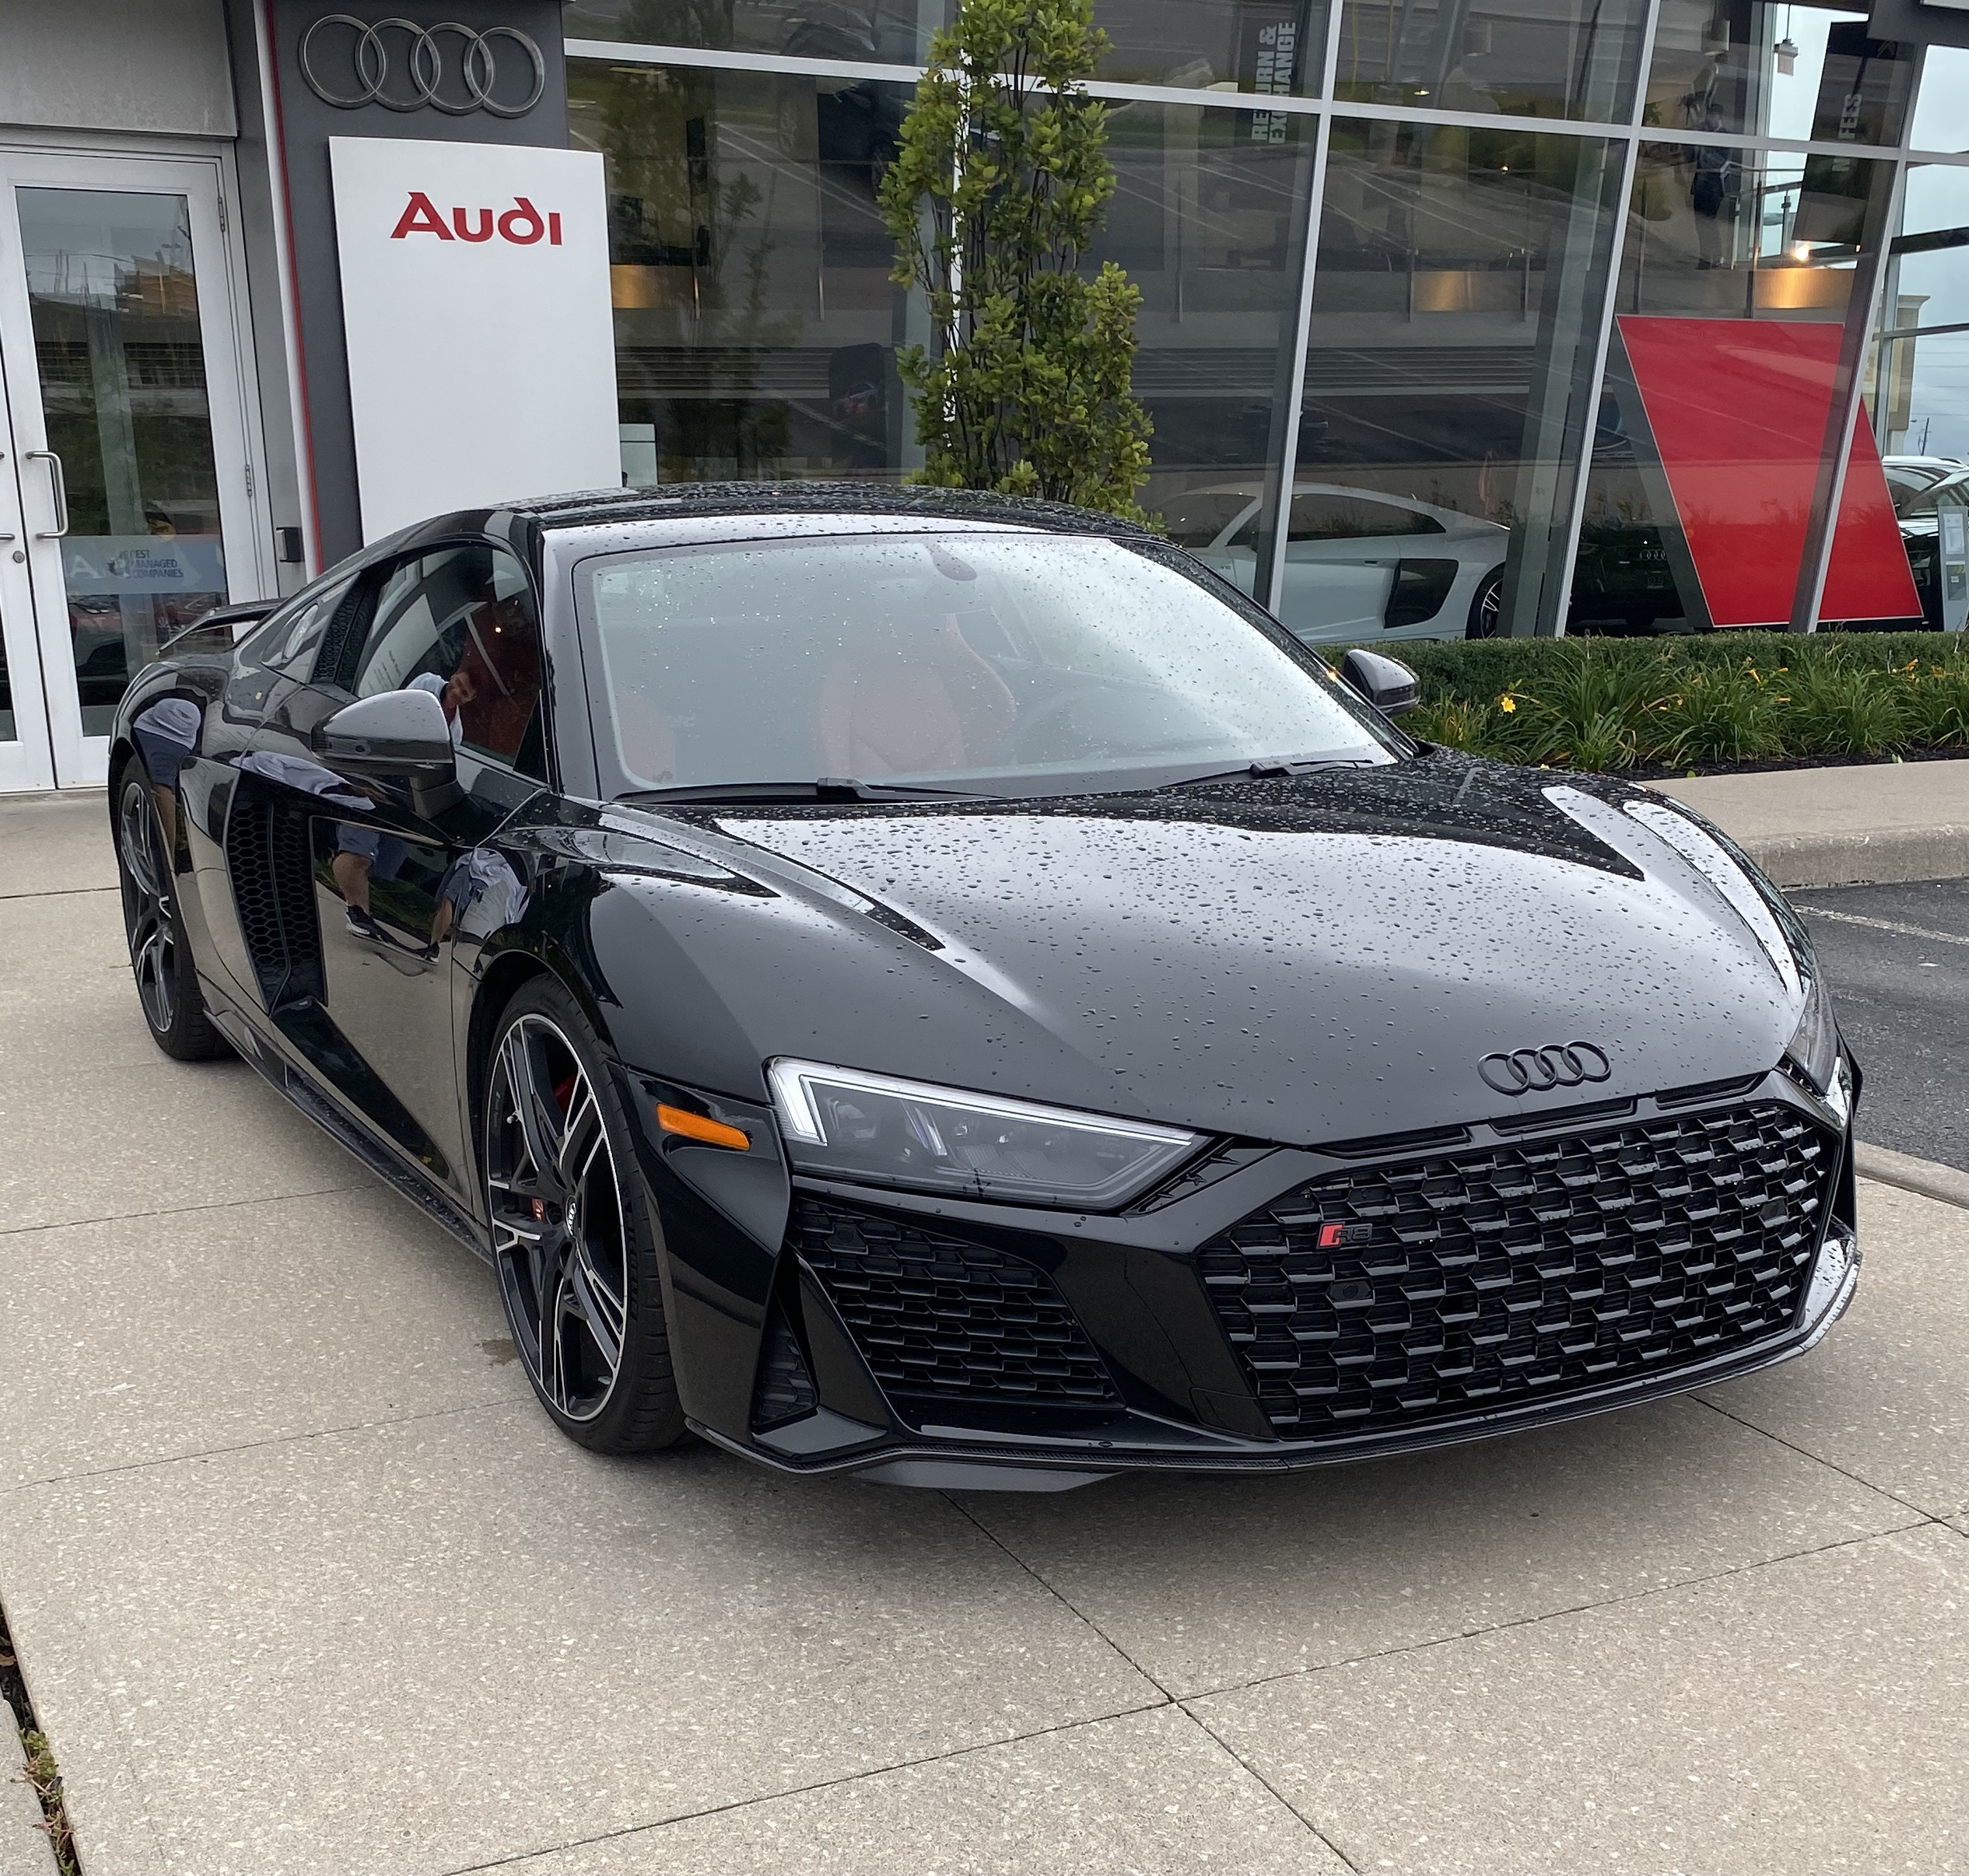
\includegraphics[width=0.5\linewidth]{images/AudiR8.jpg}
\caption{Original image}
\label{fig:Audi R8}
\end{figure}

The original image was converted into gray-scale image and applied power-law transformation with \(\gamma = 0.3\) and \(\gamma = 3\), respectively, using the following code:

\begin{lstlisting}[language=Matlab]
% Load the original image
img = imread('/lamnguyen/Desktop/School/
Computer-Vision/A1/images/AudiR8.jpg');

% Convert the image to grayscale
gray_img = rgb2gray(img);

% Perform power-law transformation on the 
% grayscale image
% Gamma equals to 0.3 
img1 = imadjust(gray_img, [], [], 0.3);

% Gamma equals to 3
img2 = imadjust(gray_img, [], [], 3);

% Display results
figure;
imshow(gray_img)

figure;
imshow(img1)

figure;
imshow(img2)
\end{lstlisting}

\begin{figure}[h!]
\centering
\begin{subfigure}[b]{0.3\linewidth}
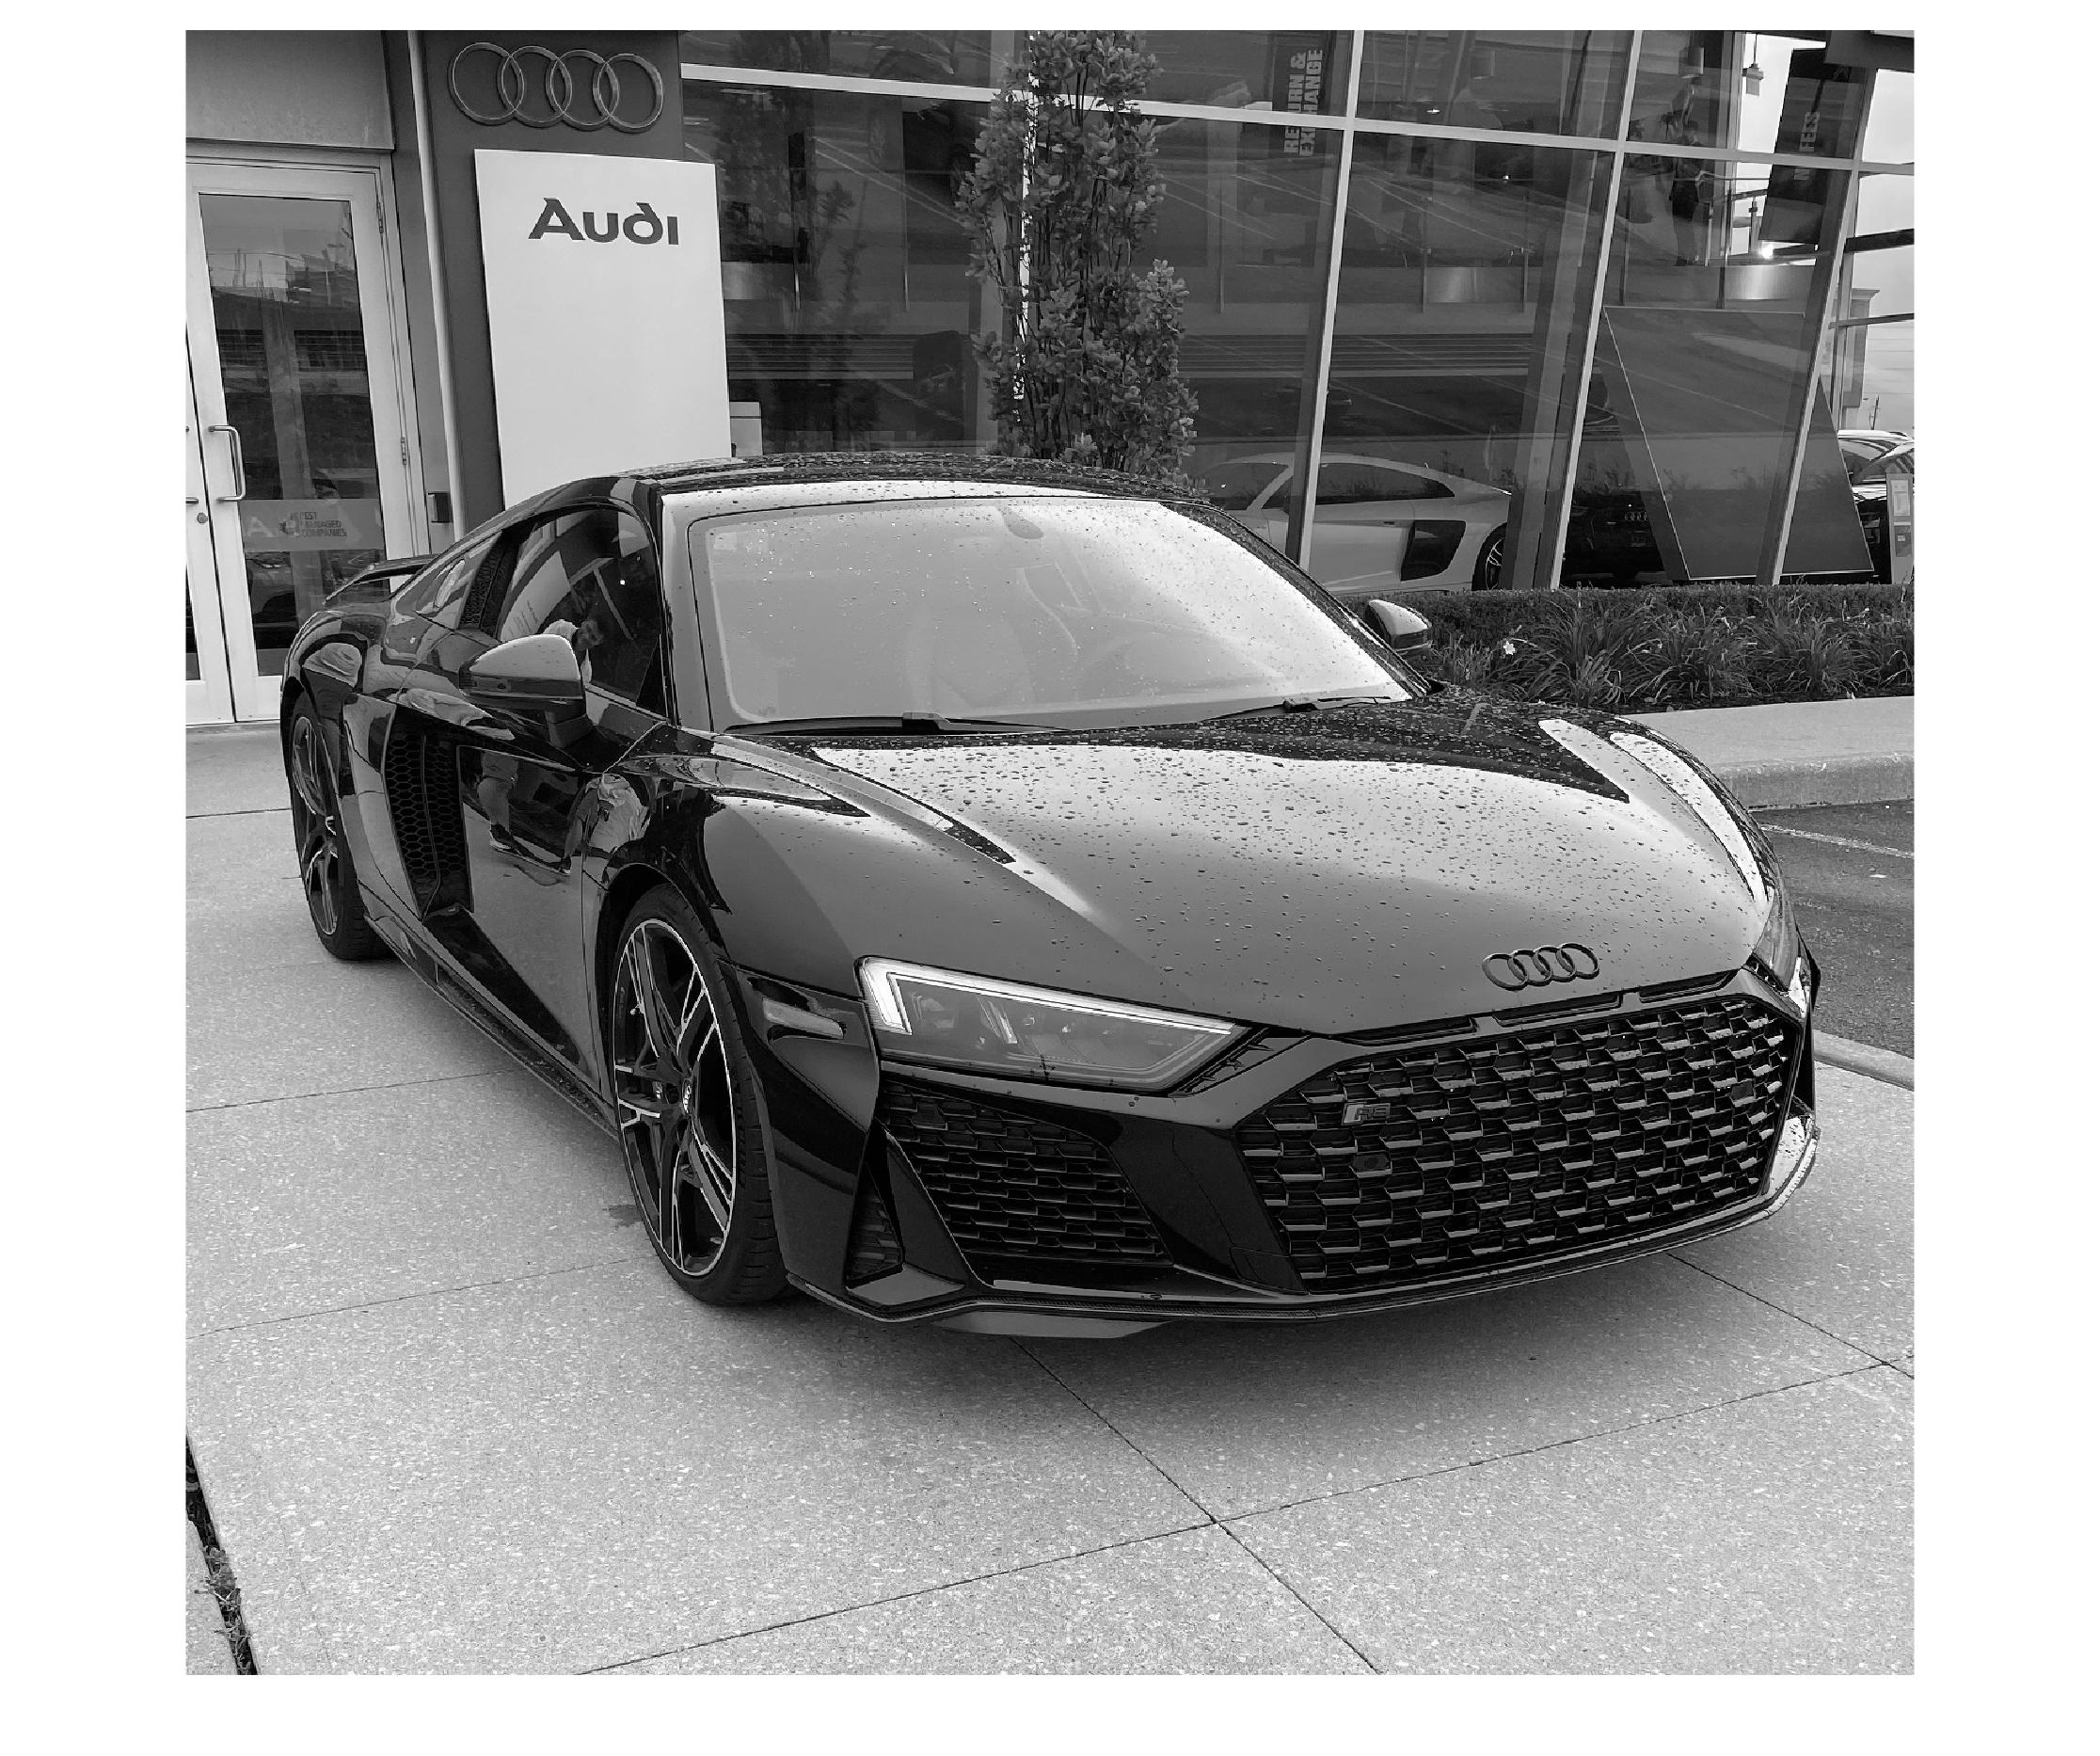
\includegraphics[width=\linewidth]{images/img1.jpg}
\caption{Grayscale}
\end{subfigure}
\begin{subfigure}[b]{0.3\linewidth}
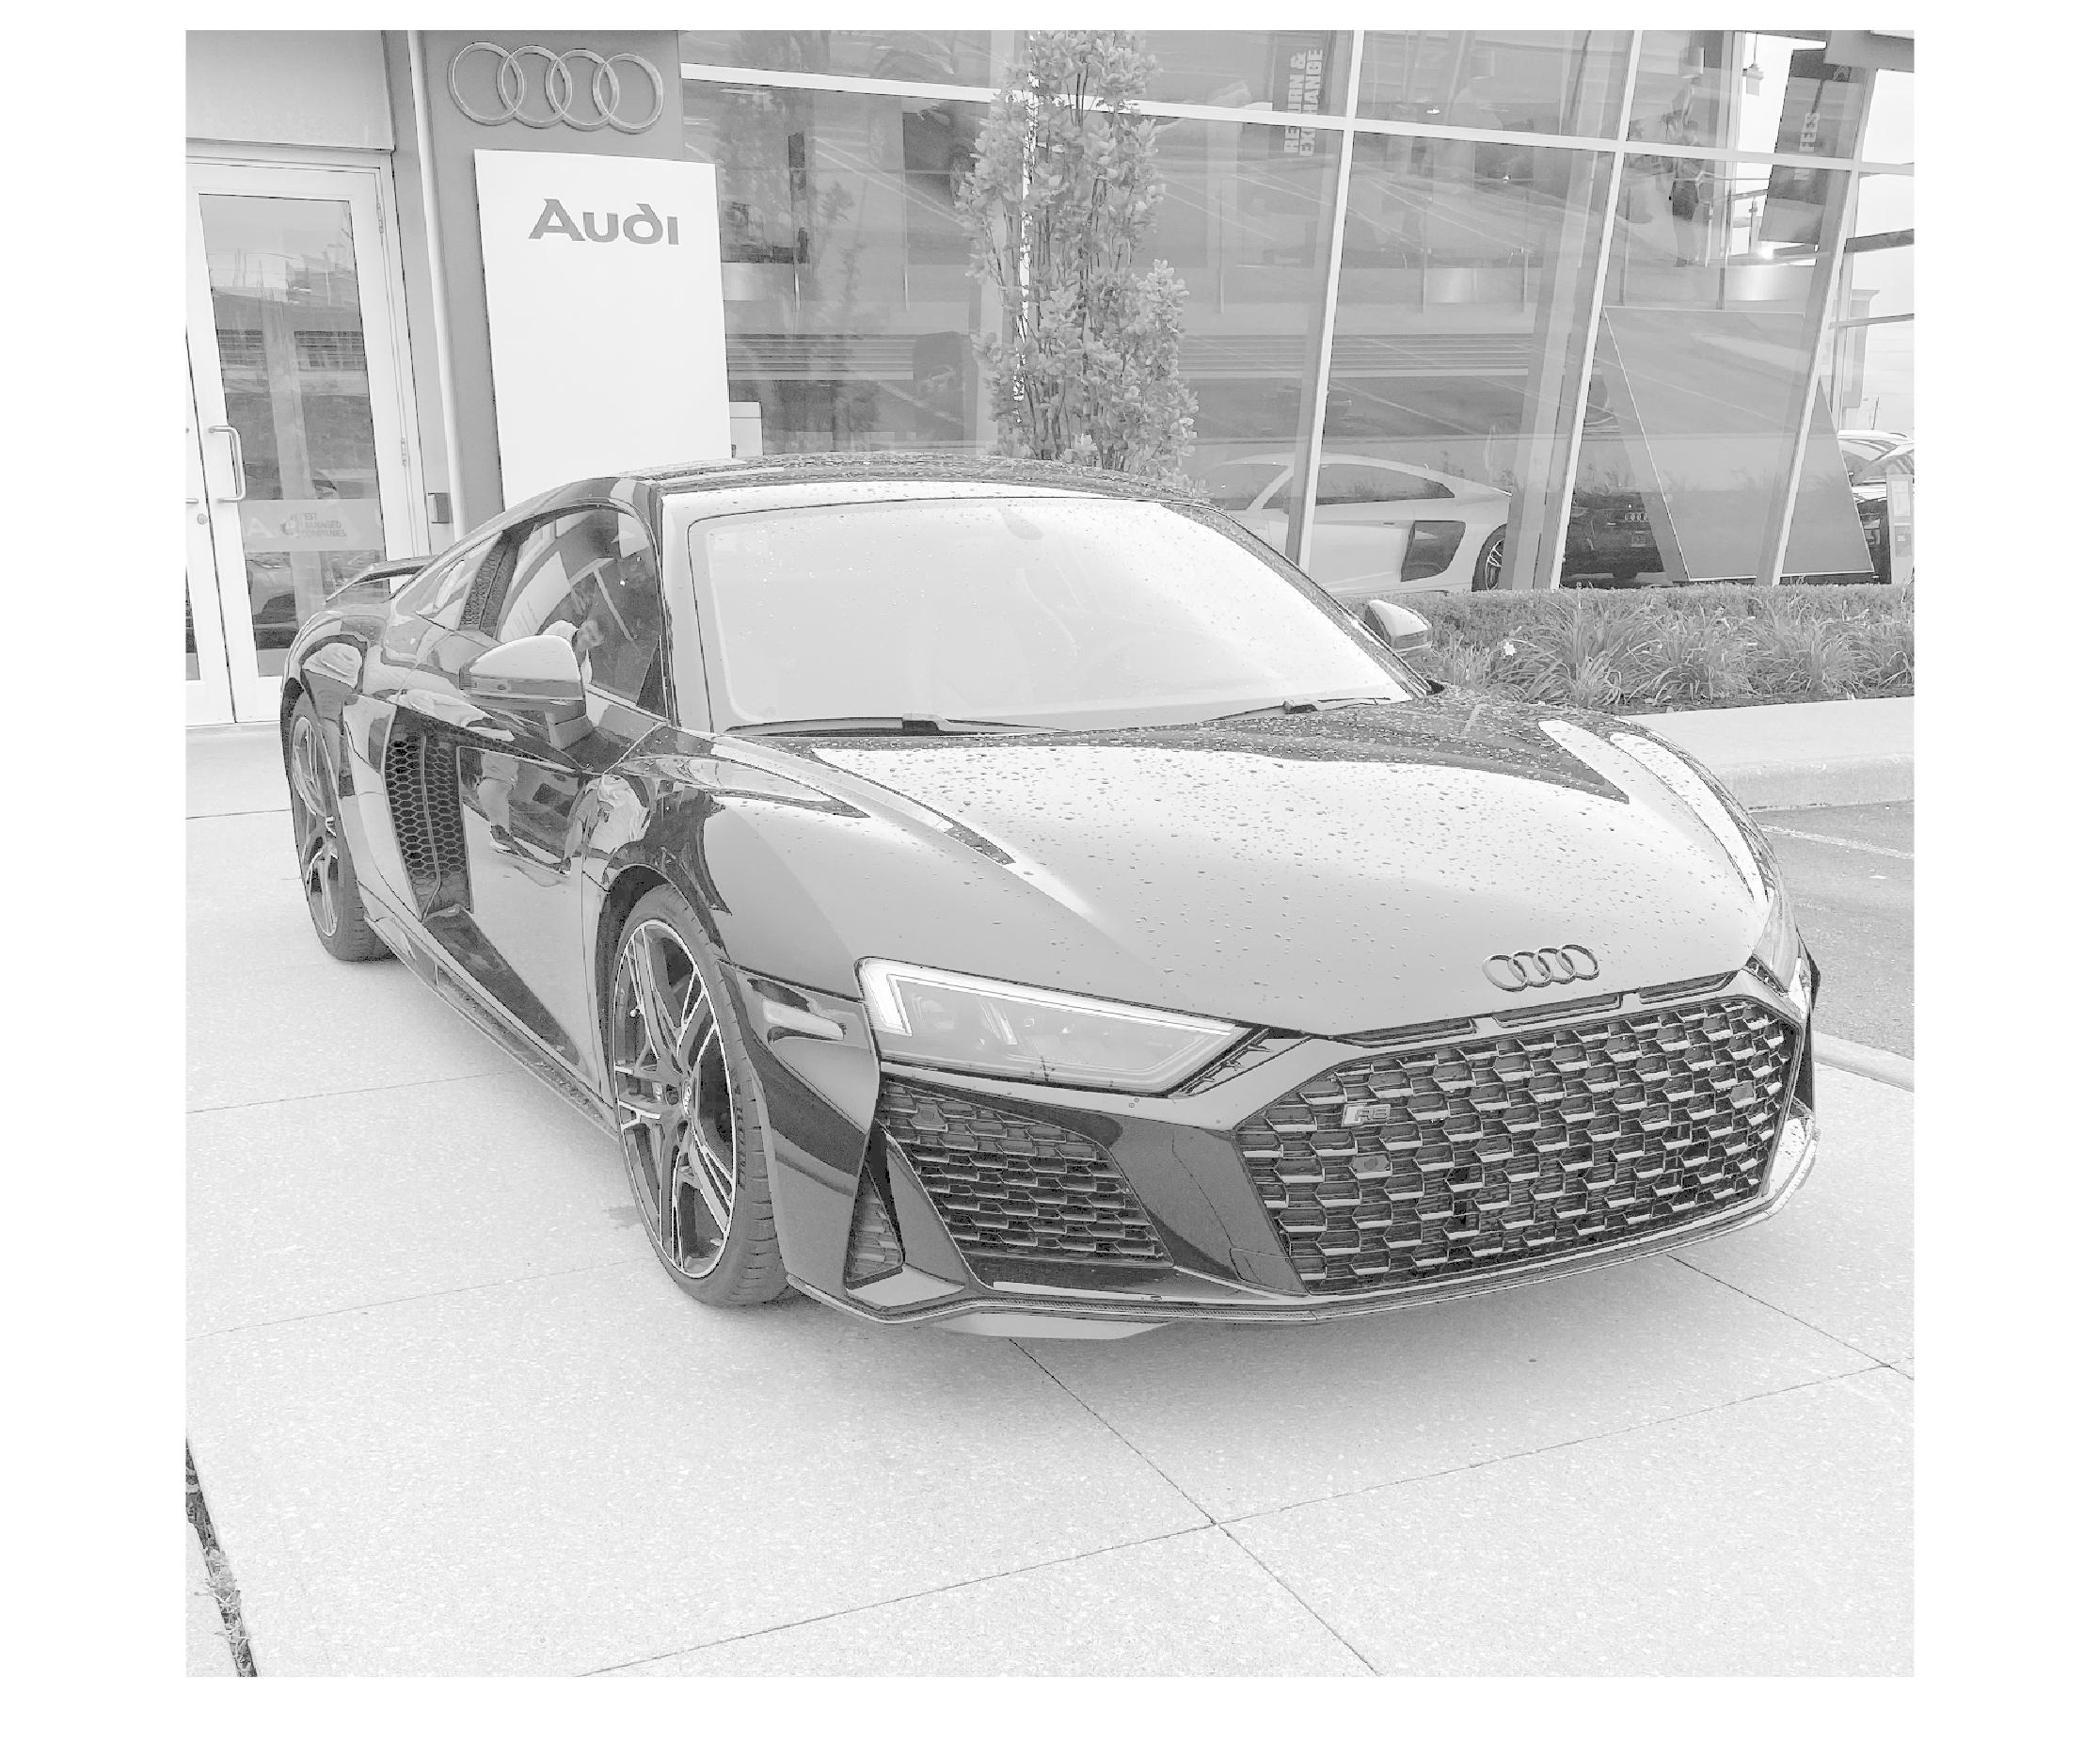
\includegraphics[width=\linewidth]{images/img2.jpg}
\caption{\(\gamma = 0.3\)}
\end{subfigure}
\begin{subfigure}[b]{0.3\linewidth}
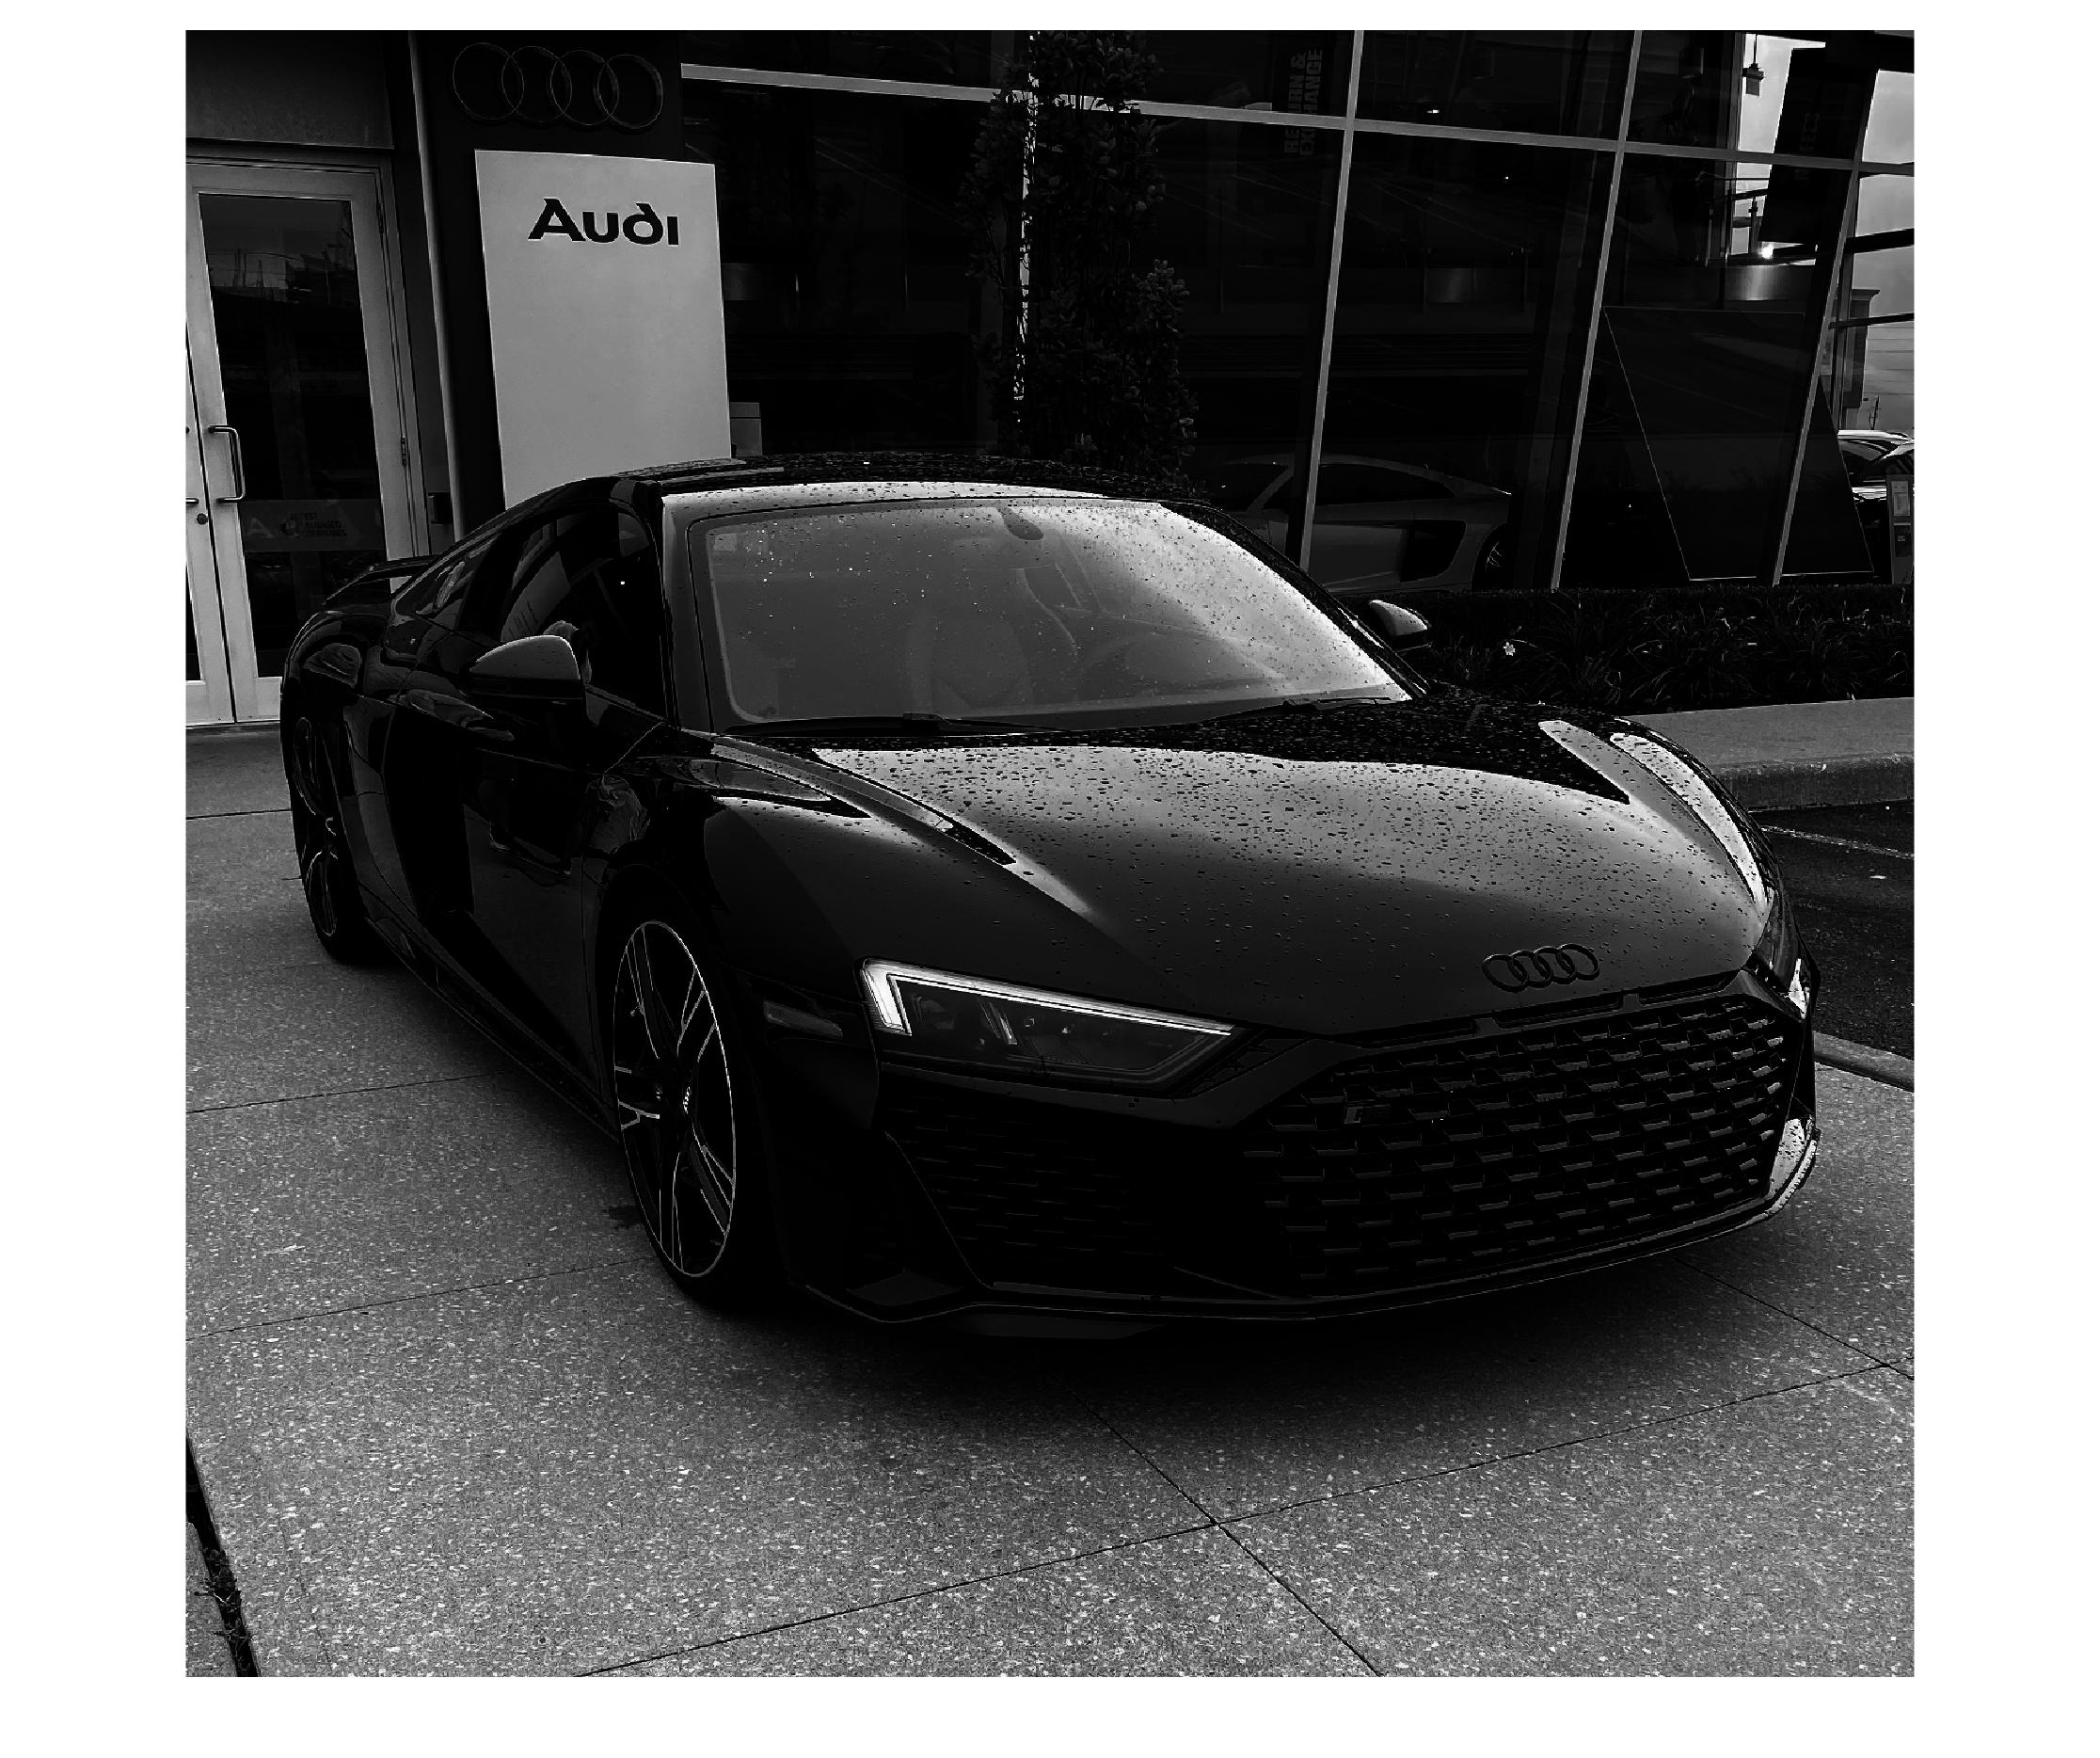
\includegraphics[width=\linewidth]{images/img3.jpg}
\caption{\(\gamma = 3\)}
\end{subfigure}
\caption{Power-law transformation results}
\label{fig:power-law transformation}
\end{figure}

As can be observed from the outputs, \(\gamma > 1\) decreases the the intensity of pixels which makes the images darker. On the other hand, \(\gamma < 1\) increases the the intensity of pixels which makes the images lighter.

\newpage

\subsection{Problem 2}

The 8 bit-plane slicing technique is performed on the grayscale image as follow: 

\begin{lstlisting}[language=Matlab]

% Load the original image
img=imread('/lamnguyen/Desktop/School
/Computer-Vision/A1/images/AudiR8.jpg');

% Convert the image to grayscale
gray_img = rgb2gray(img);

% Extract bit-plane
%Extract 1st bit-plane
b1 = bitget(gray_img,1); 
%Extract 2nd bit-plane
b2 = bitget(gray_img,2); 
%Extract 3rd bit-plane
b3 = bitget(gray_img,3); 
%Extract 4th bit-plane
b4 = bitget(gray_img,4); 
%Extract 5th bit-plane
b5 = bitget(gray_img,5); 
%Extract 6th bit-plane
b6 = bitget(gray_img,6); 
%Extract 7th bit-plane
b7 = bitget(gray_img,7); 
%Extract 8th bit-plane
b8 = bitget(gray_img,8);

% Show 8 bit-plane slicing results
figure;
imshow(b1*255)
figure;
imshow(b2*255)
figure;
imshow(b3*255)
figure;
imshow(b4*255)
figure;
imshow(b5*255)
figure;
imshow(b6*255)
figure;
imshow(b7*255)
figure; 
imshow(b8*255)

\end{lstlisting}

For an 8-bit image, 0 is encoded as 00000000 and 255 is encoded as 11111111. Any number between 0 to 255 is encoded as one byte. The 8\textsuperscript{th} bit-plane is referred as the most significant bit (MSB) because a change in that bit would significantly change the value encoded by the byte. The 1\textsuperscript{st} bit-plane is referred as the least significant bit (LSB), because a change in this bit does not change the encoded gray value much.

\begin{figure}[h!]
\centering
\begin{subfigure}[b]{0.3\linewidth}
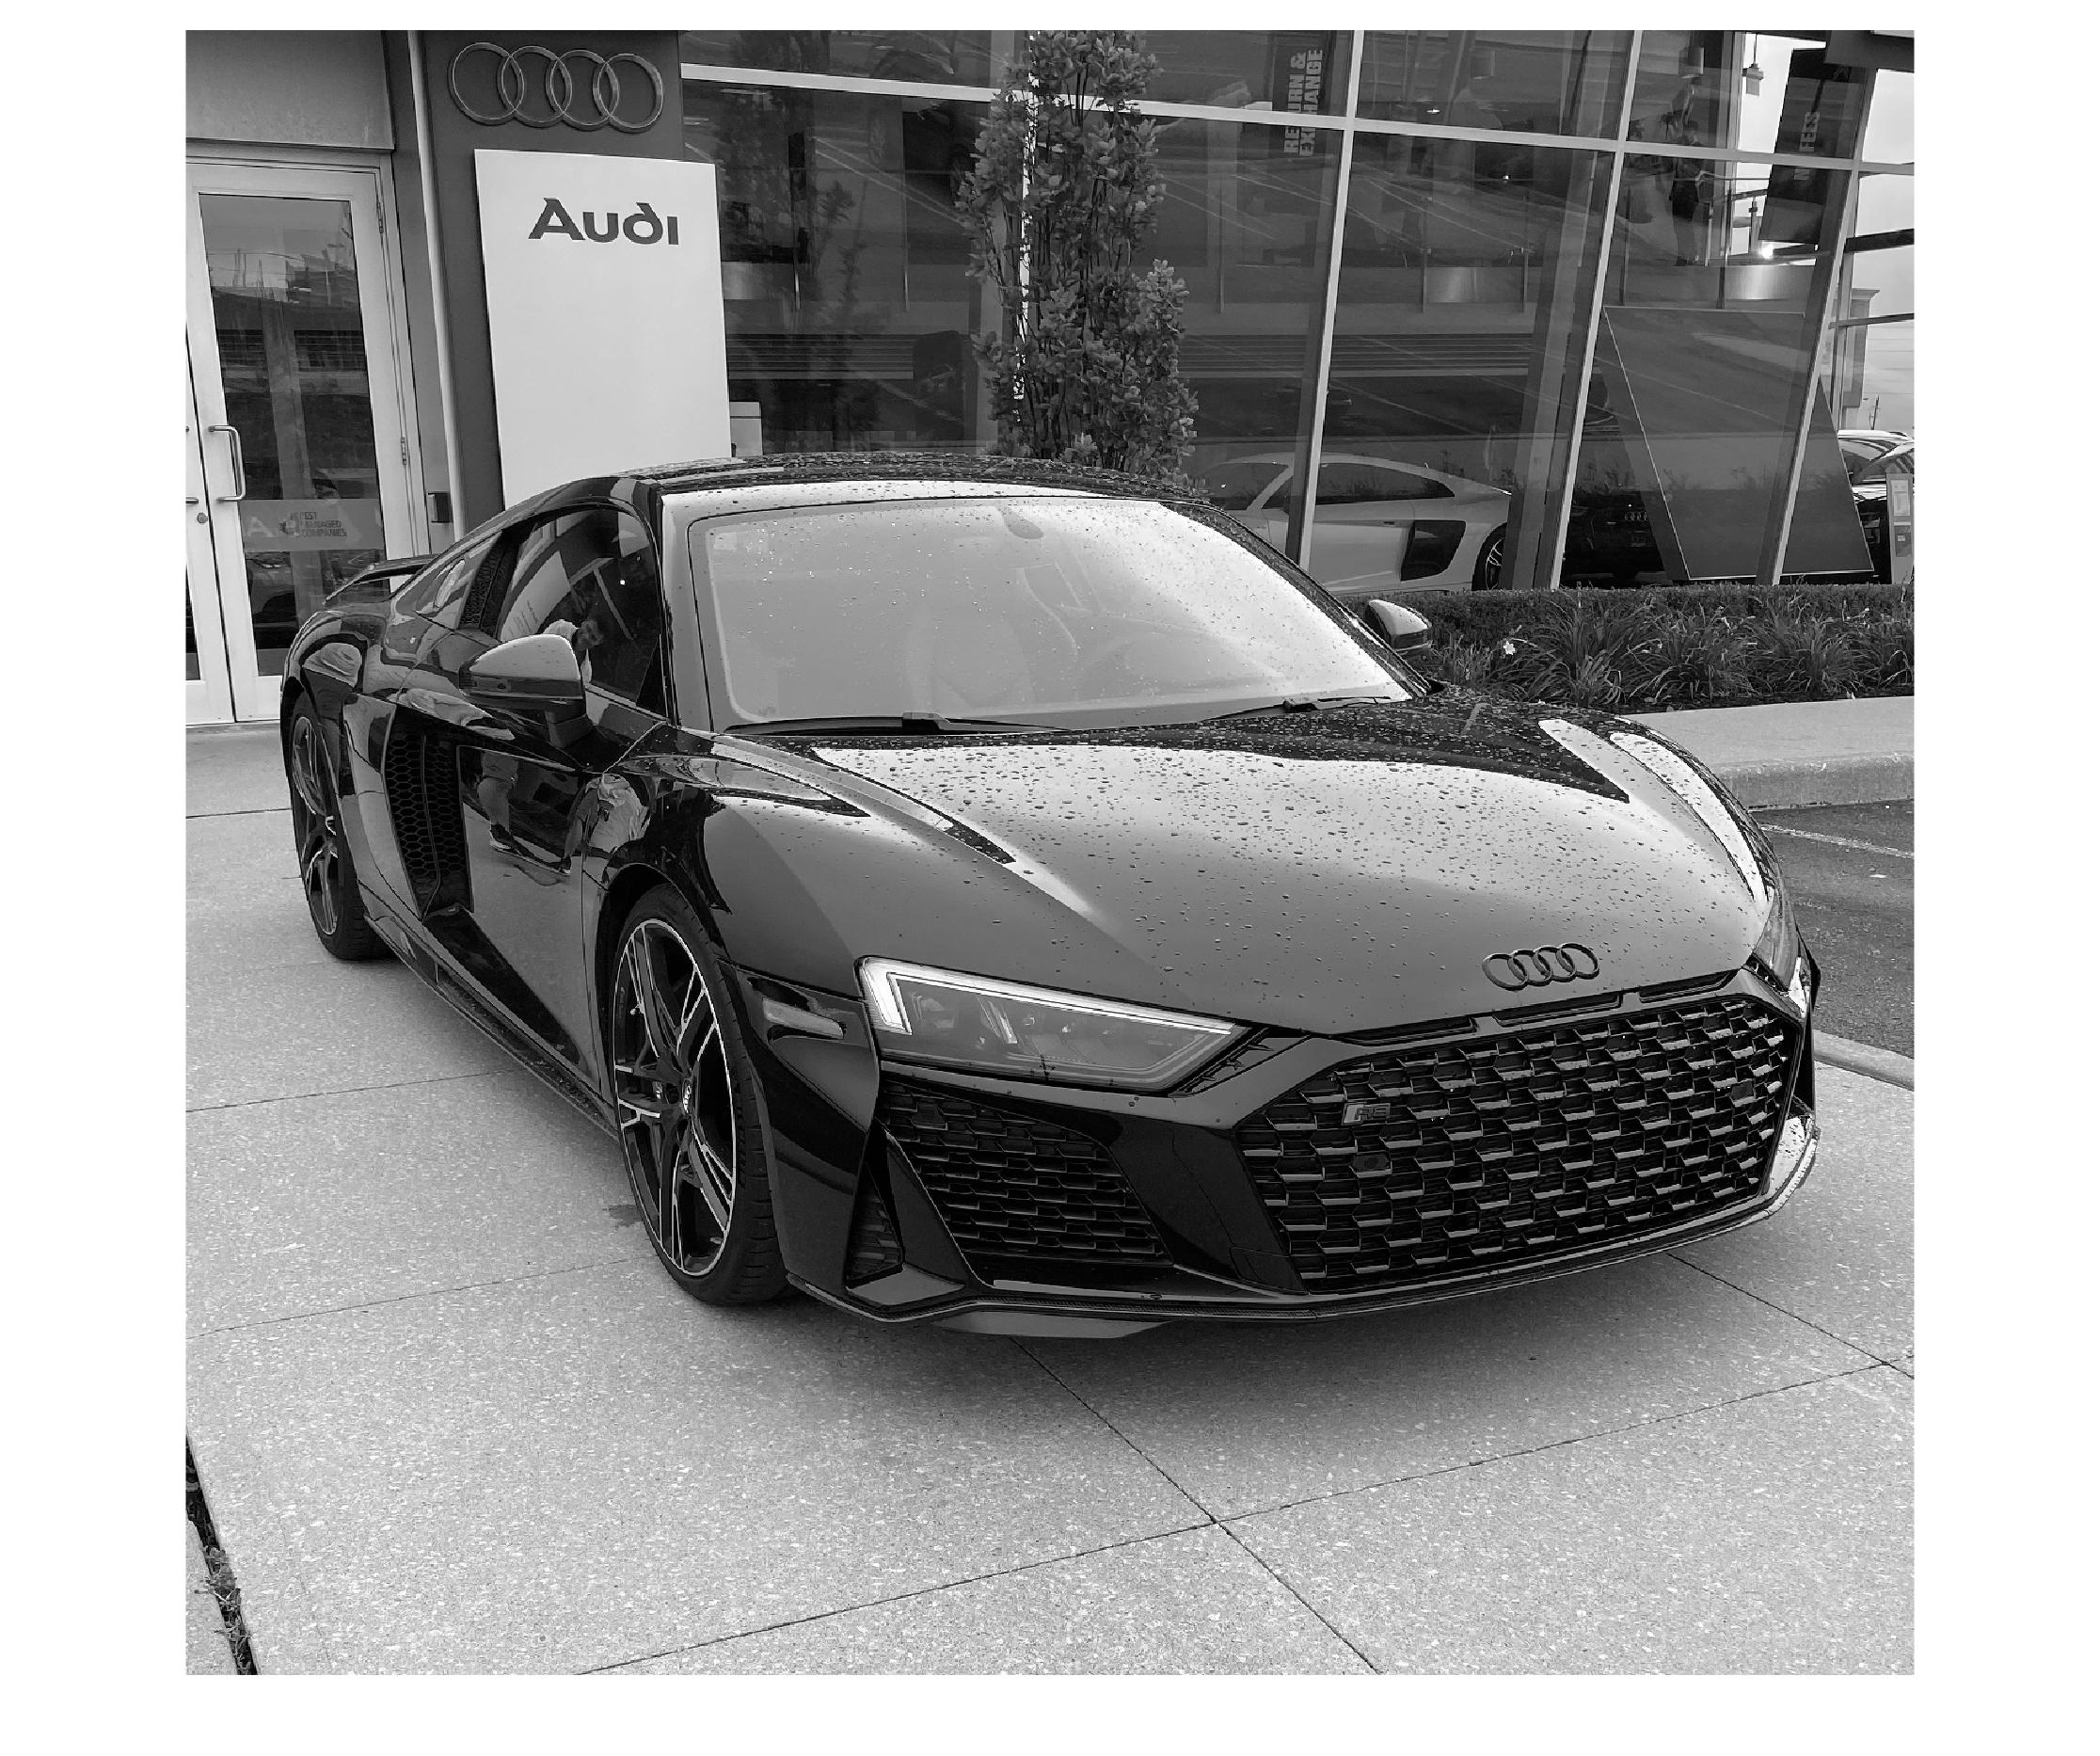
\includegraphics[width=\linewidth]{images/img1.jpg}
\caption{Grayscale}
\end{subfigure}
\begin{subfigure}[b]{0.3\linewidth}
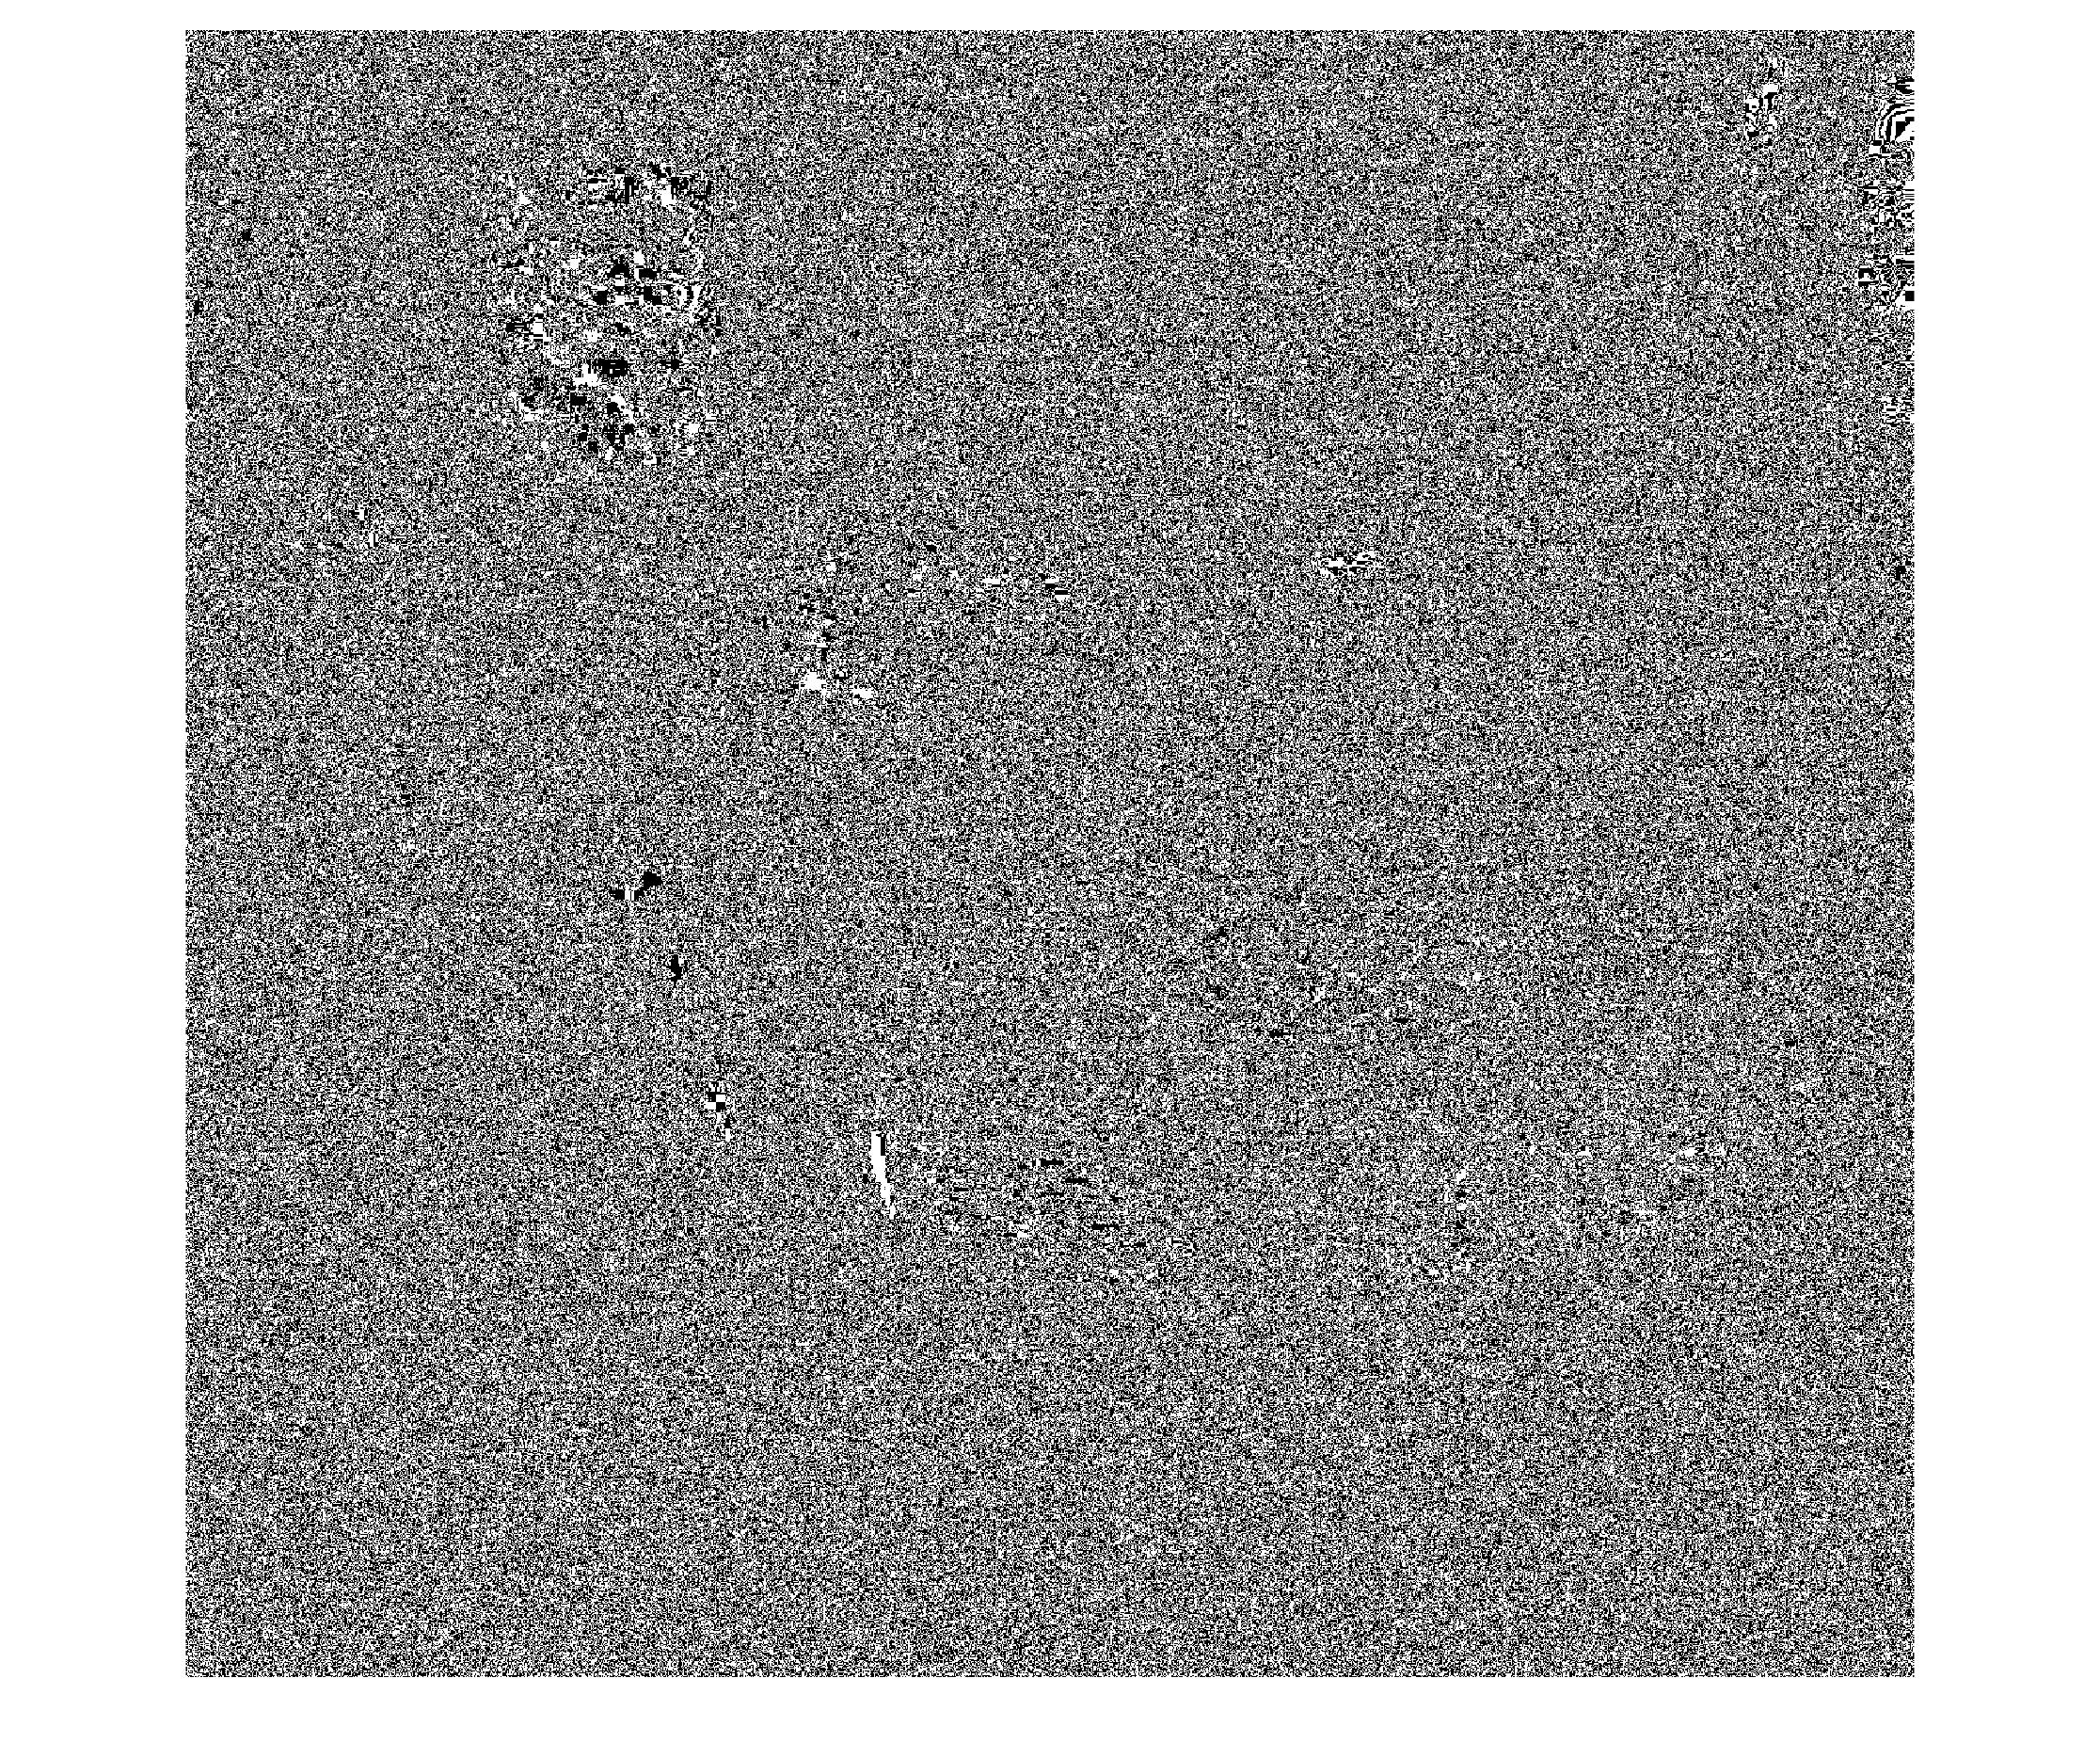
\includegraphics[width=\linewidth]{images/img4.jpg}
\caption{1\textsuperscript{st} bit-plane}
\end{subfigure}
\begin{subfigure}[b]{0.3\linewidth}
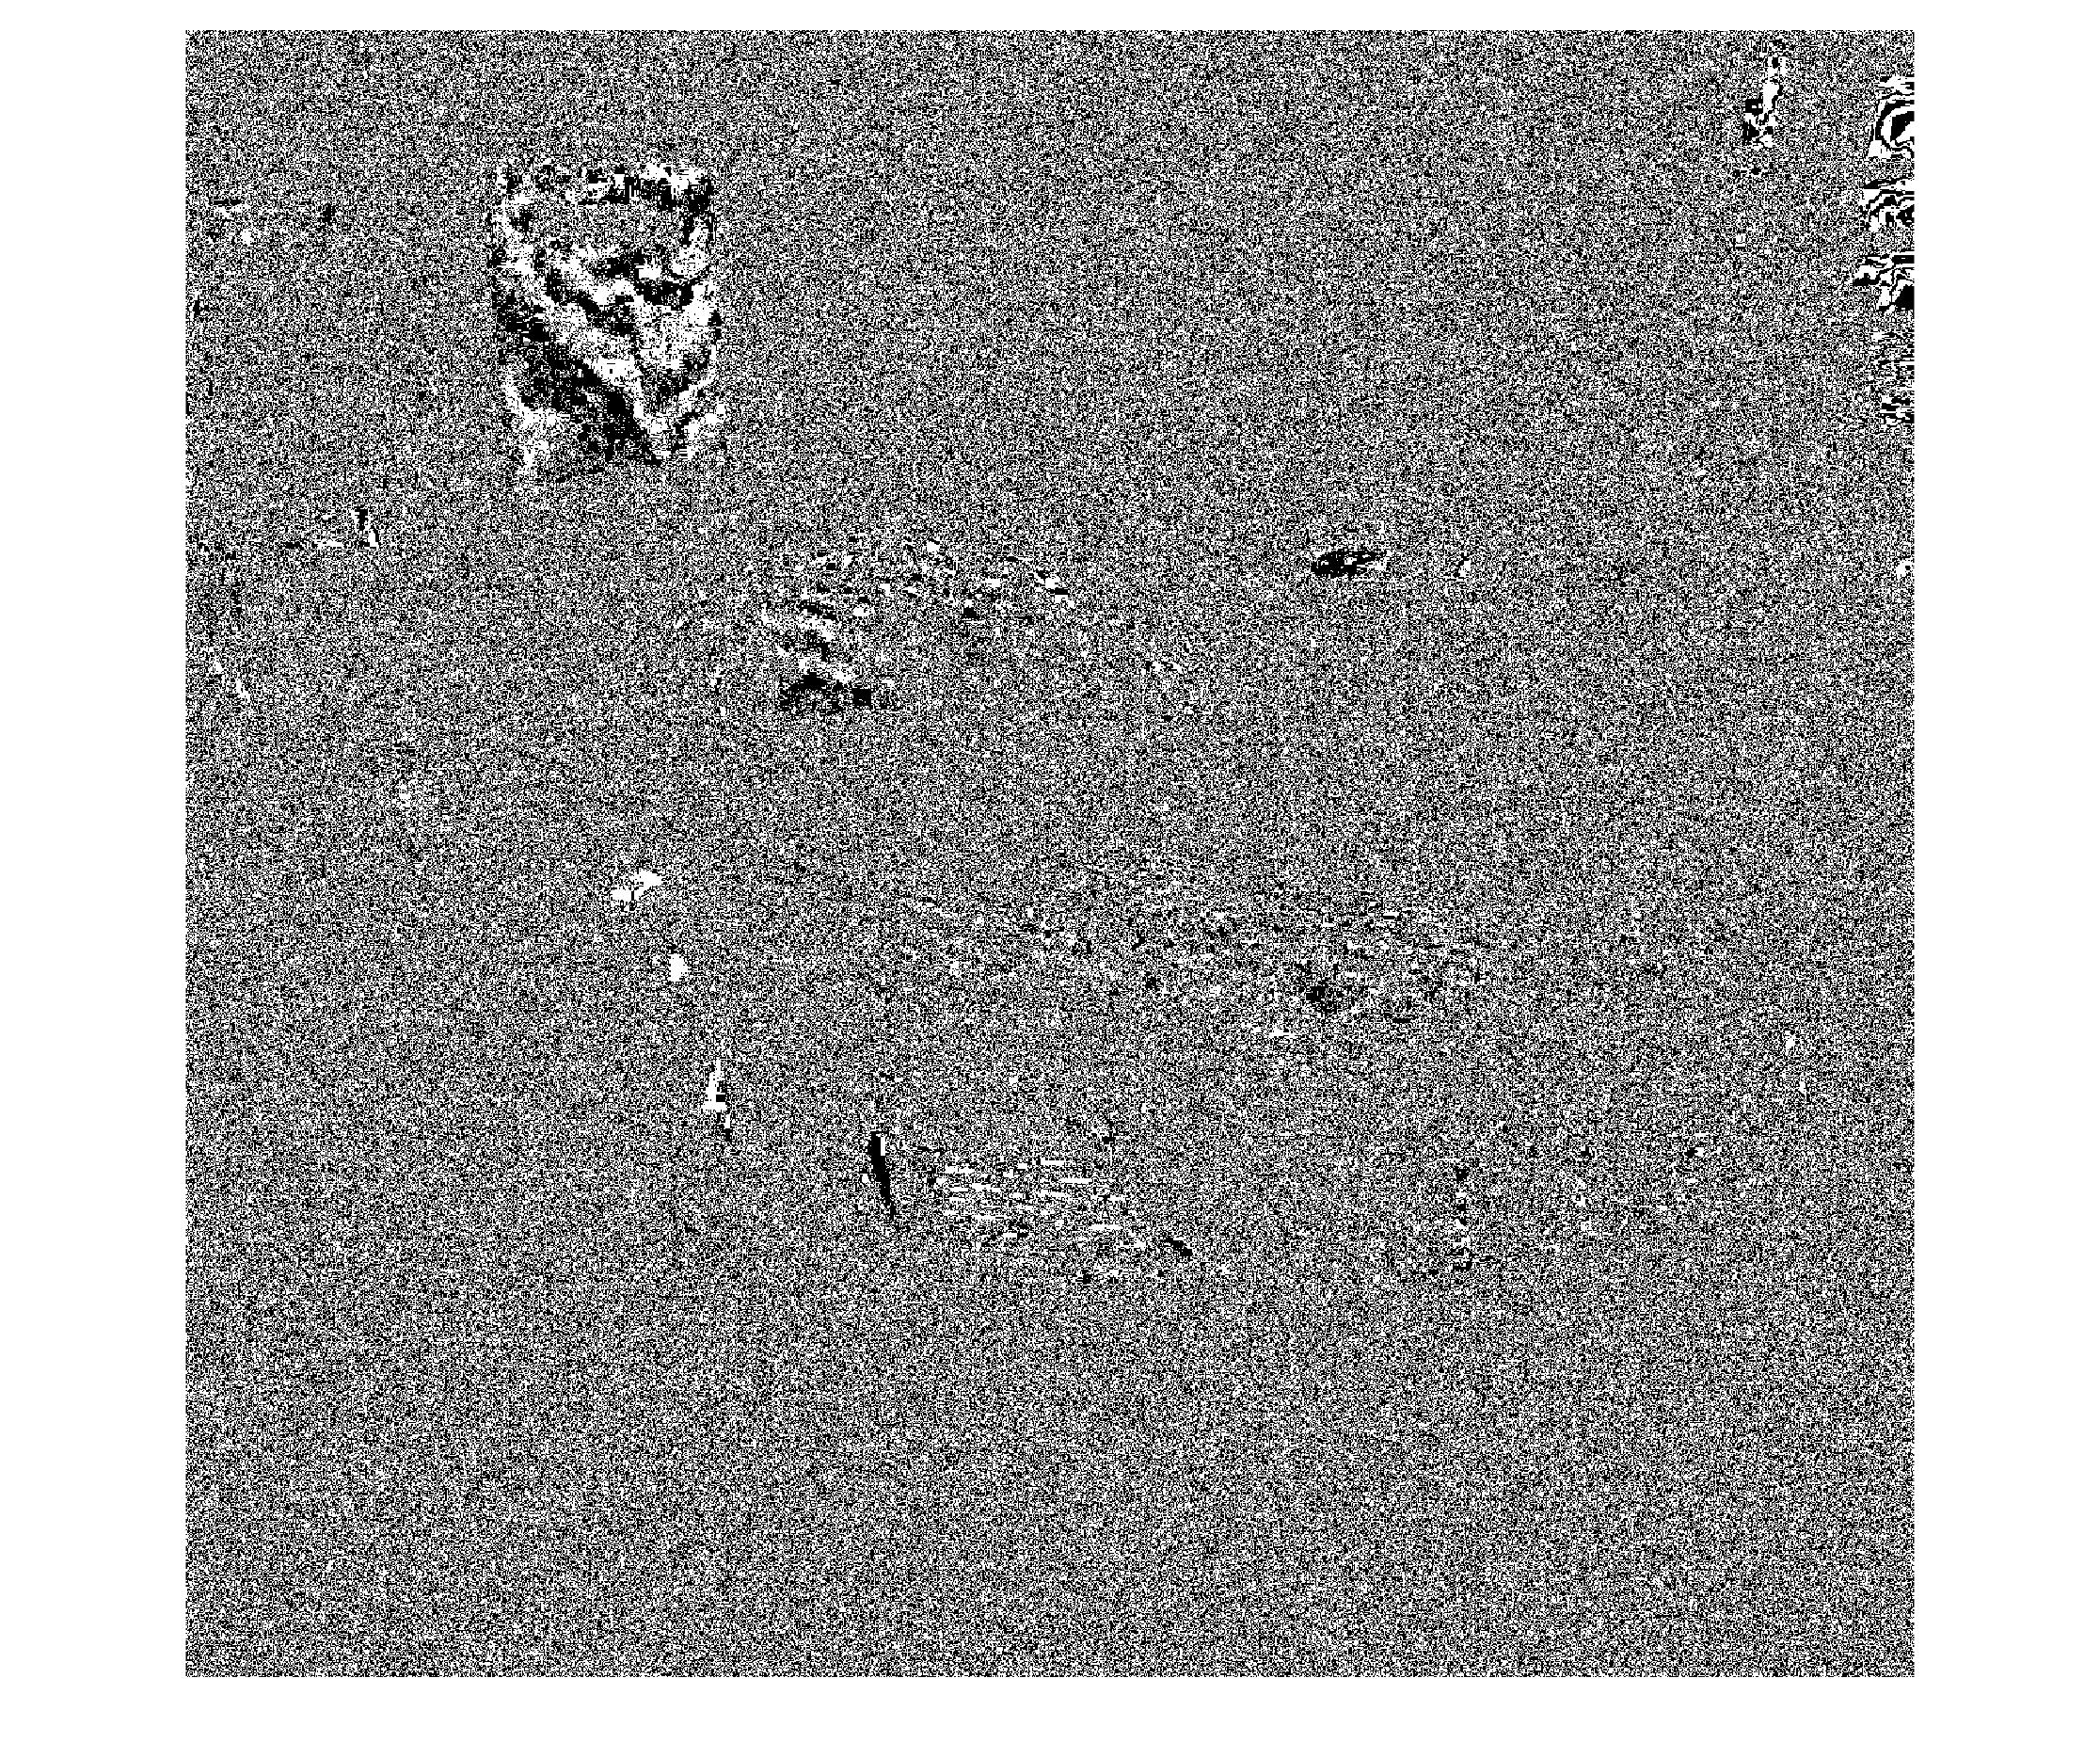
\includegraphics[width=\linewidth]{images/img5.jpg}
\caption{2\textsuperscript{nd} bit-plane}
\end{subfigure}
\begin{subfigure}[b]{0.3\linewidth}
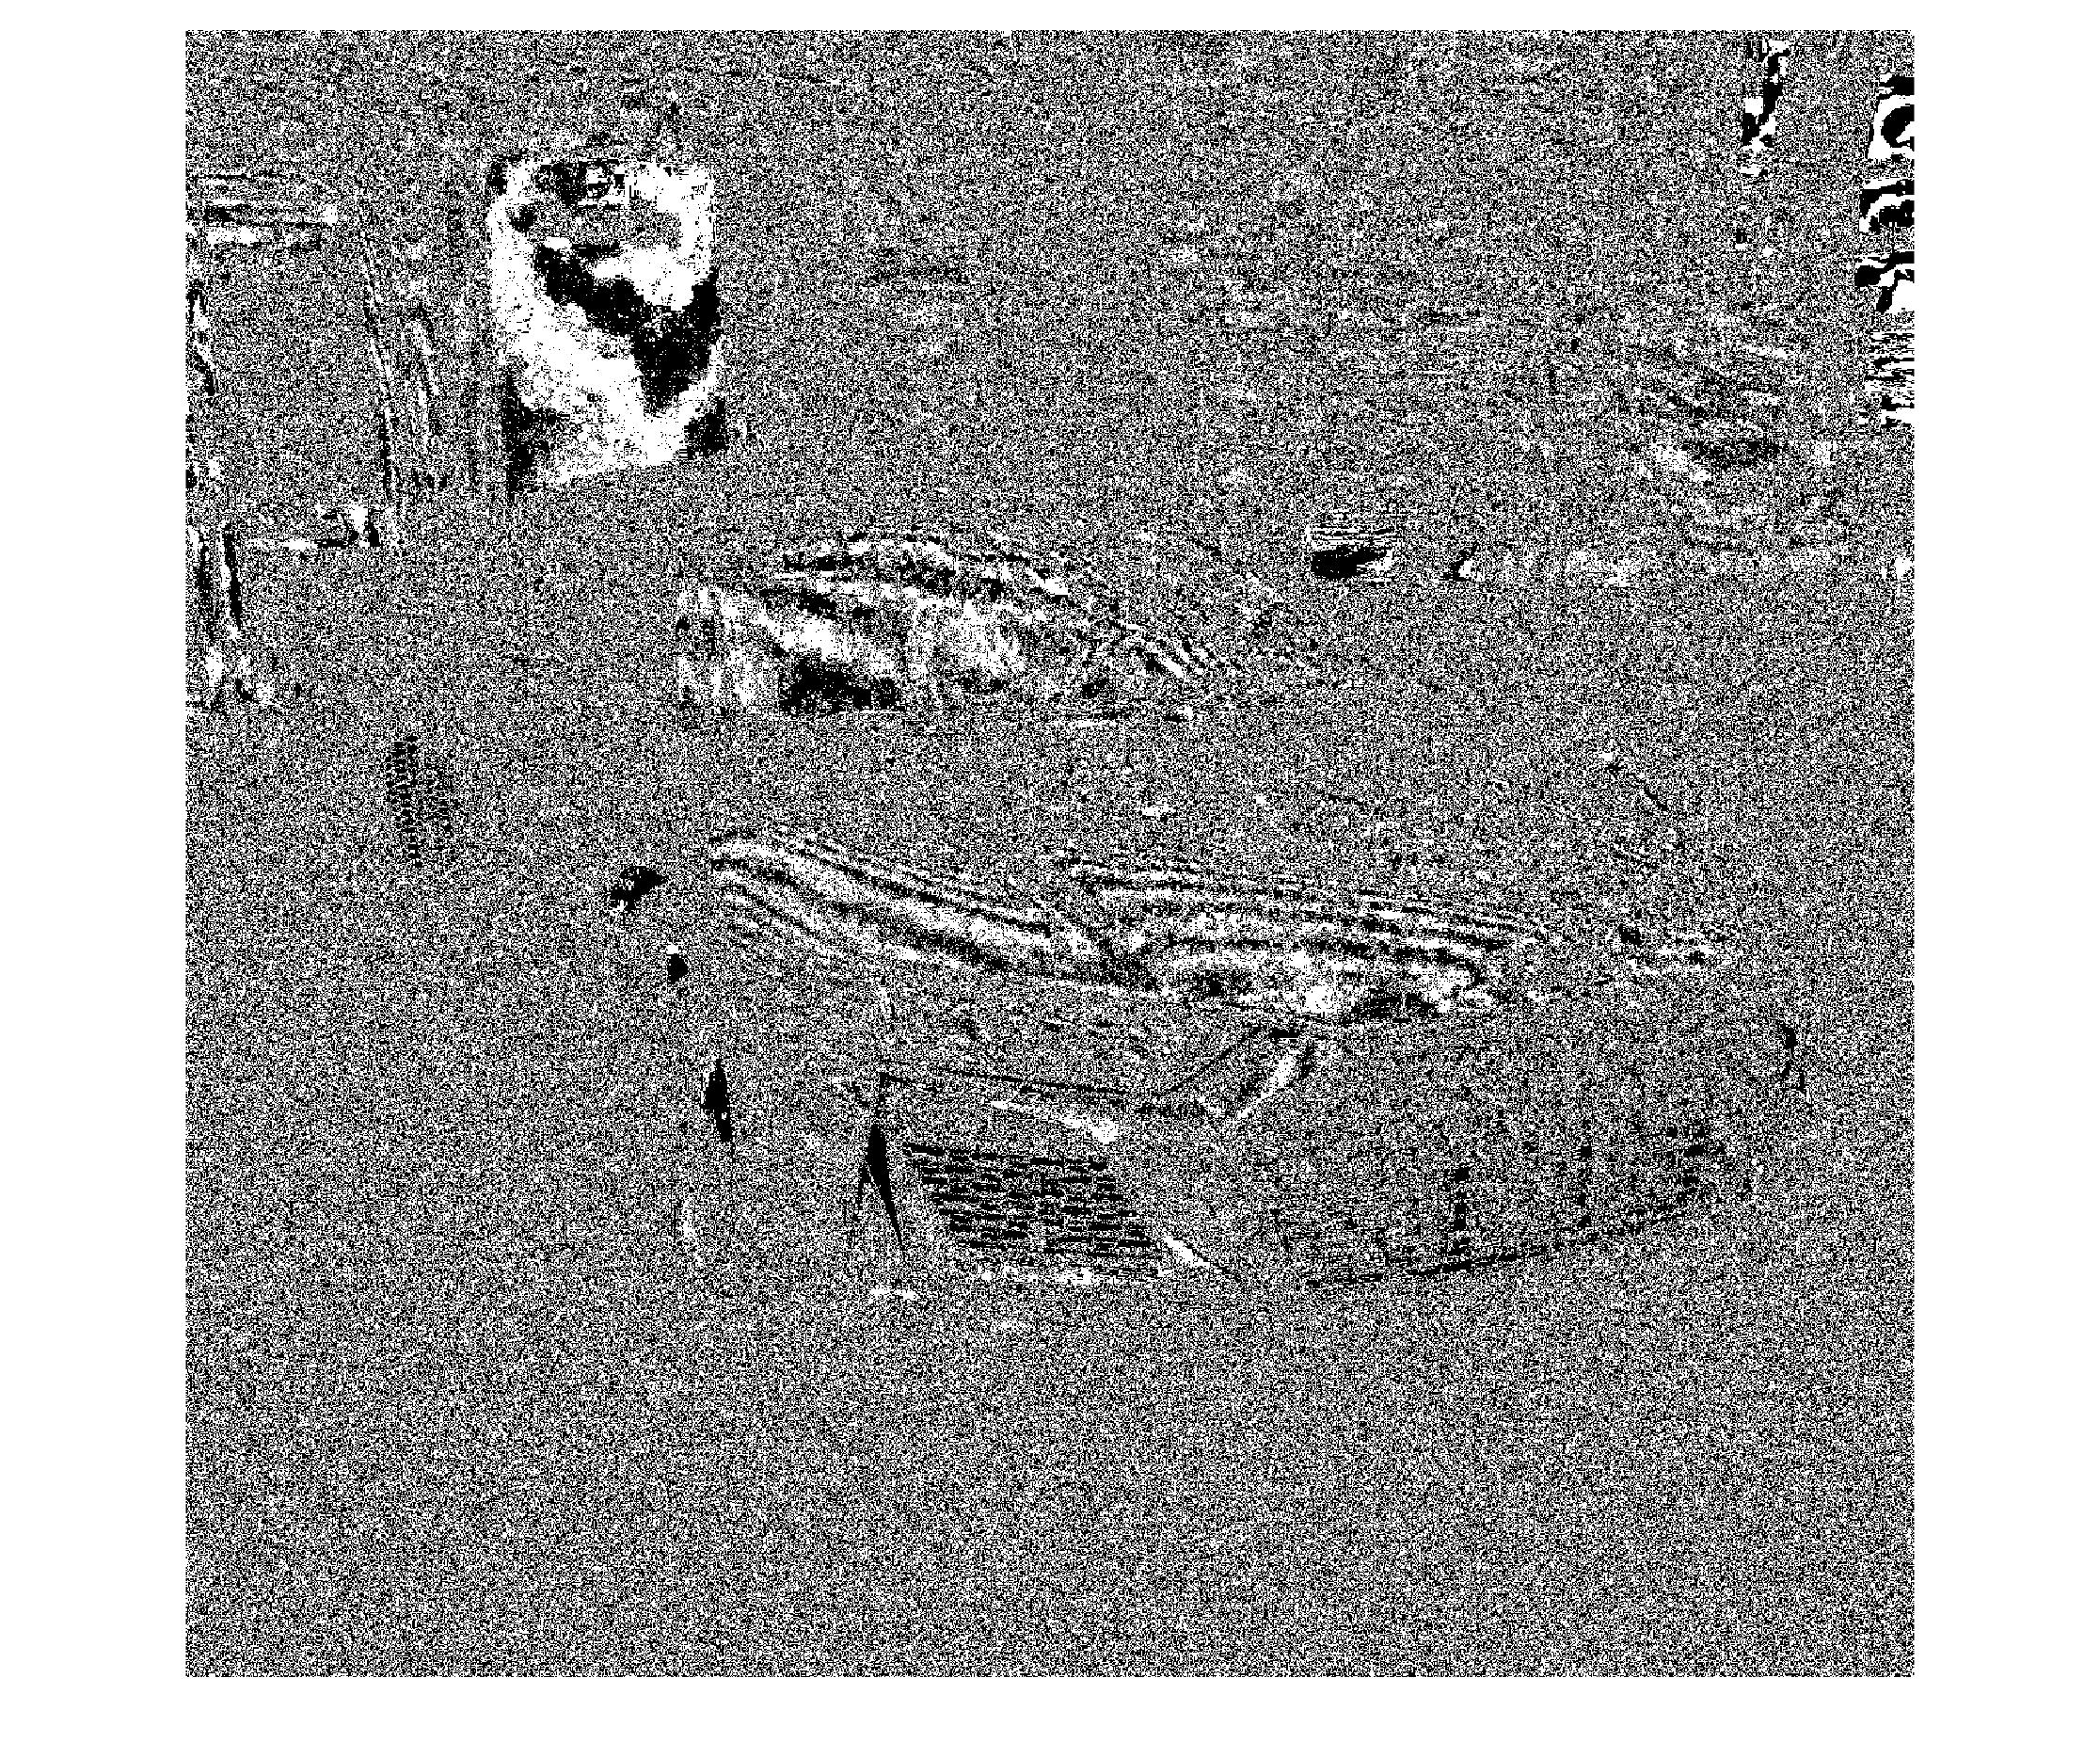
\includegraphics[width=\linewidth]{images/img6.jpg}
\caption{3\textsuperscript{rd} bit-plane}
\end{subfigure}
\begin{subfigure}[b]{0.3\linewidth}
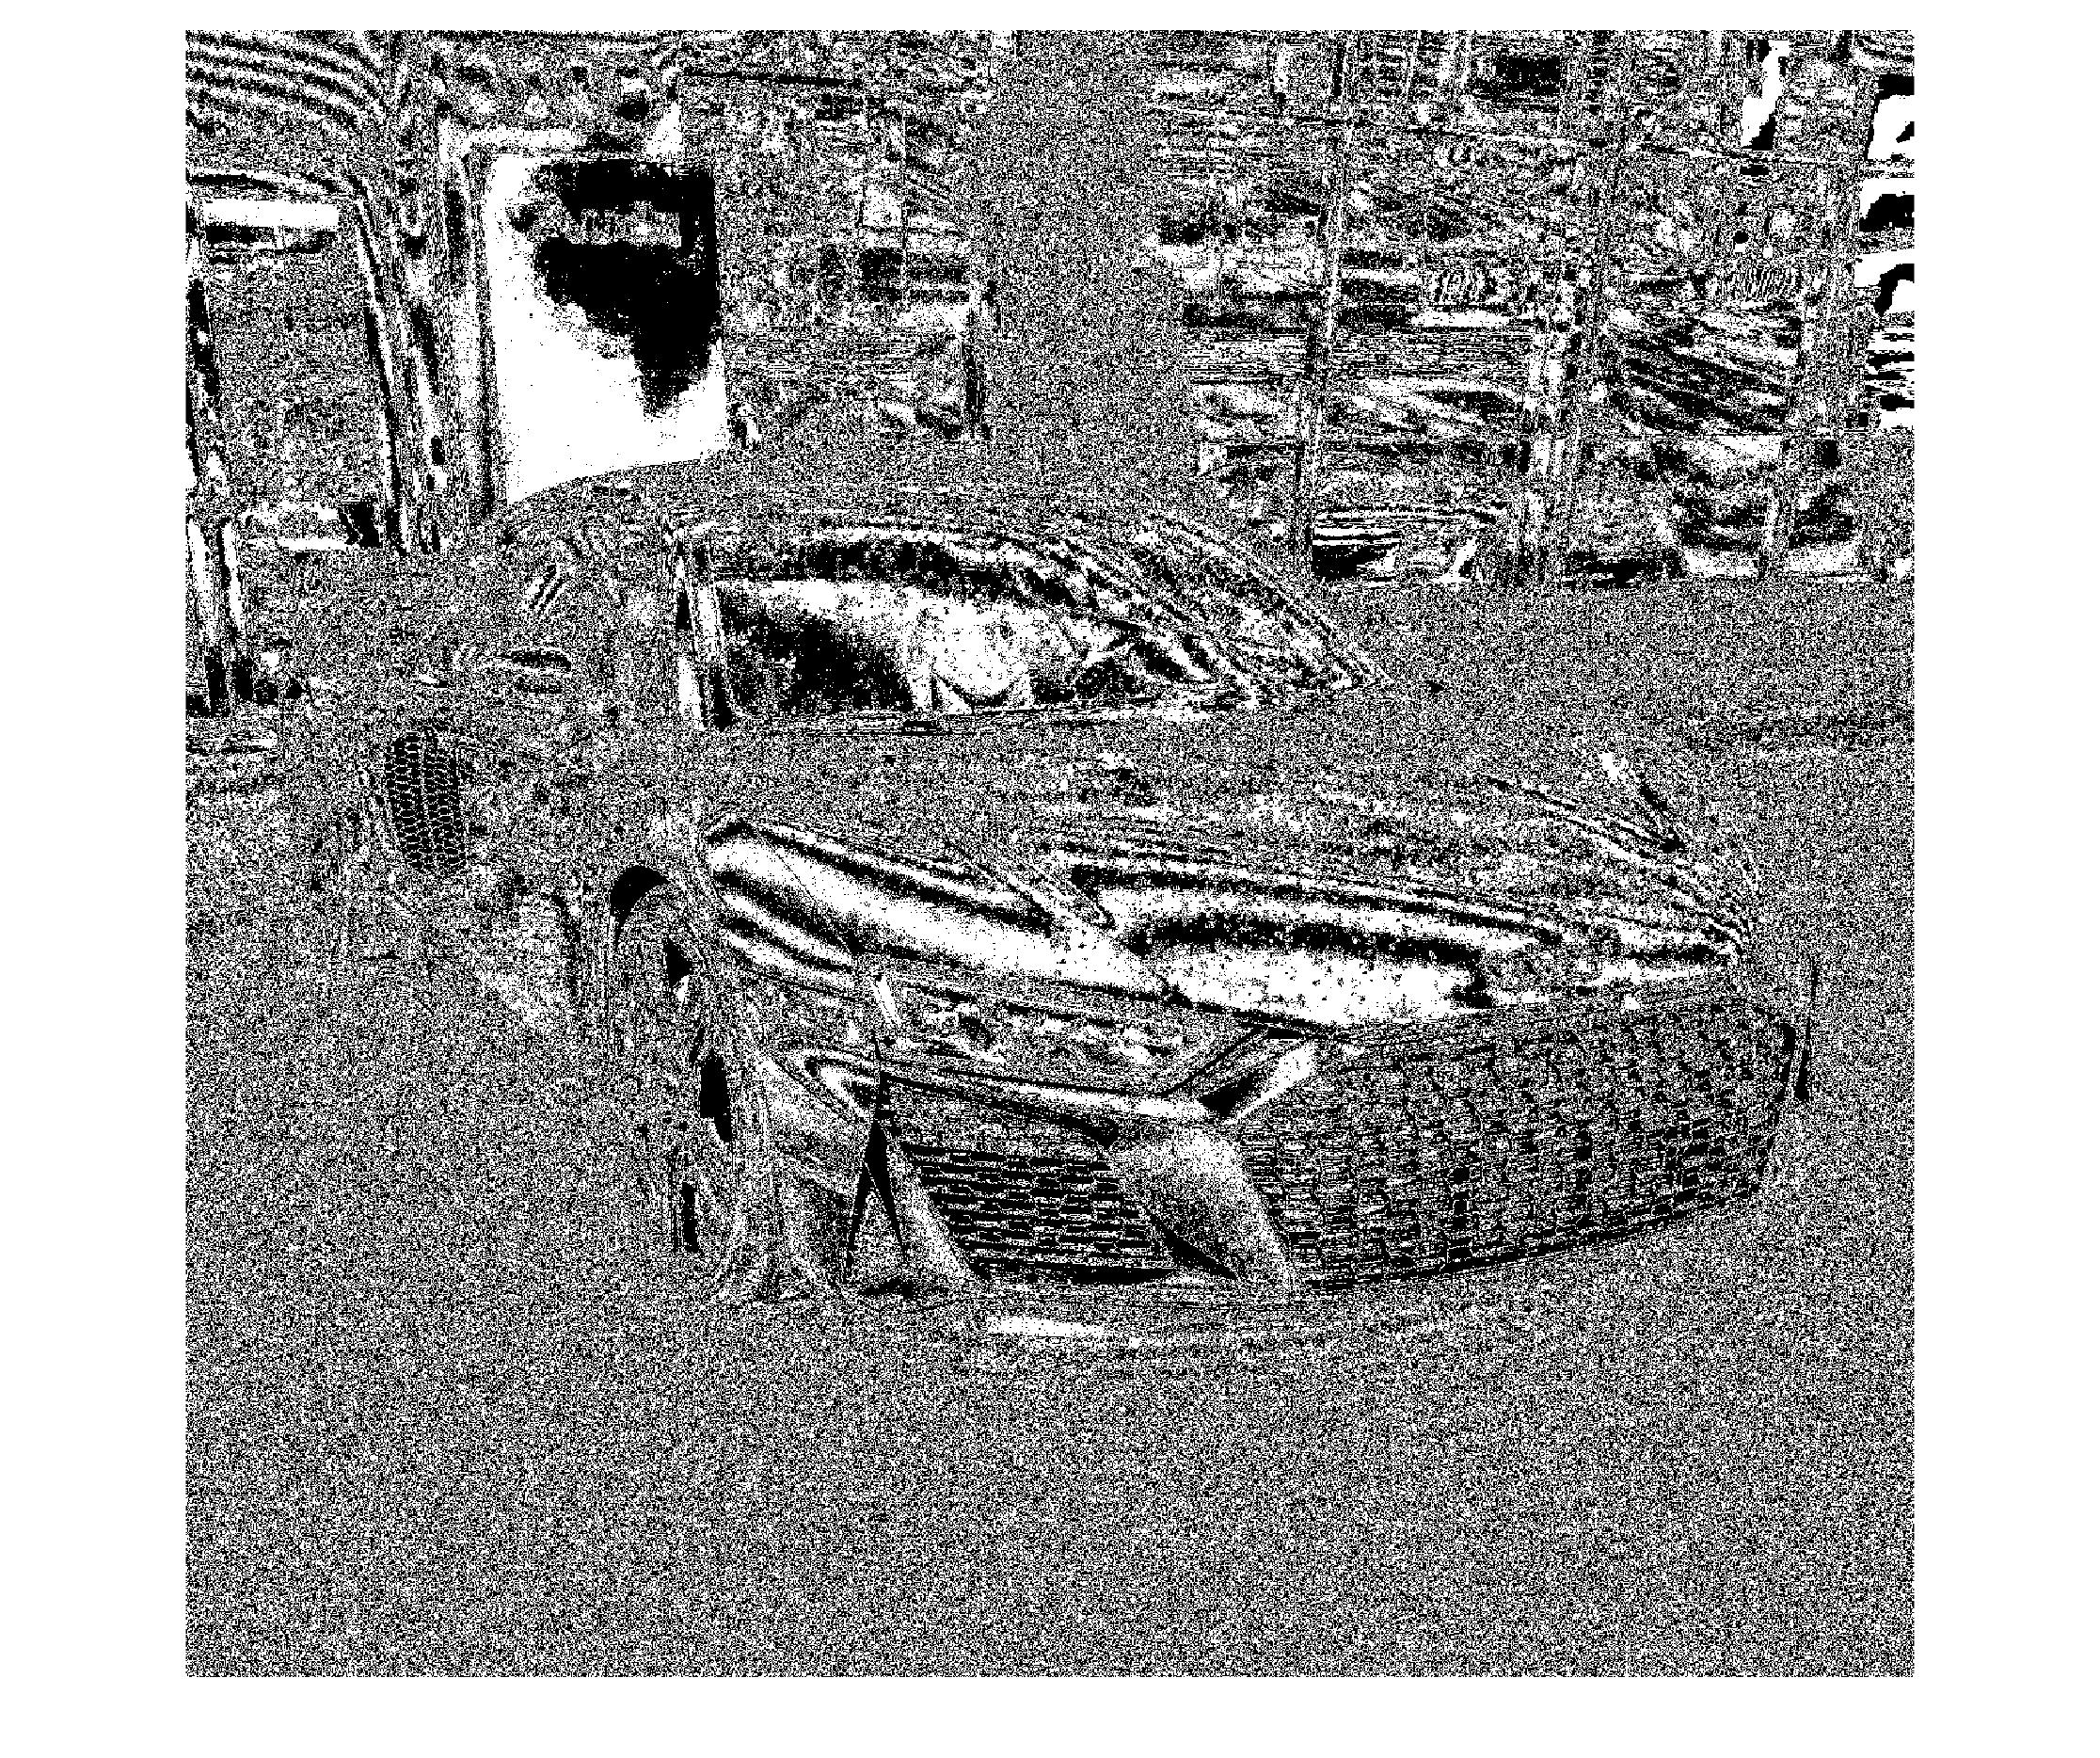
\includegraphics[width=\linewidth]{images/img7.jpg}
\caption{4\textsuperscript{th} bit-plane}
\end{subfigure}
\begin{subfigure}[b]{0.3\linewidth}
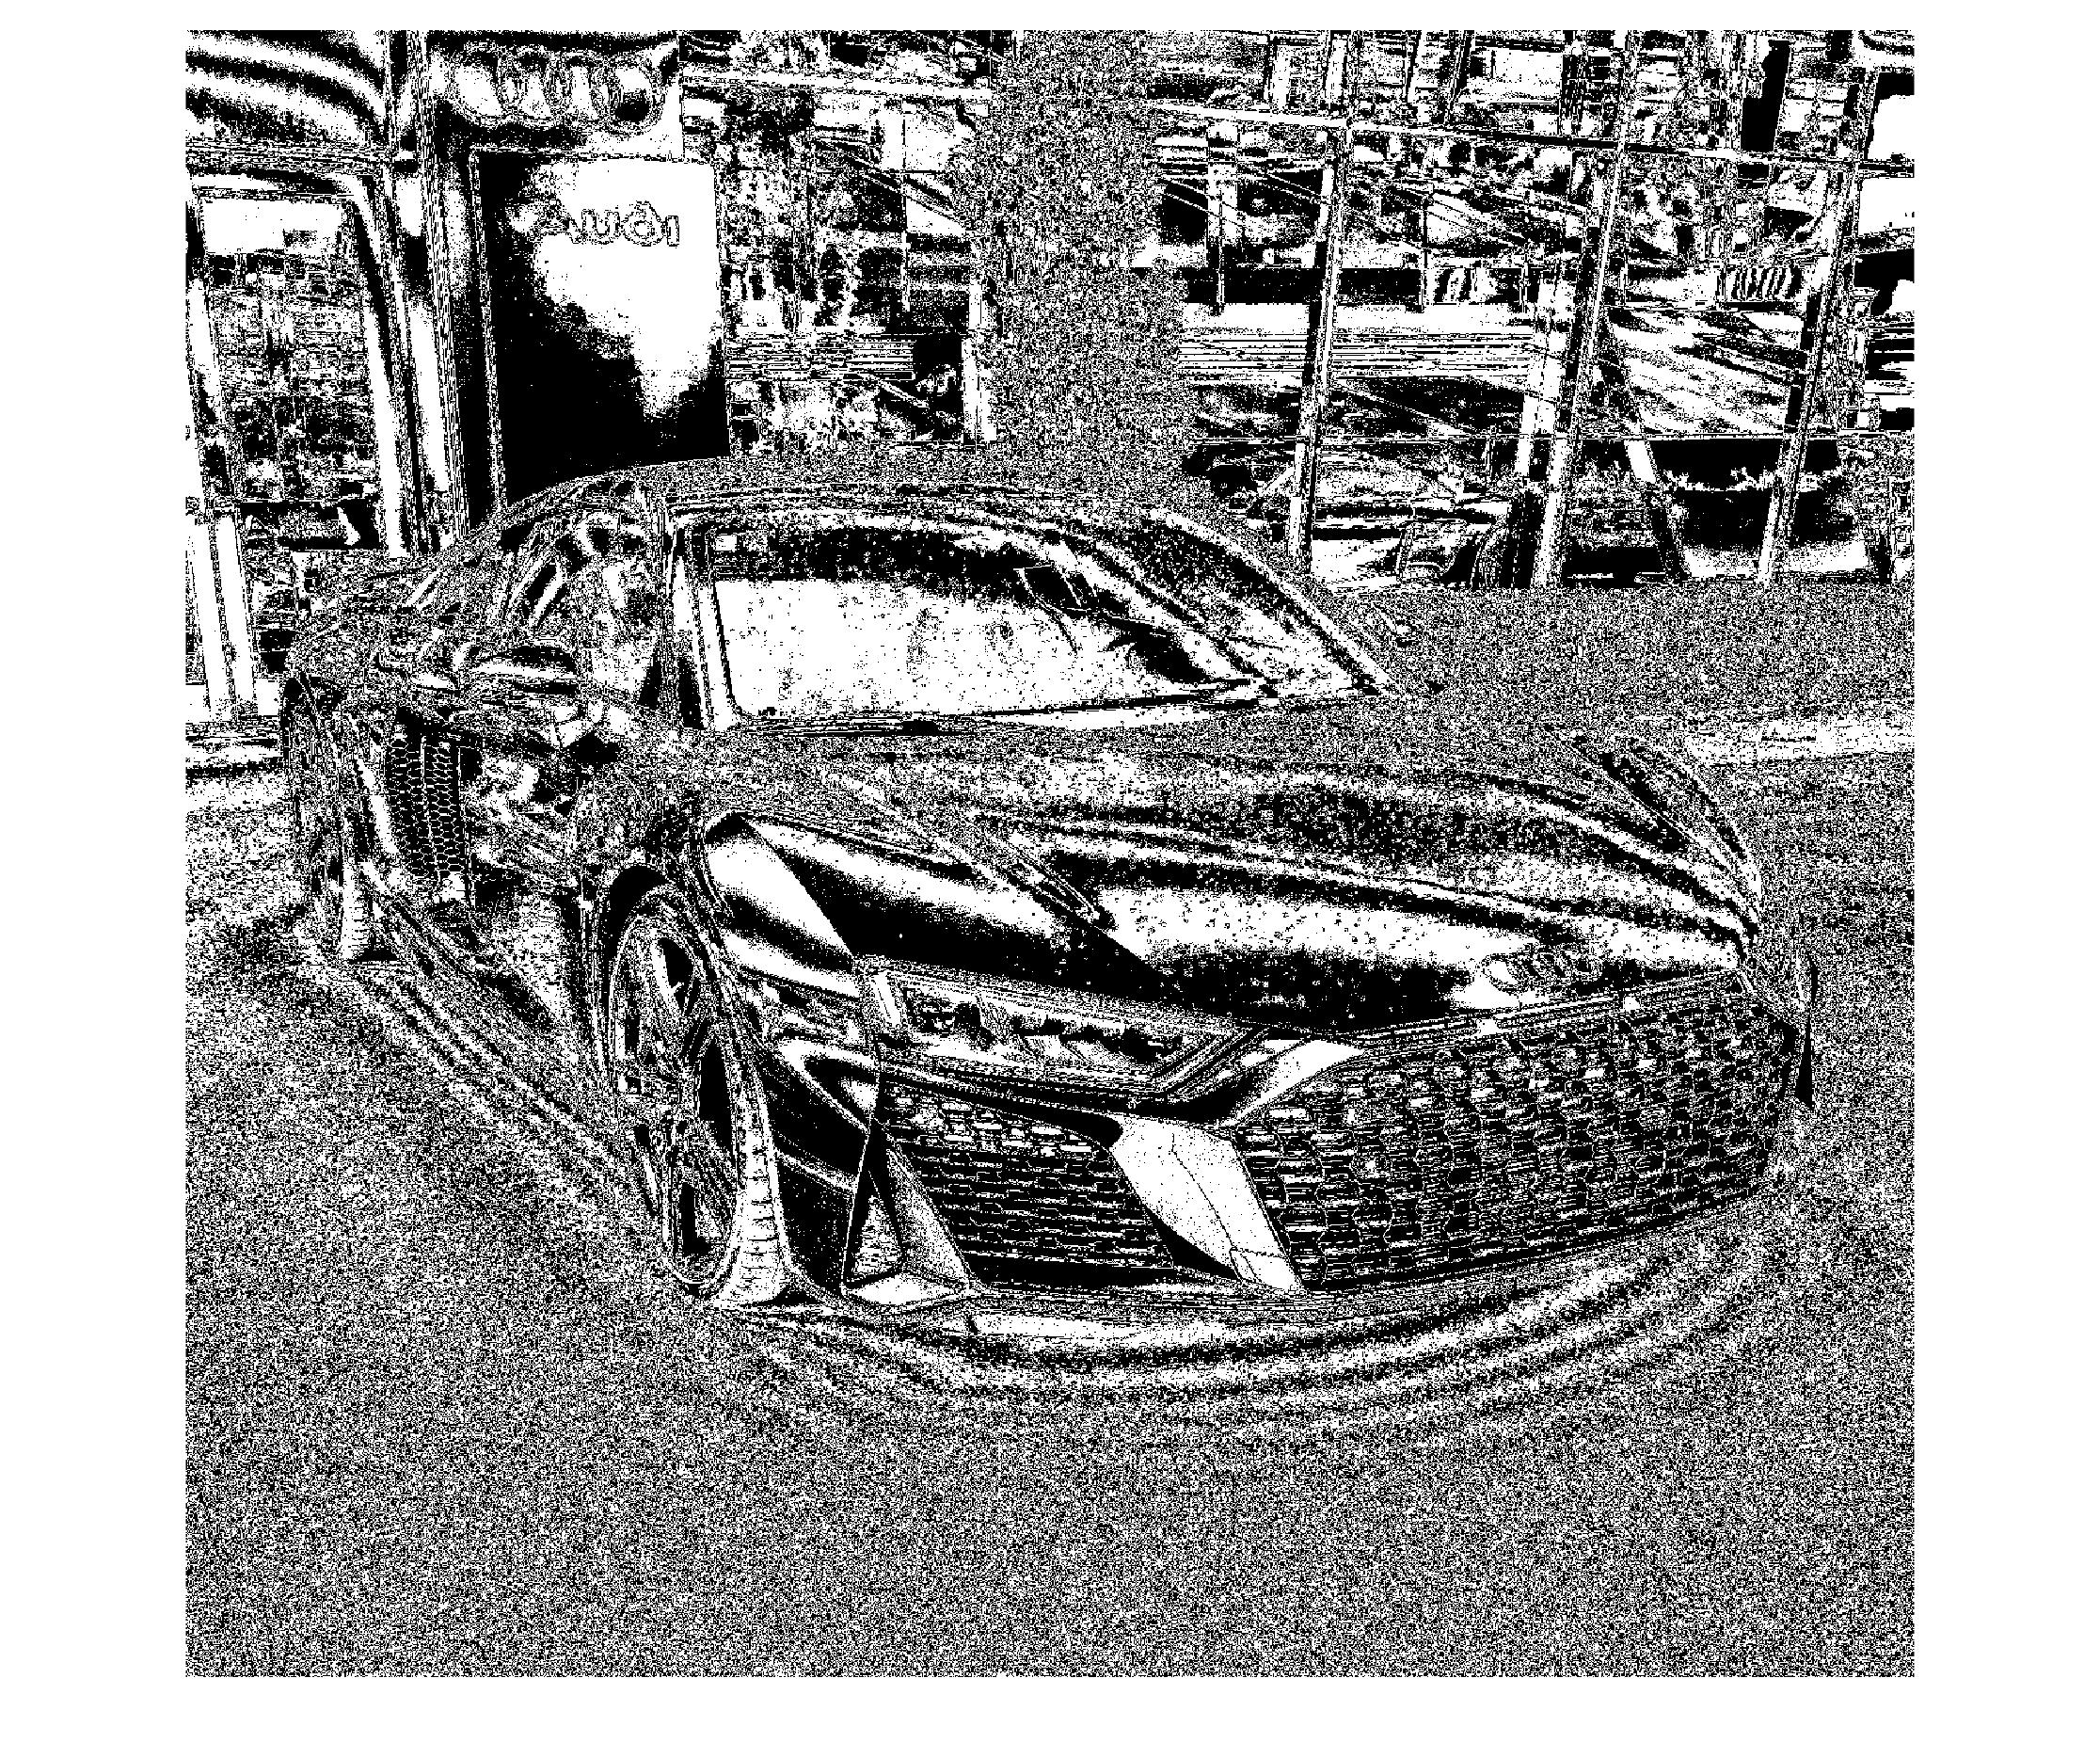
\includegraphics[width=\linewidth]{images/img8.jpg}
\caption{5\textsuperscript{th} bit-plane}
\end{subfigure}
\begin{subfigure}[b]{0.3\linewidth}
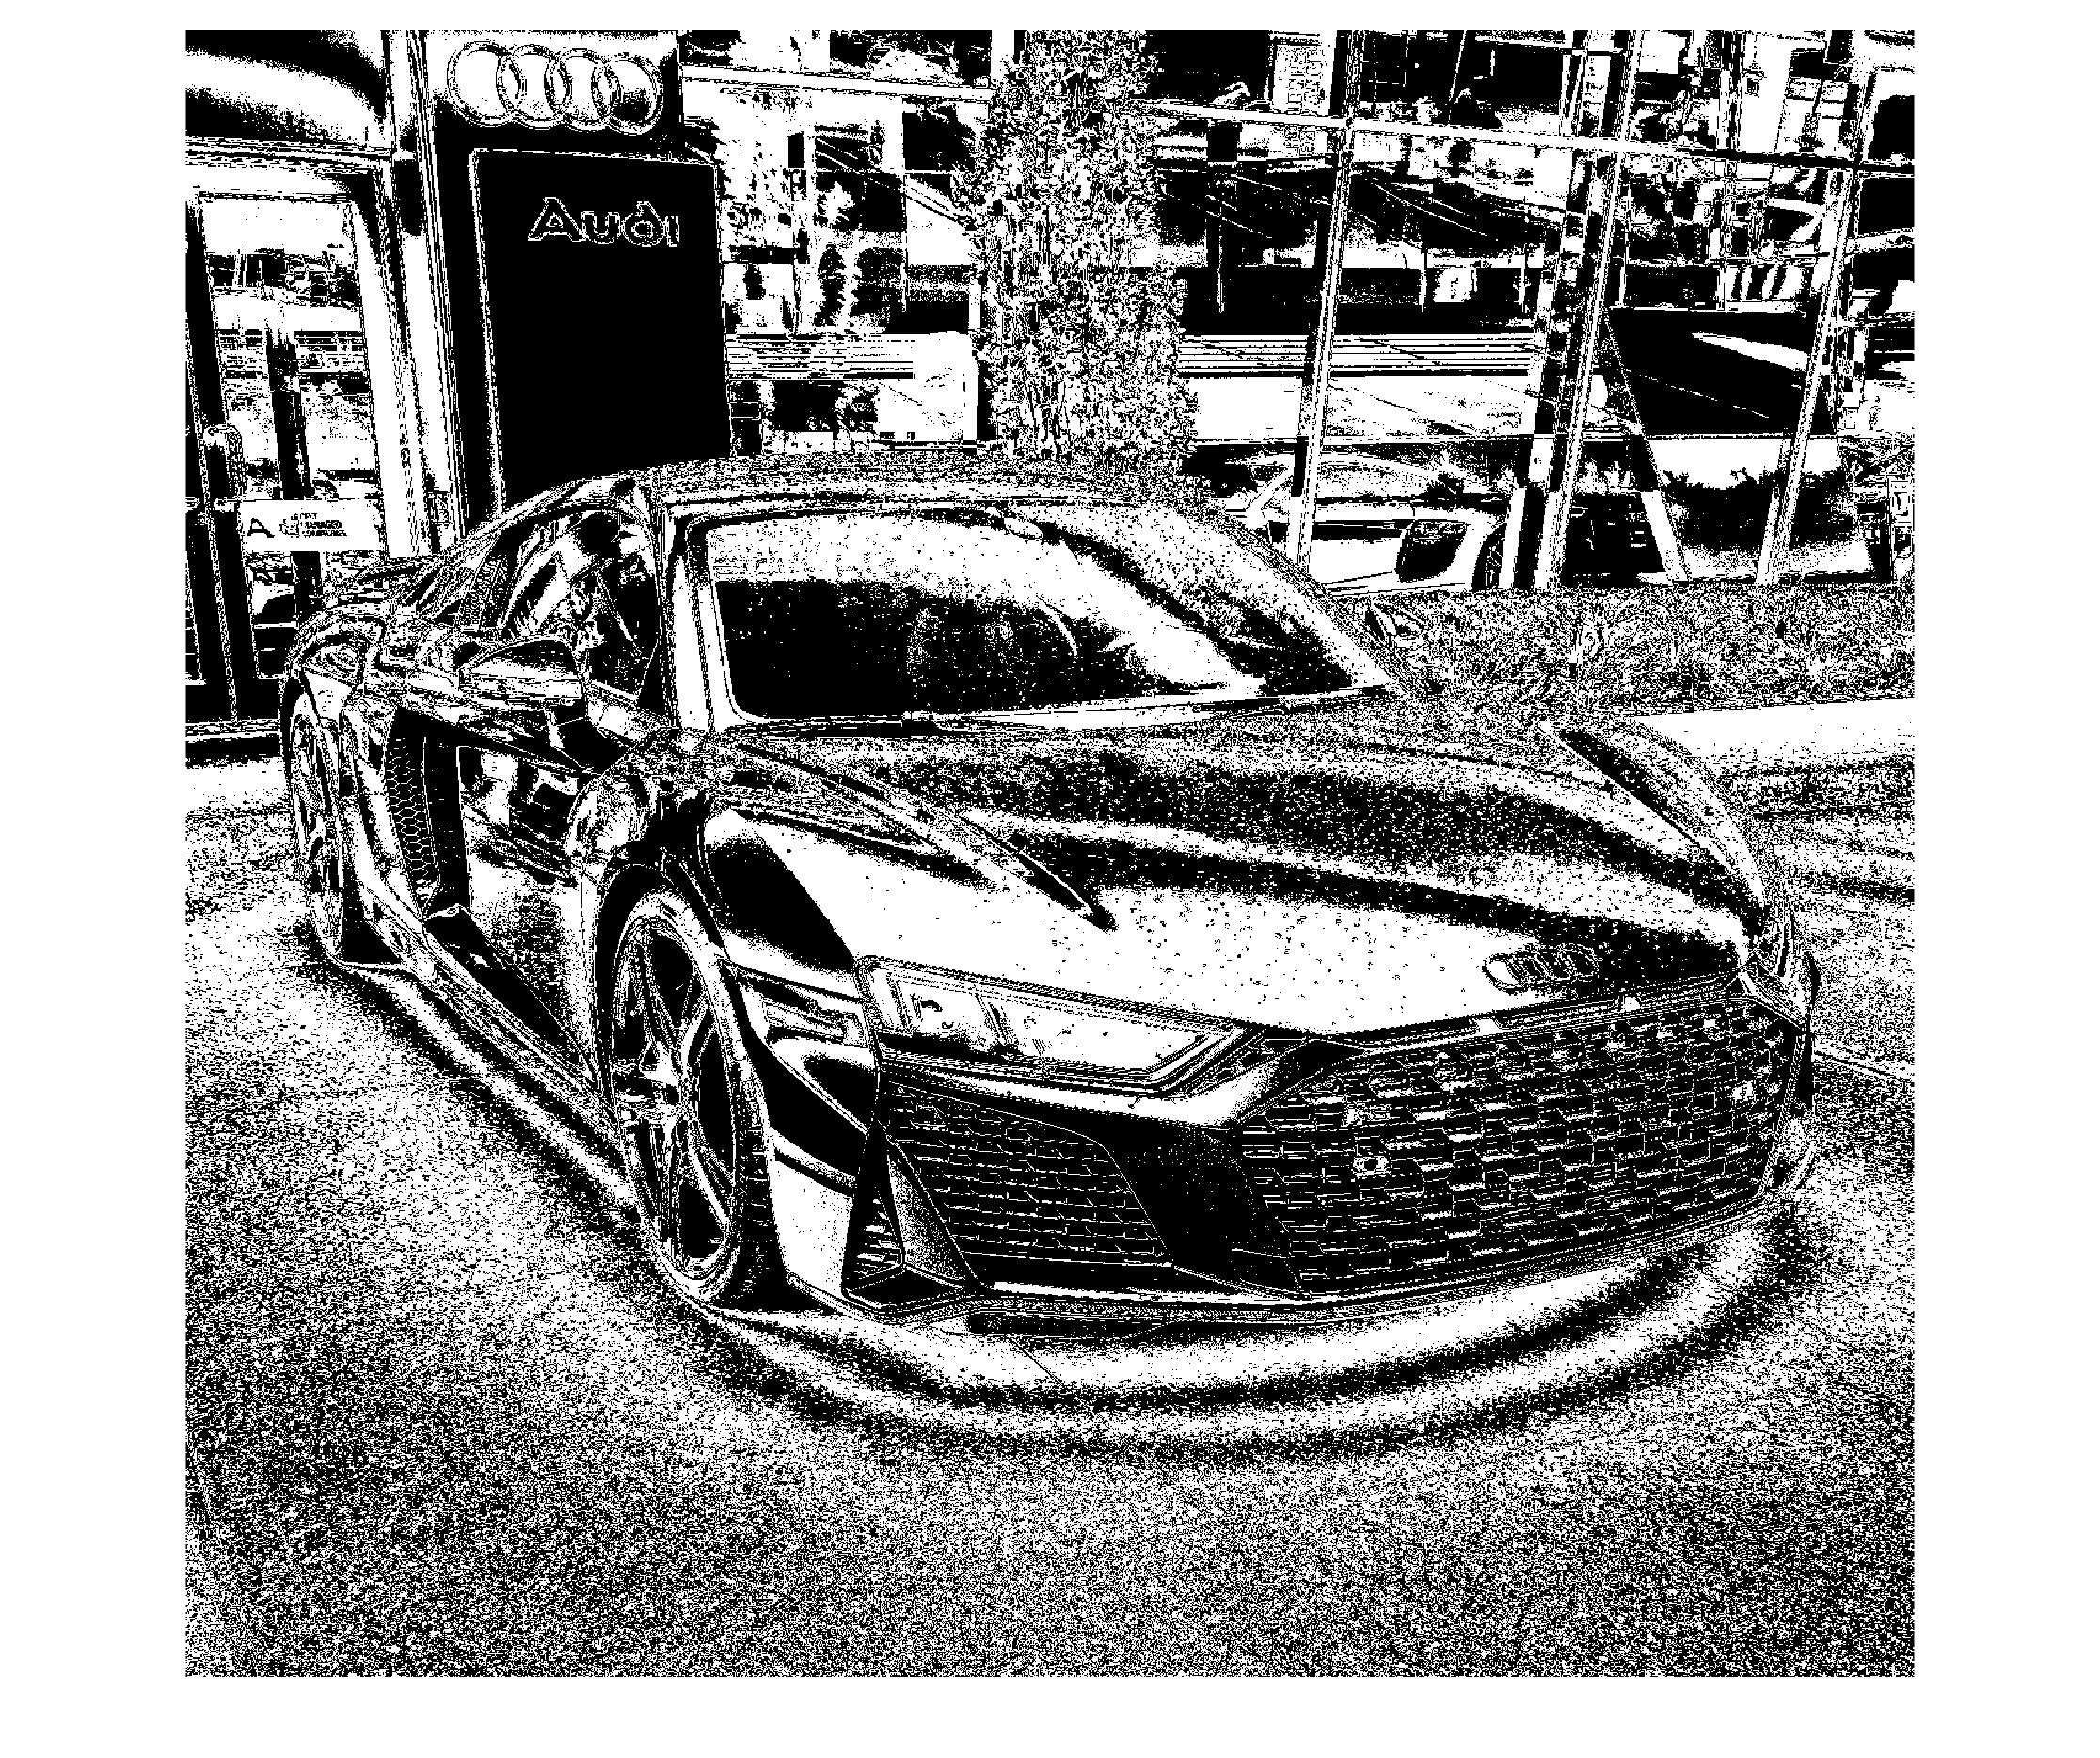
\includegraphics[width=\linewidth]{images/img9.jpg}
\caption{6\textsuperscript{th} bit-plane}
\end{subfigure}
\begin{subfigure}[b]{0.3\linewidth}
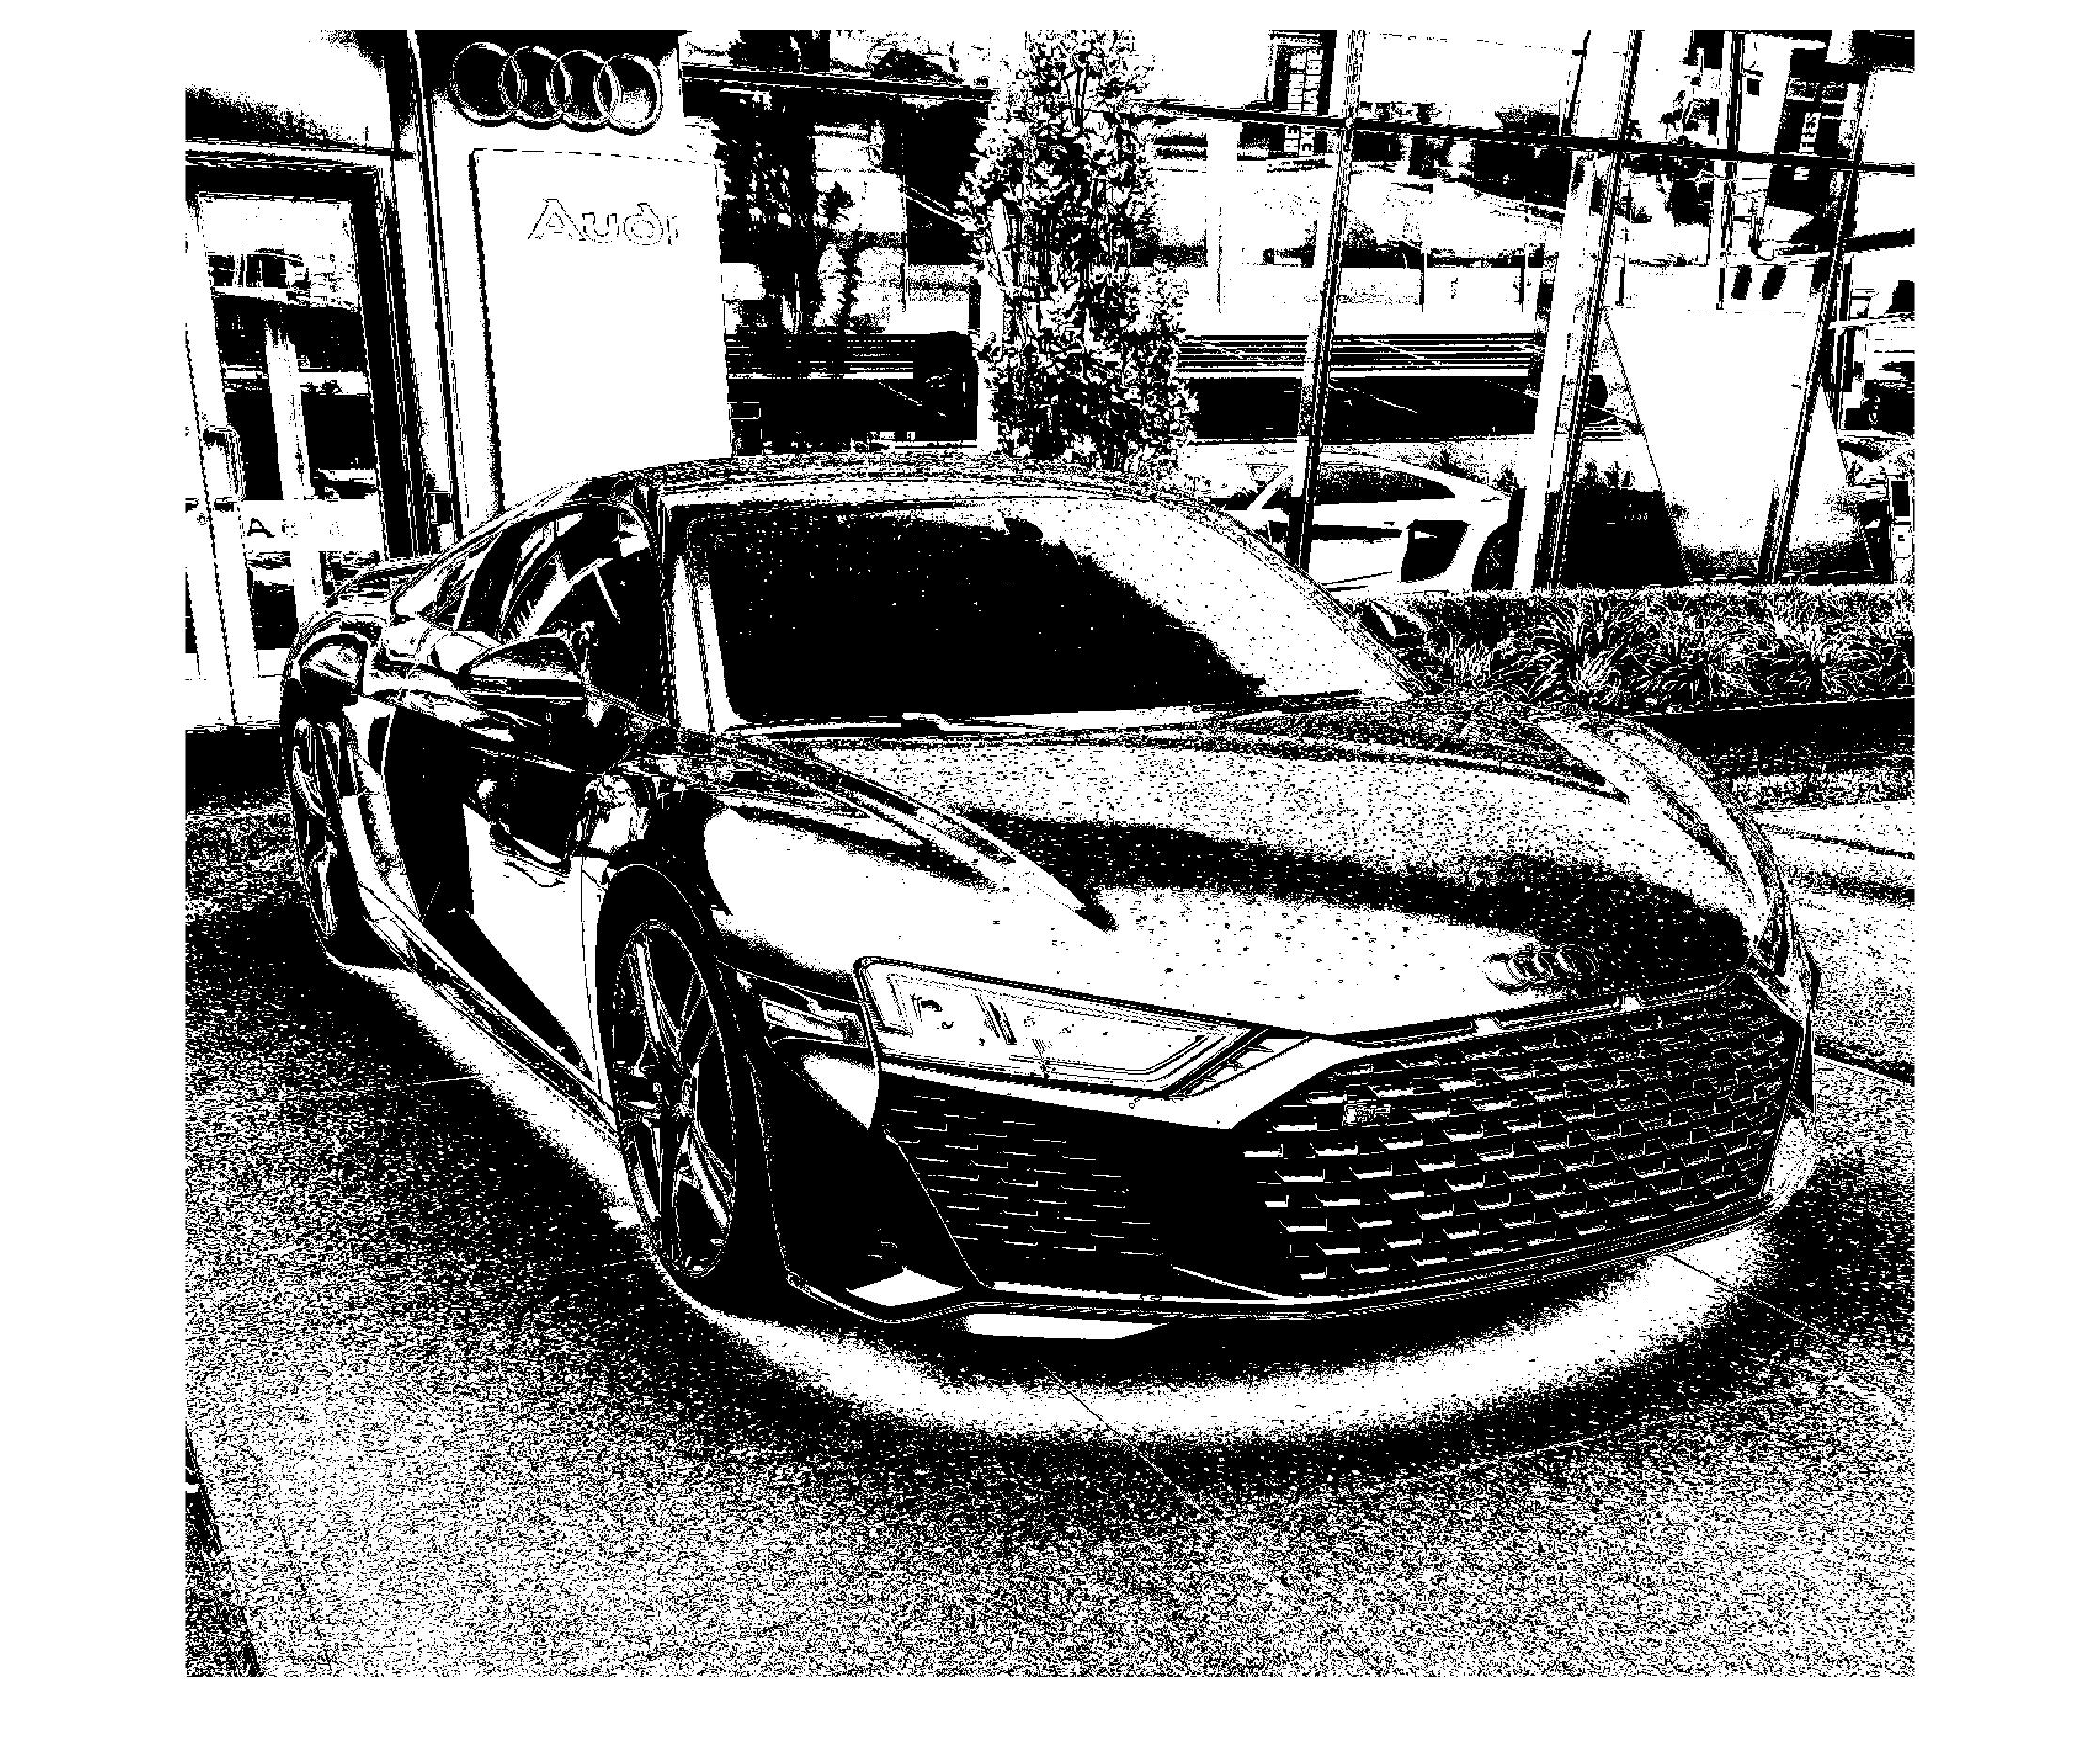
\includegraphics[width=\linewidth]{images/img10.jpg}
\caption{7\textsuperscript{th} bit-plane}
\end{subfigure}
\begin{subfigure}[b]{0.3\linewidth}
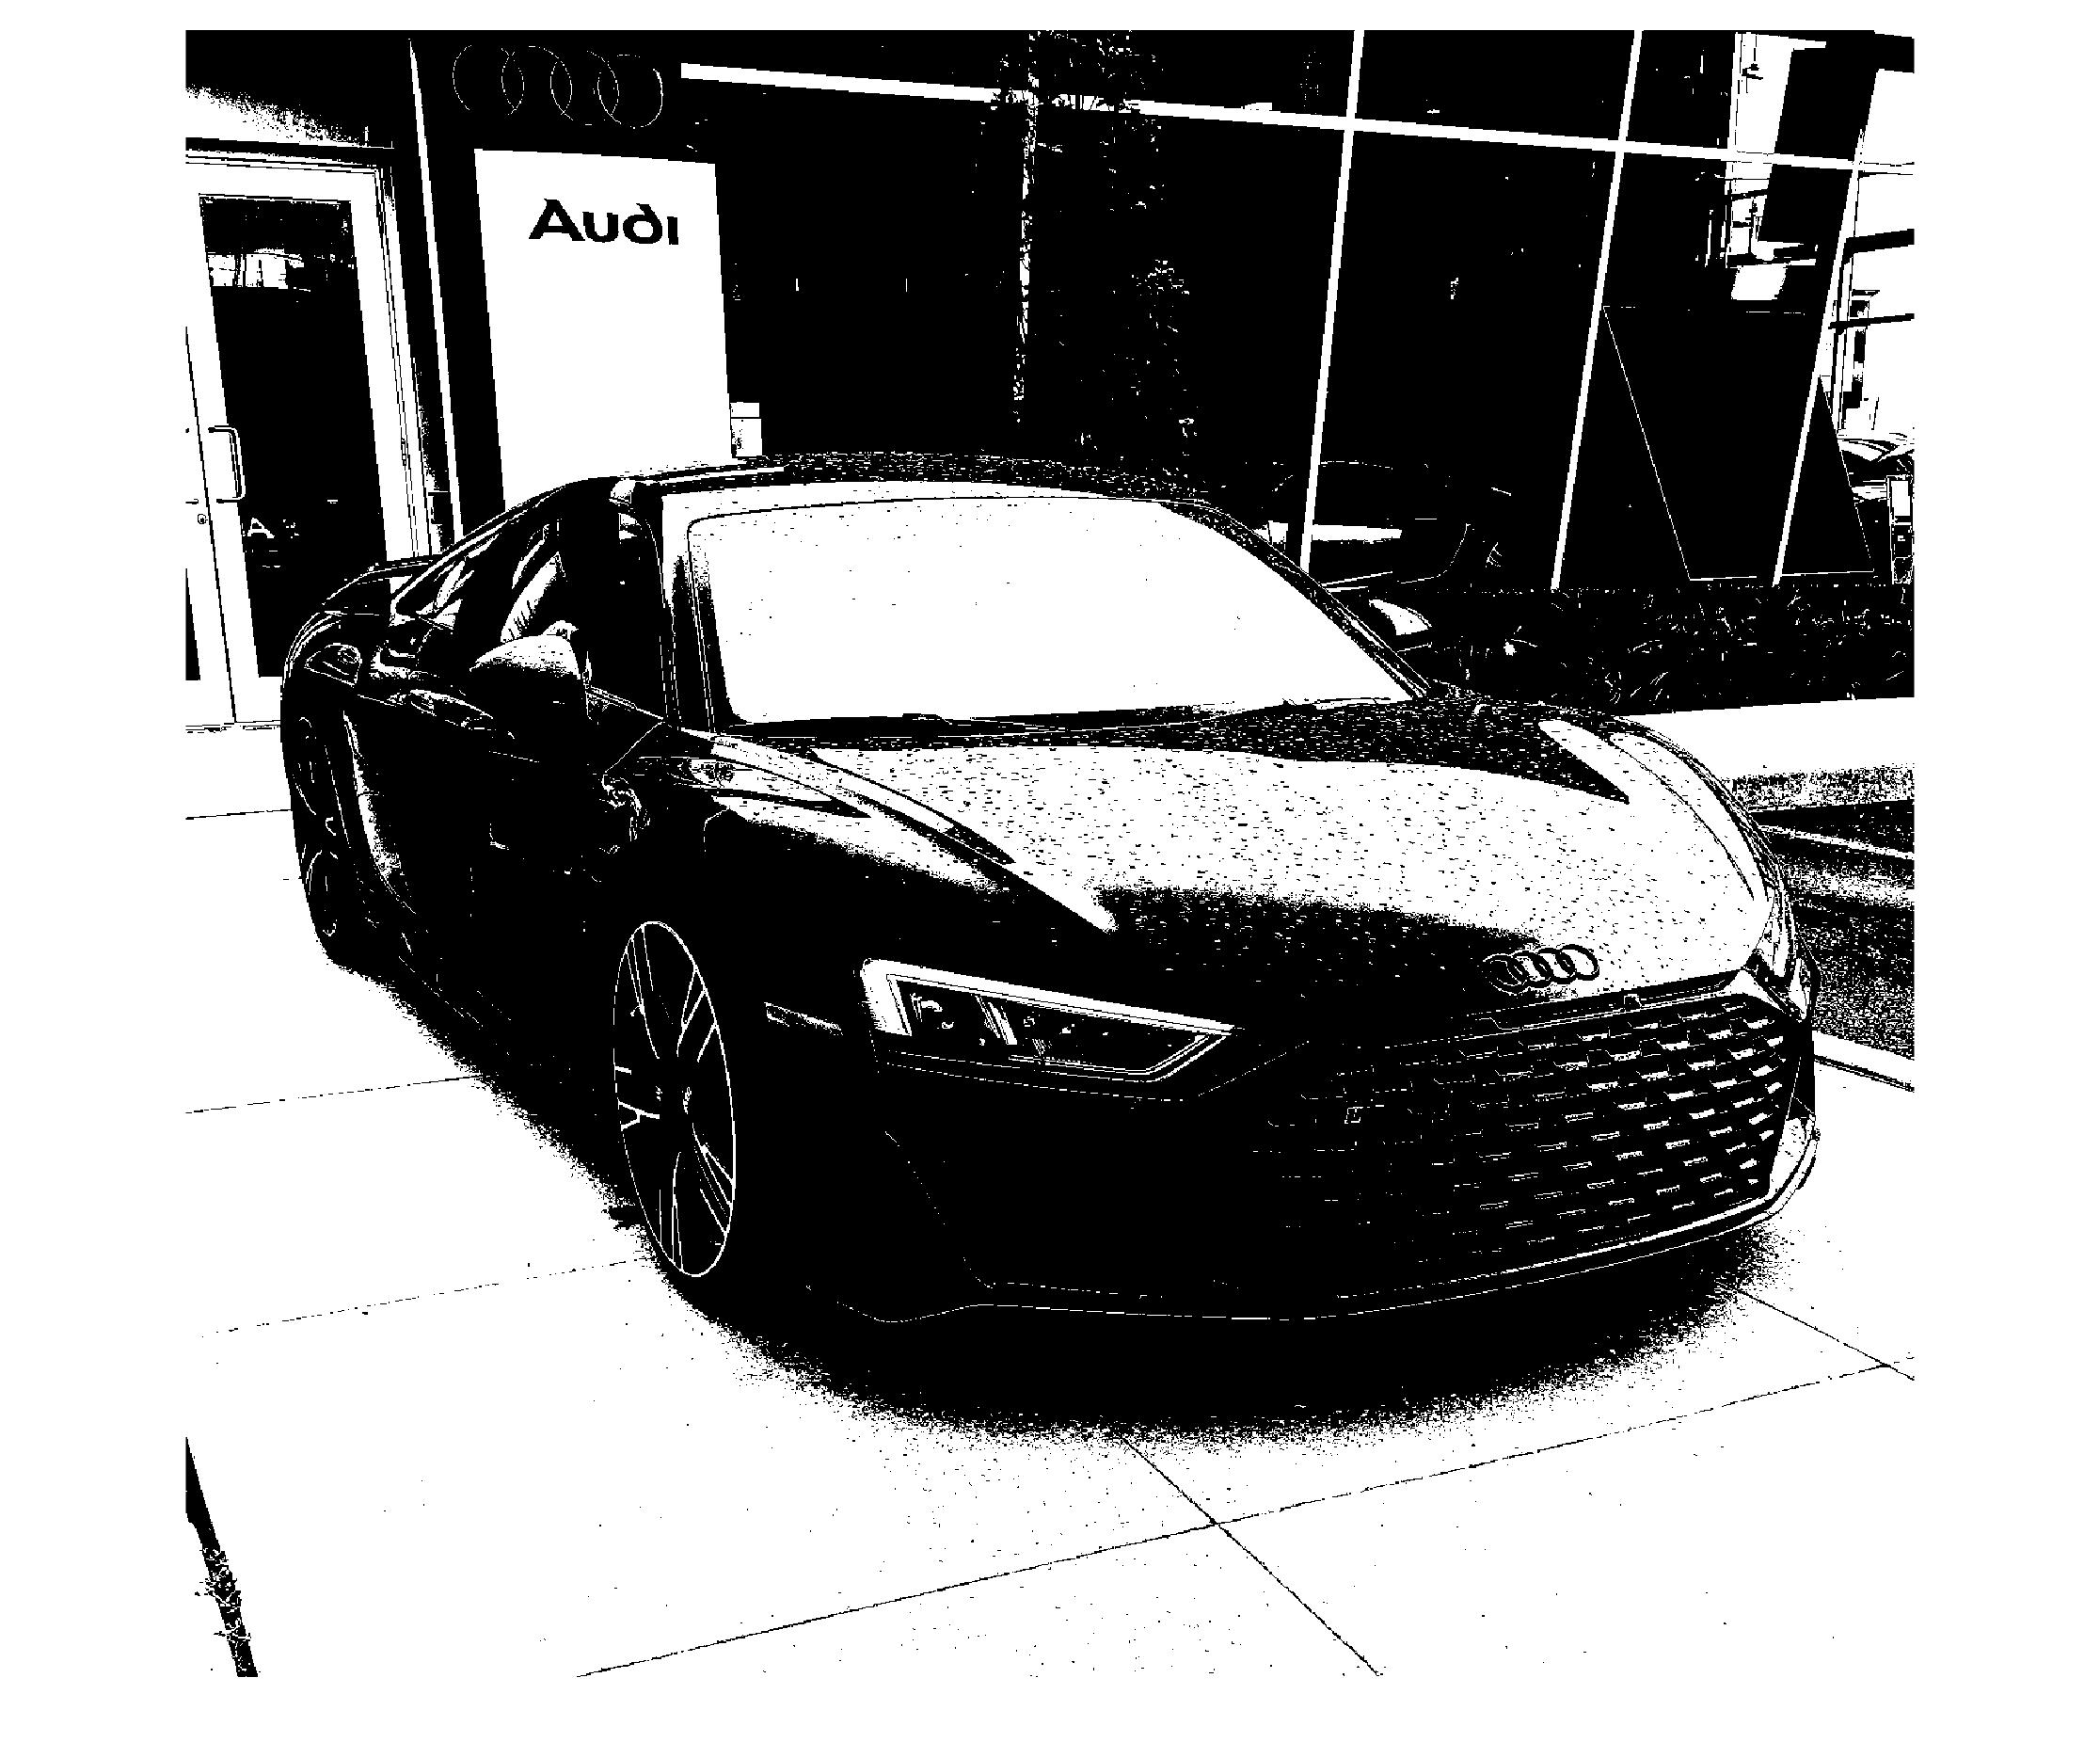
\includegraphics[width=\linewidth]{images/img11.jpg}
\caption{8\textsuperscript{th} bit-plane}
\end{subfigure}
\caption{Bit-plane slicing results}
\label{fig:bit-plane slicing results}
\end{figure}

\begin{lstlisting}[language=Matlab]
% Reconstruct the image from 
% the highest 2 bit-planes 
reconstructed_img1=((2^7)*b8)+((2^6)*b7);

% Reconstruct the image from 
% the highest 4 bit-planes
reconstructed_img2=((2^7)*b8)+((2^6)*b7) 
                +((2^5)*b6)+((2^4)*b5);

figure;
imshow(gray_img)
figure;
imshow(reconstructed_img1)
figure;
imshow(reconstructed_img2)

\end{lstlisting}

\begin{figure}[h!]
\centering
\begin{subfigure}[b]{0.3\linewidth}
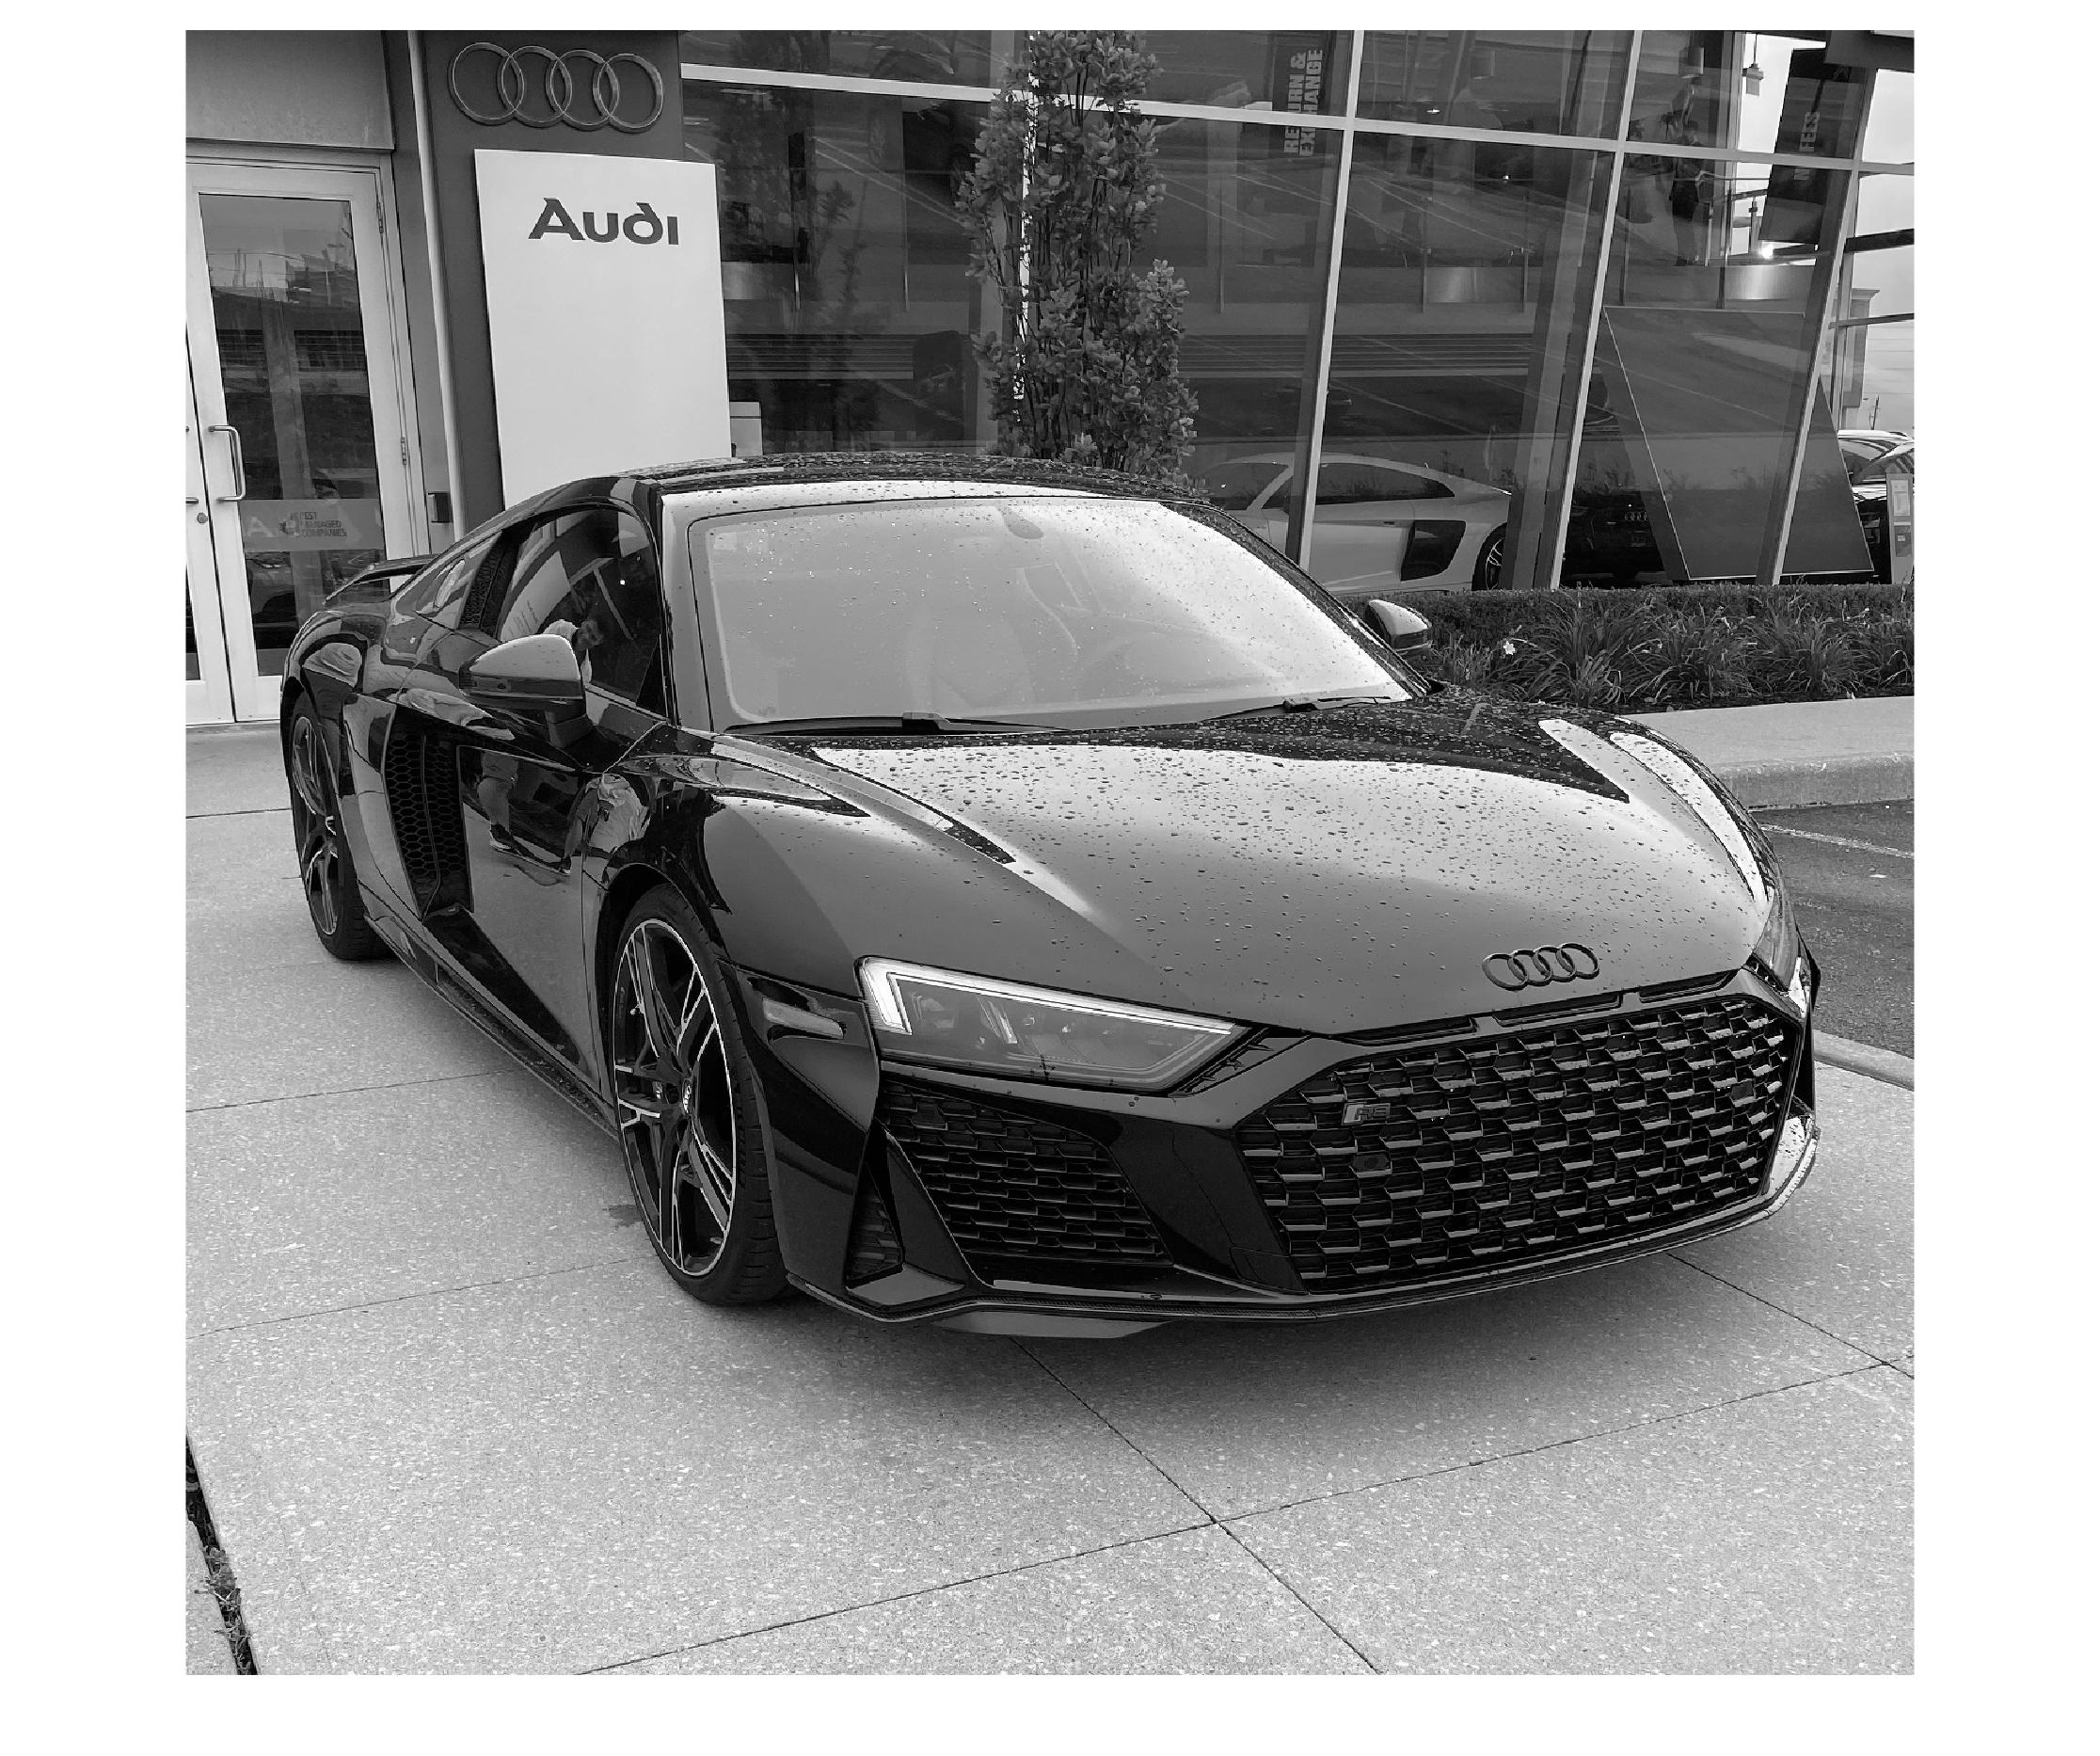
\includegraphics[width=\linewidth]{images/img1.jpg}
\caption{Grayscale}
\end{subfigure}
\begin{subfigure}[b]{0.3\linewidth}
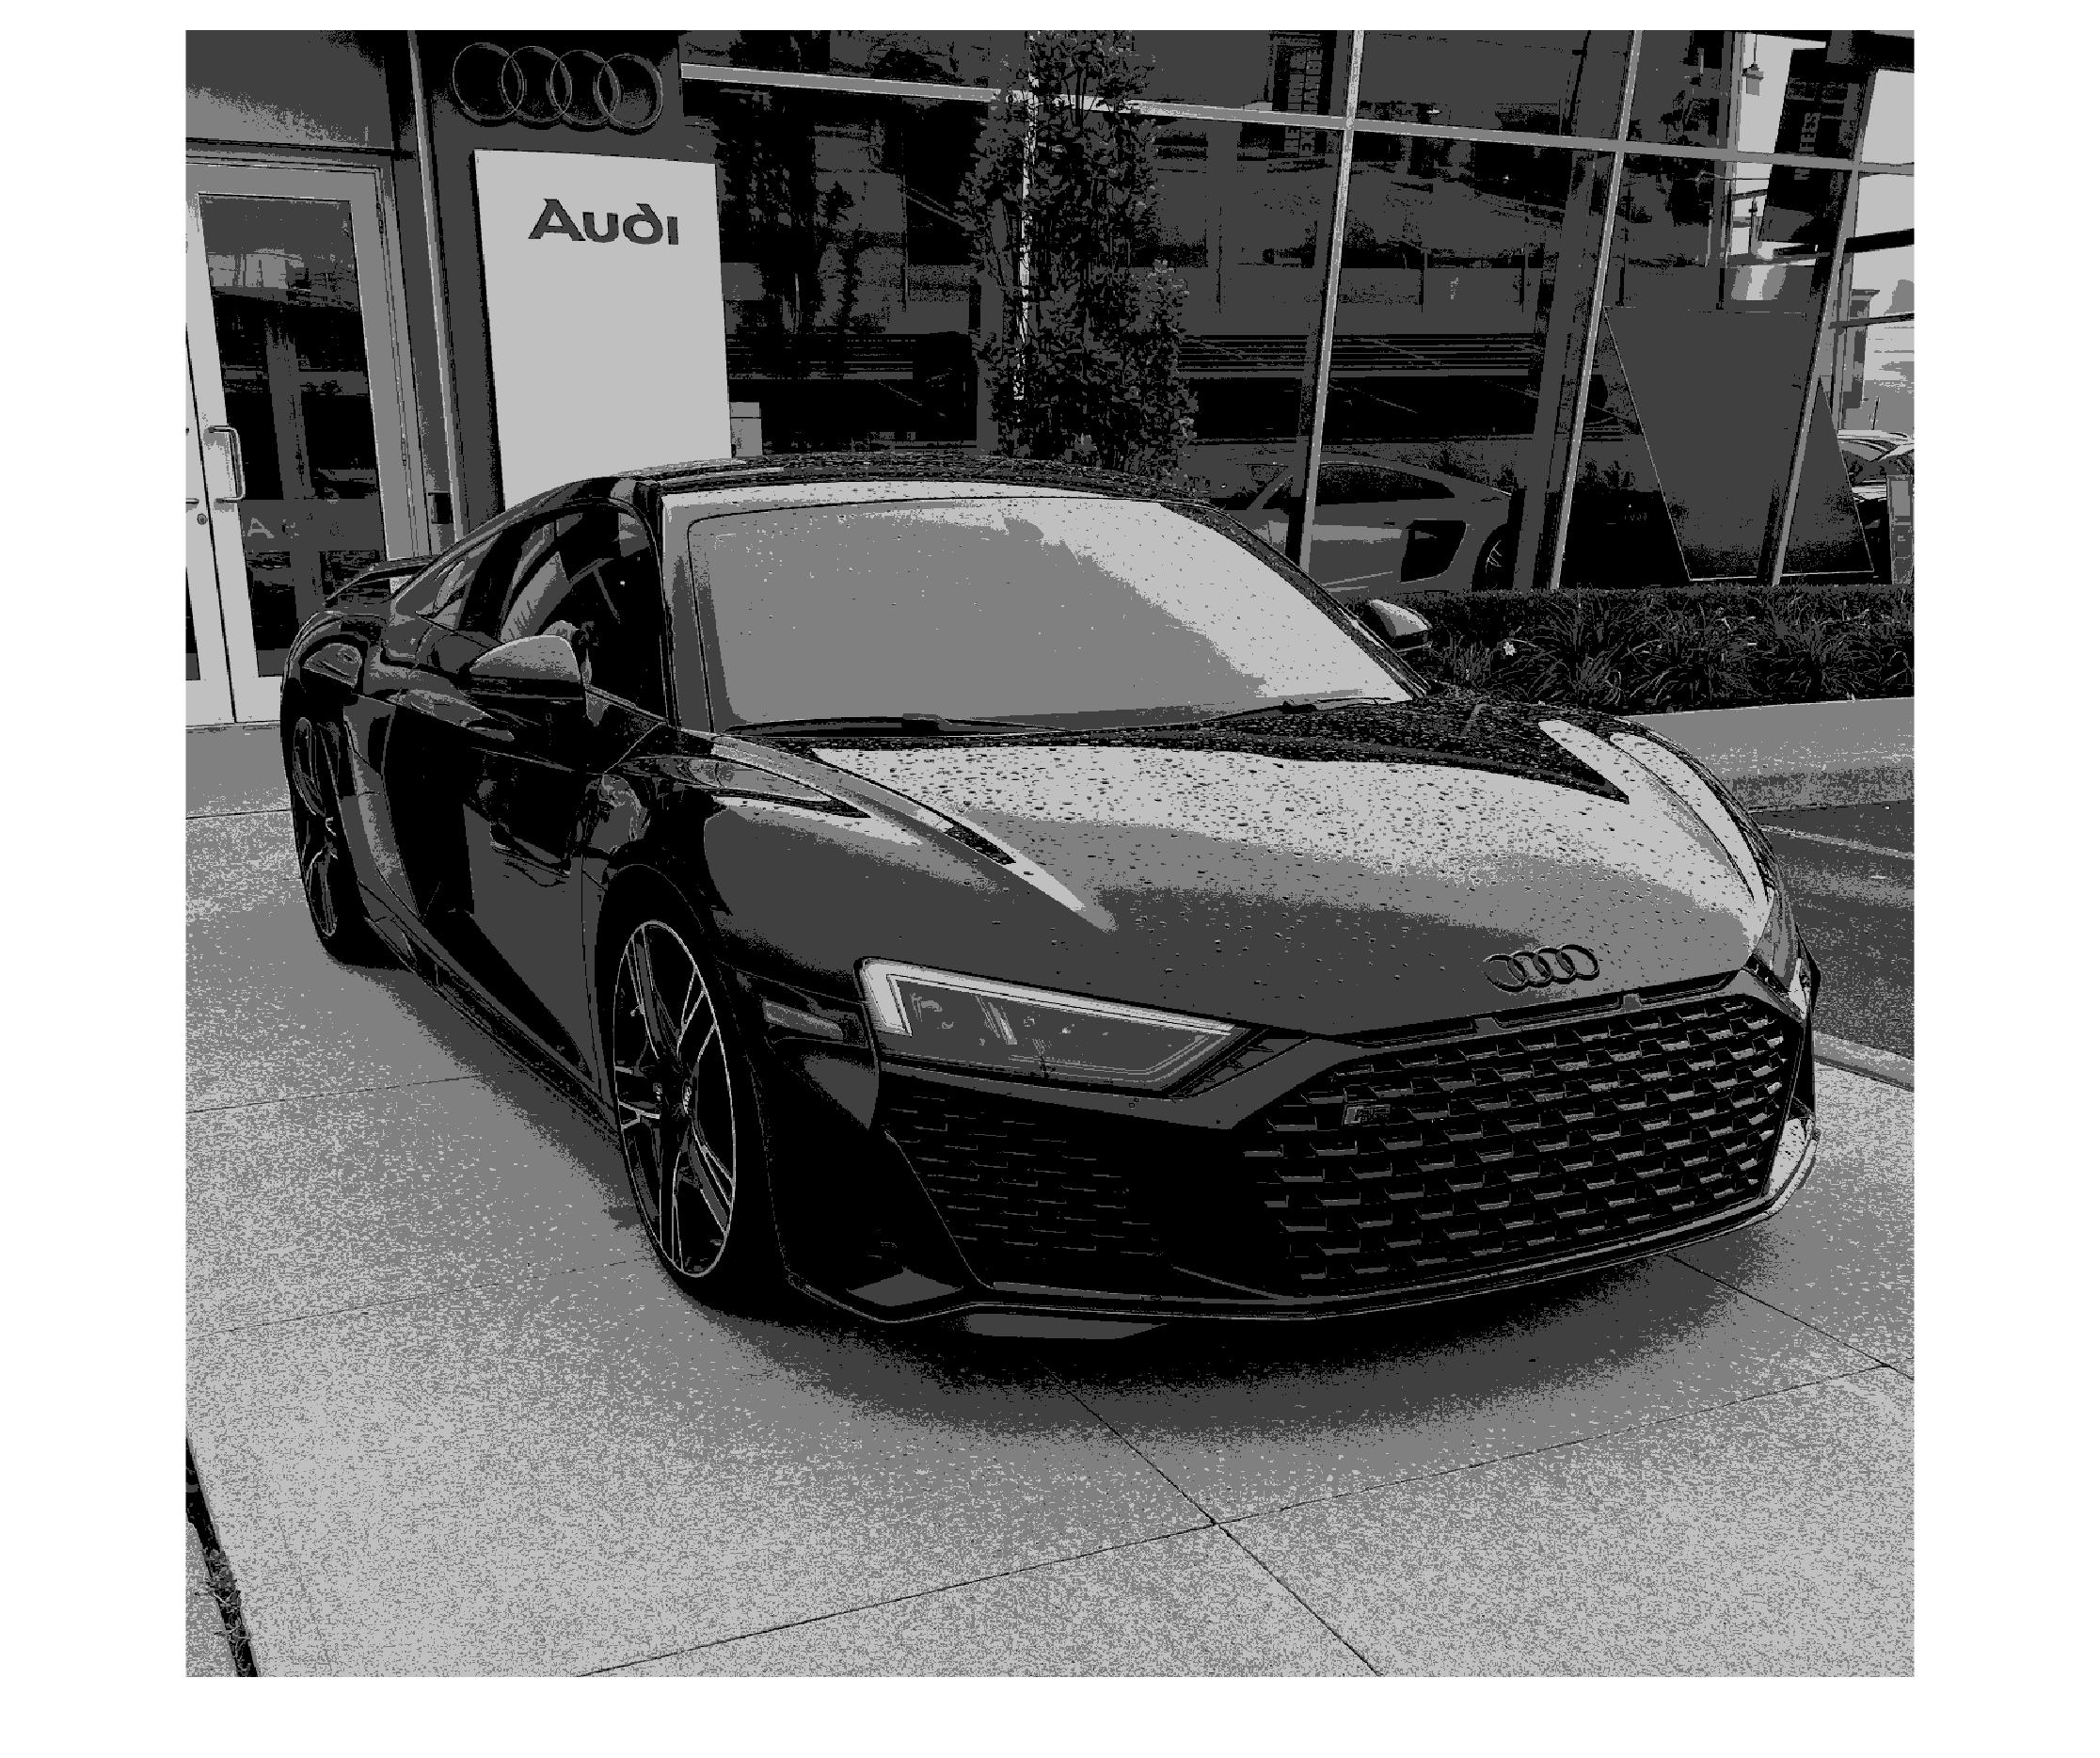
\includegraphics[width=\linewidth]{images/img12.jpg}
\caption{bit planes 8 and 7}
\end{subfigure}
\begin{subfigure}[b]{0.3\linewidth}
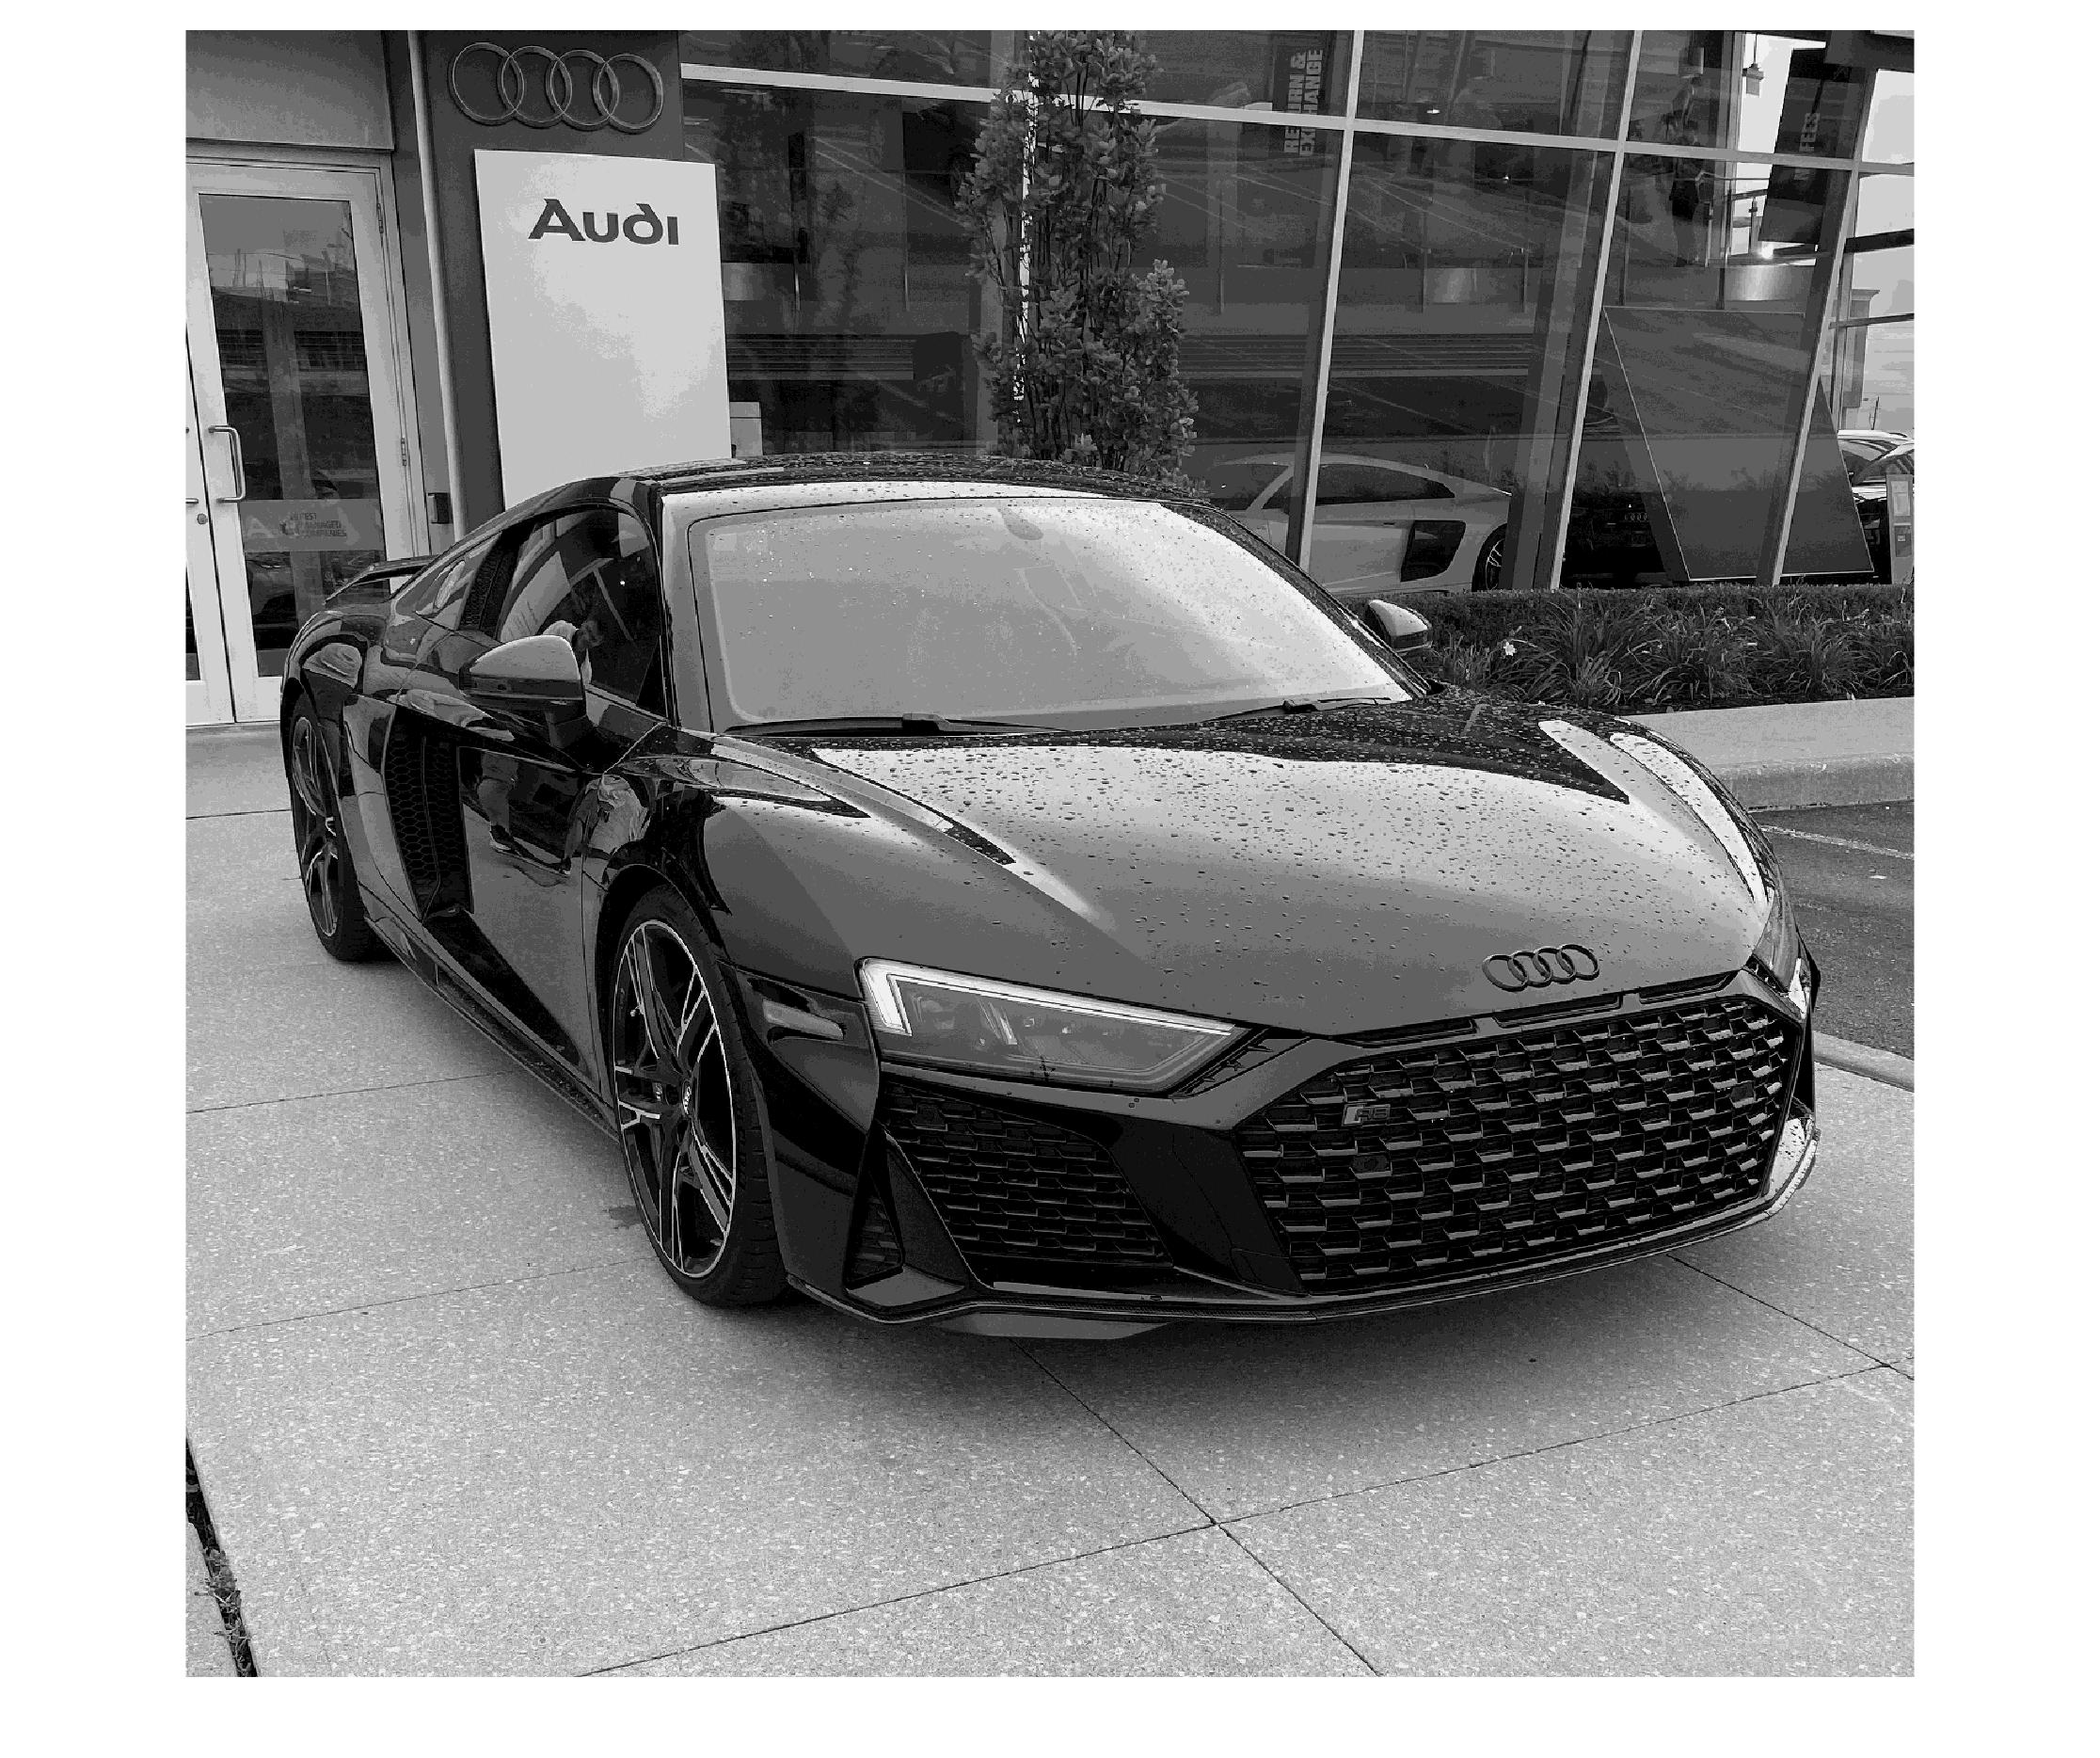
\includegraphics[width=\linewidth]{images/img13.jpg}
\caption{bit planes 8, 7, 6 and 5}
\end{subfigure}
\caption{Reconstructed images from bit-plane slicing}
\label{fig:Reconstructed images from bit-plane slicing}
\end{figure}

Separating a digital image into its bit planes is useful for analyzing the relative importance played by each bit of the image, implying, it determines the adequacy of numbers of bits used to quantize each pixel , useful for image compression.

\newpage
\subsection{Problem 3}

\begin{lstlisting}[language=Matlab]
% Load the original image
img=imread('/lamnguyen/Desktop/School
/Computer-Vision/A1/images/AudiR8.jpg');

% Convert the image to grayscale
gray_img = rgb2gray(img);

% Perform power-law transformation 
% on the grayscale image
% Gamma equals to 0.3 
img1 = imadjust(gray_img, [], [], 0.3);

% Gamma equals to 3
img2 = imadjust(gray_img, [], [], 3);

% Equalize the histogram of images
hist_gray = histeq(gray_img, 256);
hist1 = histeq(img1, 256);
hist2 = histeq(img2, 256);

% Display histograms and images 
% before and after equalization
figure;
imshow(gray_img)
figure;
imshow(hist_gray)
figure;
imhist(gray_img)
figure;
imhist(hist_gray, 256)
figure;
imshow(img1)
figure;
imshow(hist1)
figure;
imhist(img1)
figure;
imhist(hist1, 256)
figure;
imshow(img2)
figure;
imshow(hist2)
figure;
imhist(img2)
figure;
imhist(hist2, 256)
\end{lstlisting}

Histogram equalization is a computer image processing technique used to improve contrast in images. It accomplishes this by effectively spreading out the most frequent intensity values. This method usually increases the global contrast of images when its usable data is represented by close contrast values. This allows for areas of lower local contrast to gain a higher contrast.

\begin{figure}[h!]
\centering
\begin{subfigure}[b]{0.4\linewidth}
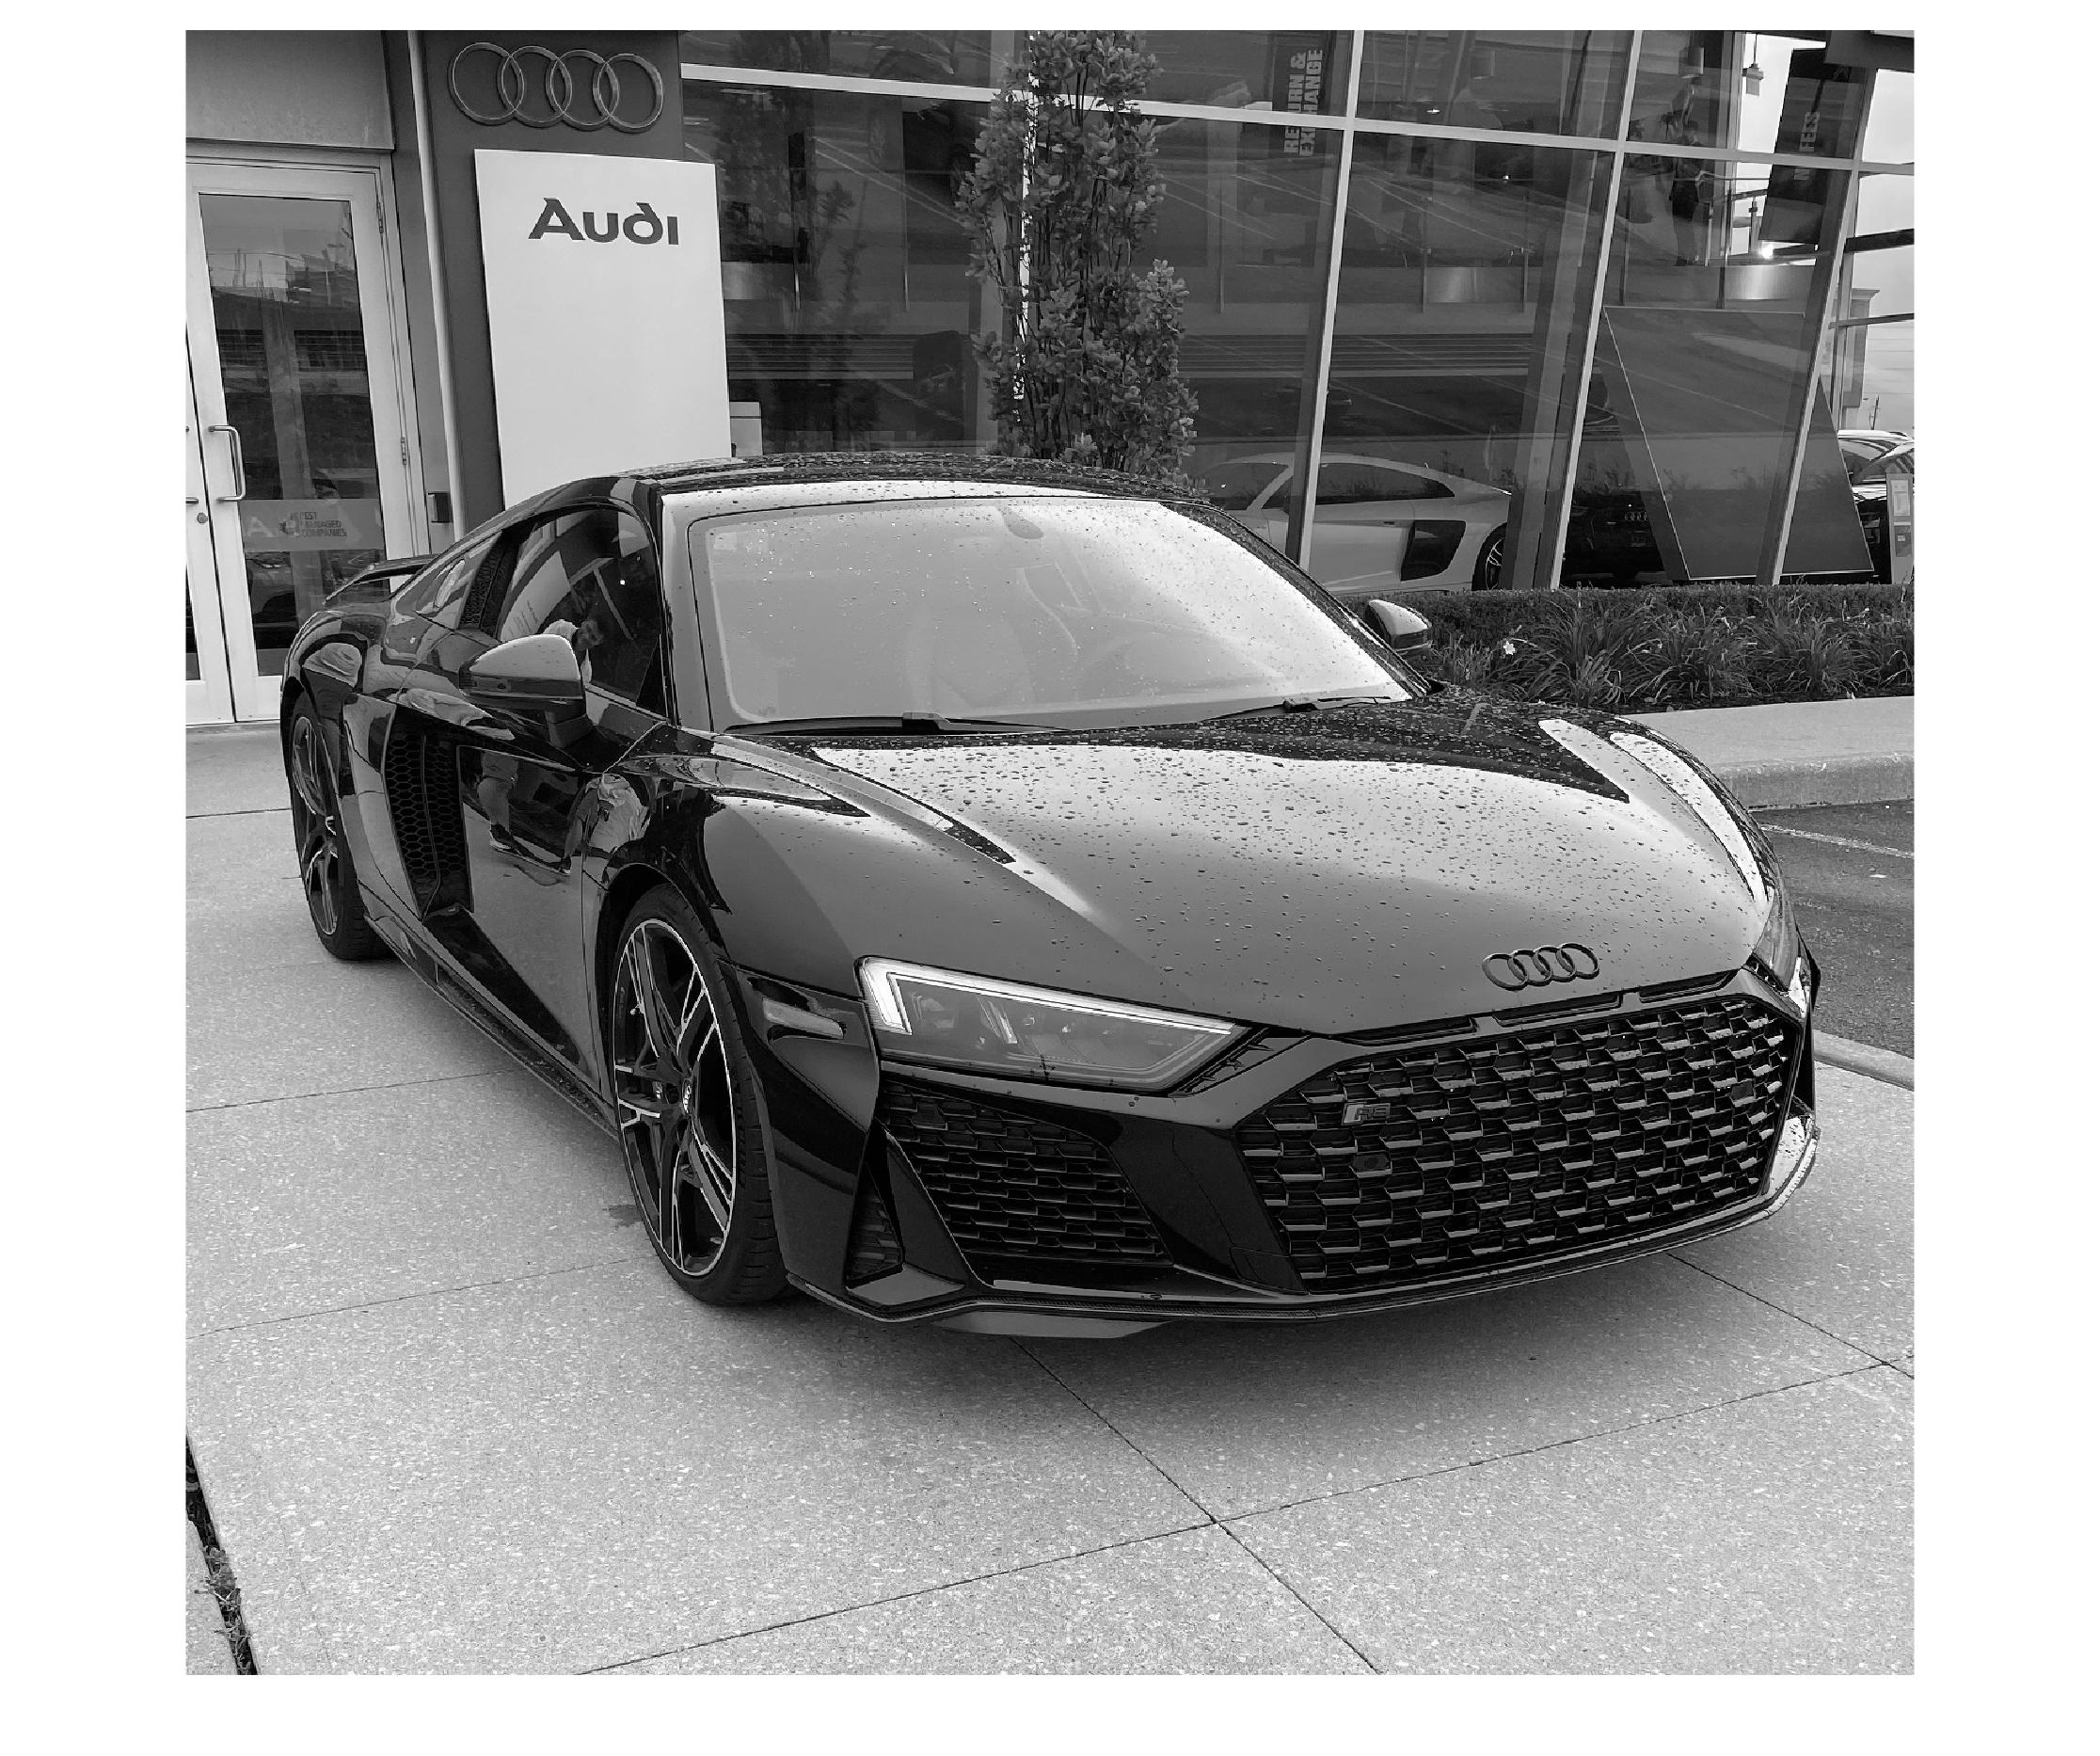
\includegraphics[width=\linewidth]{images/img1.jpg}
\caption{Before equalization}
\end{subfigure}
\begin{subfigure}[b]{0.4\linewidth}
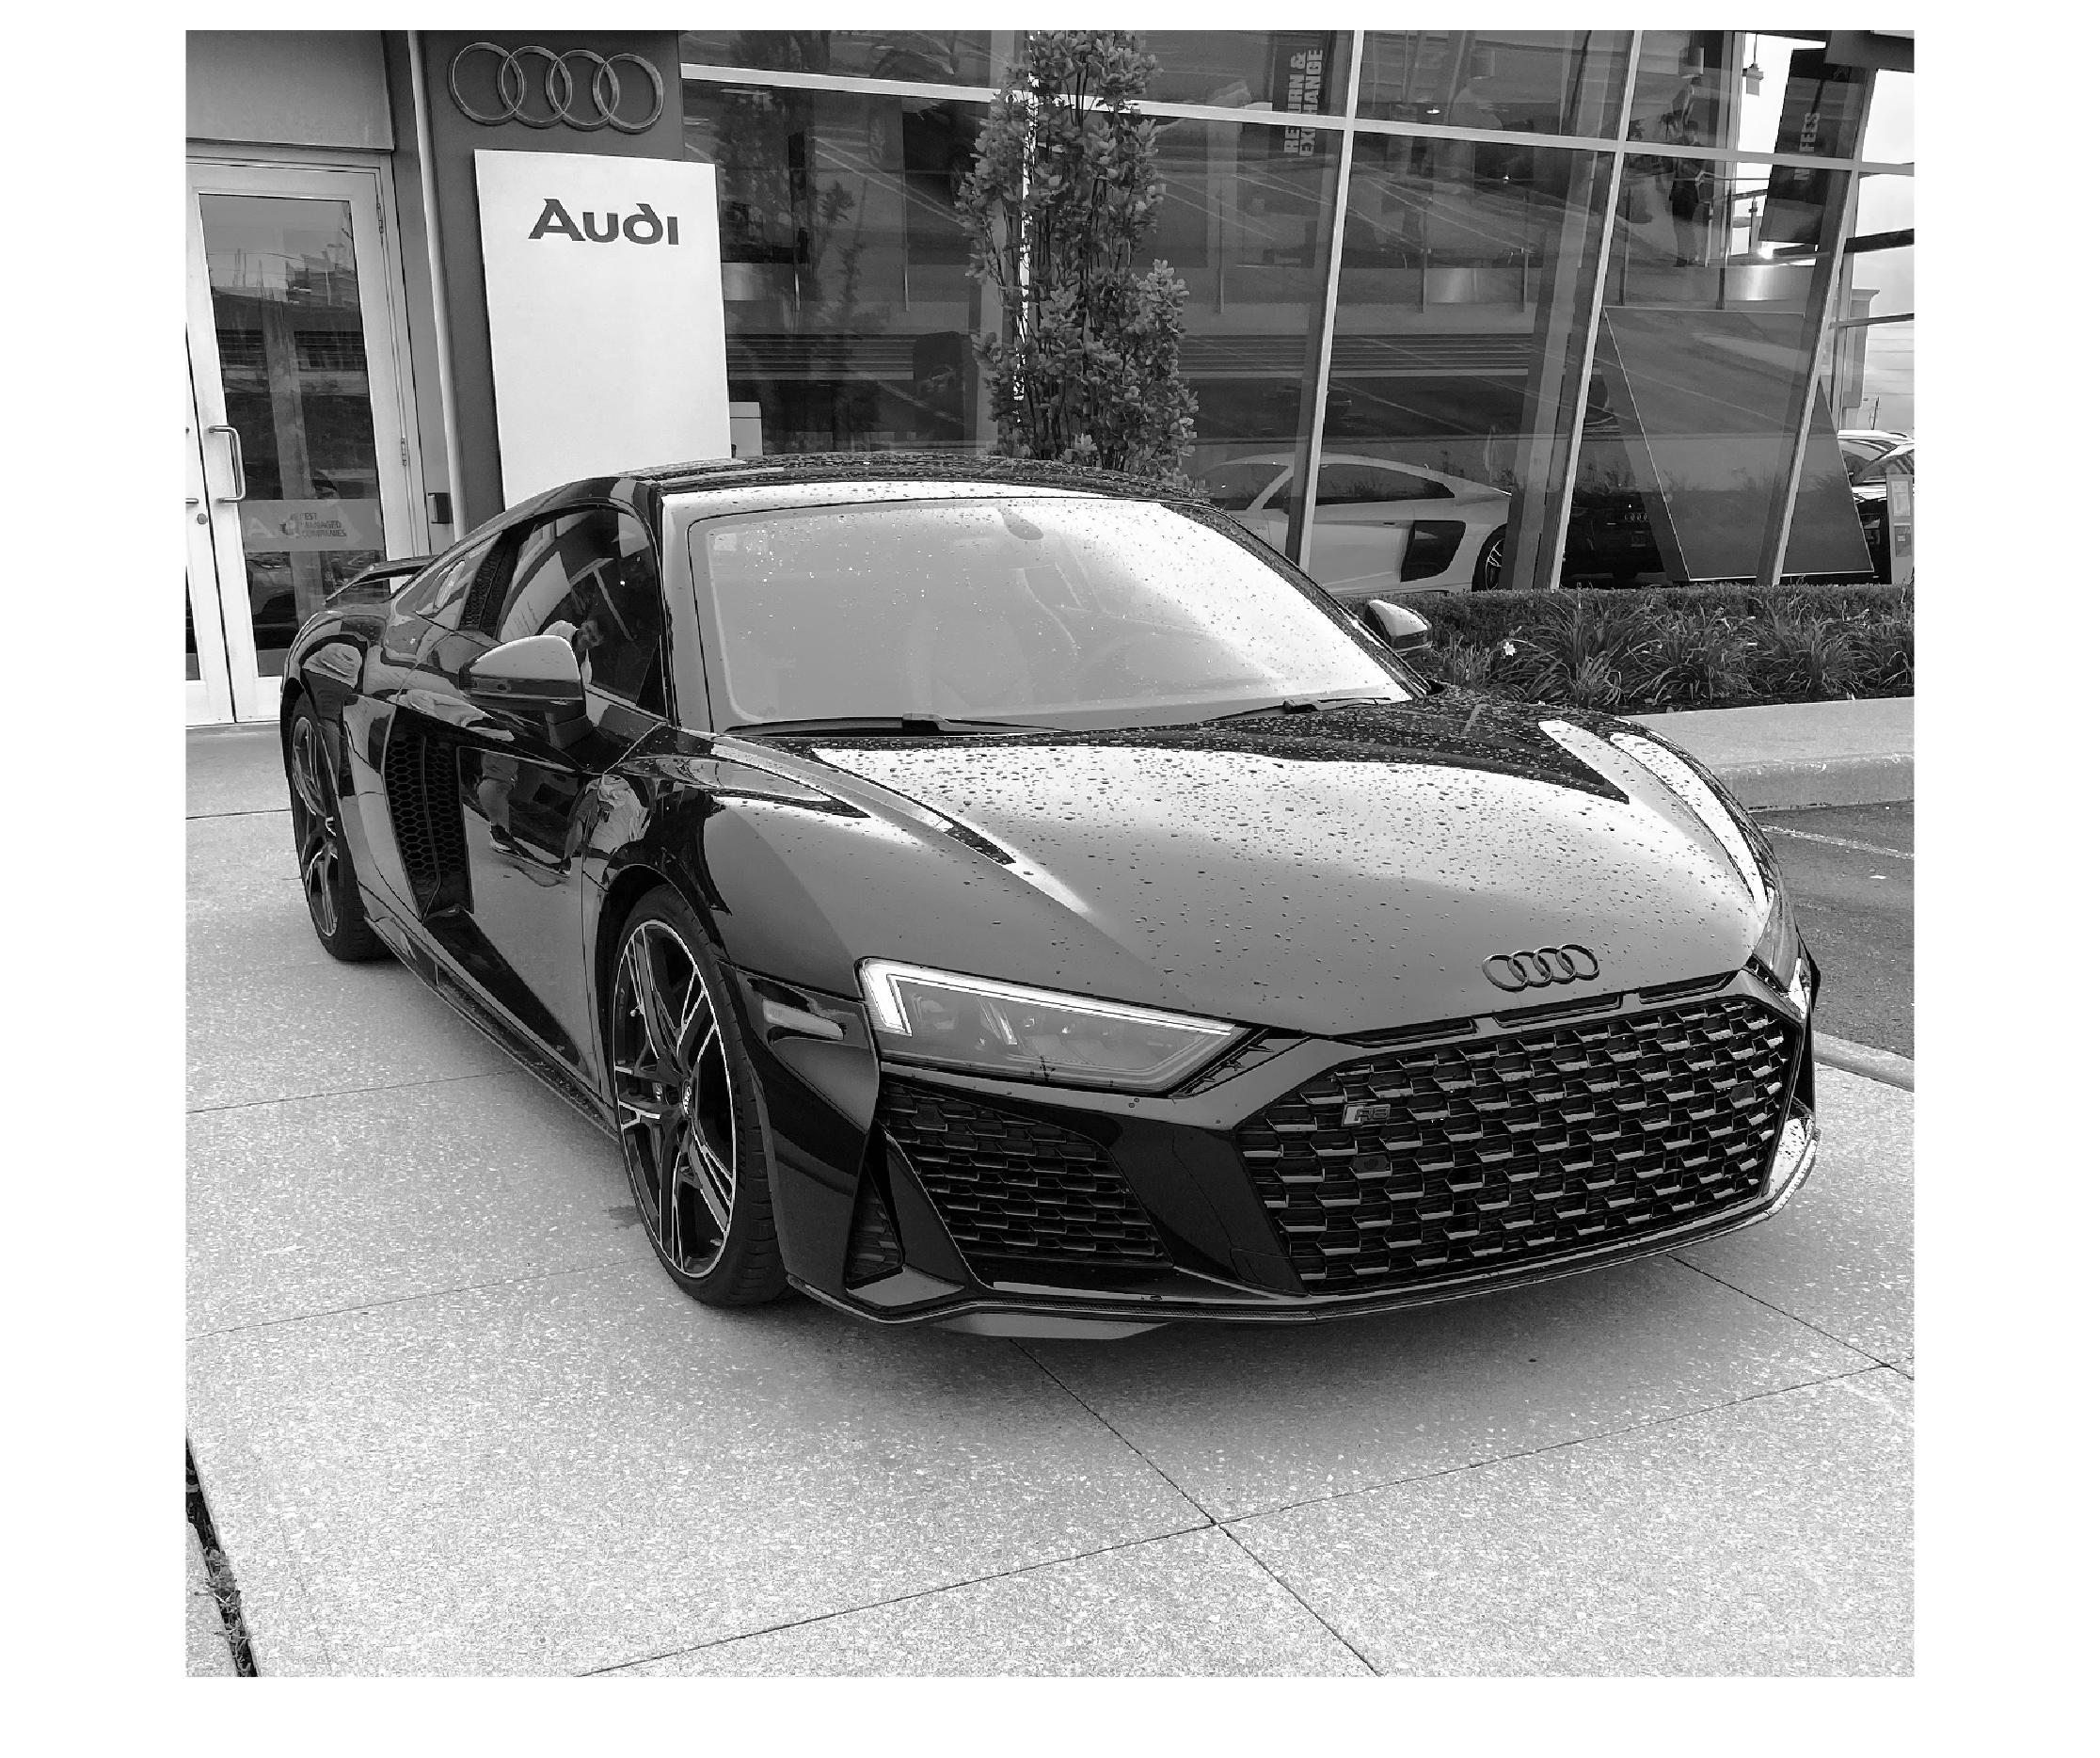
\includegraphics[width=\linewidth]{images/img14.jpg}
\caption{After equalization)}
\end{subfigure}
\begin{subfigure}[b]{0.4\linewidth}
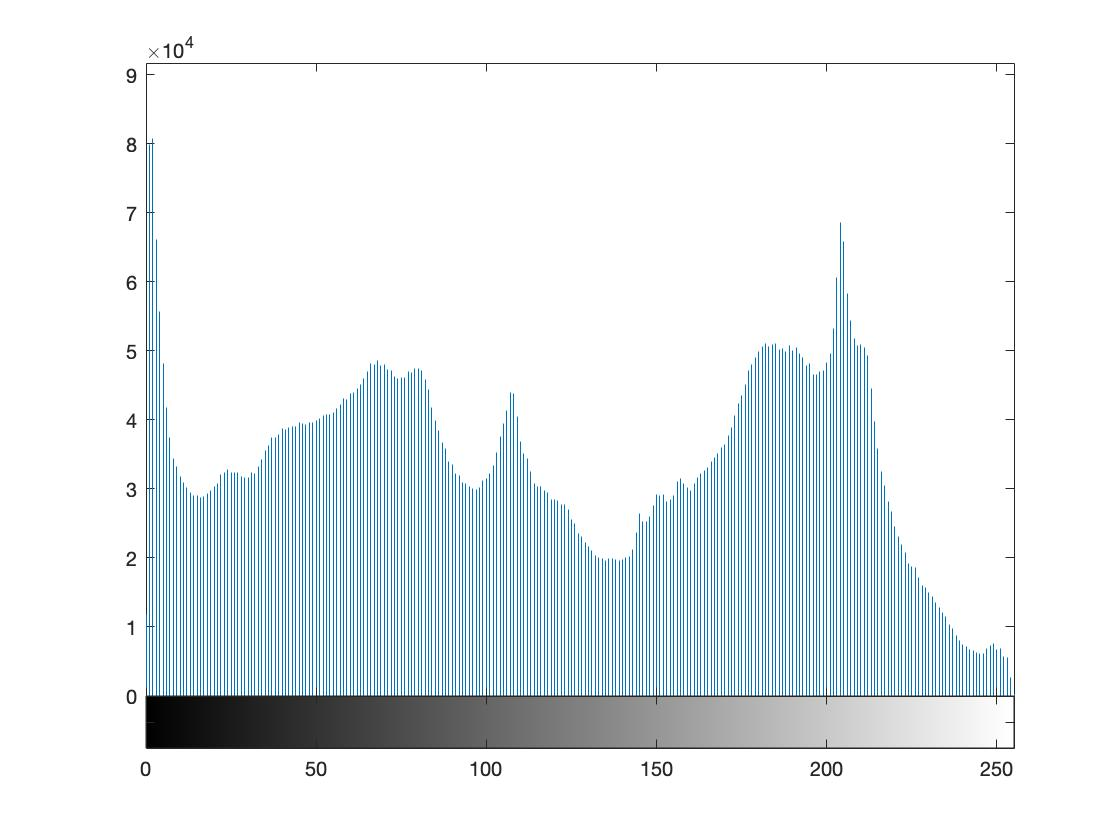
\includegraphics[width=\linewidth]{images/img15.jpg}
\caption{Before equalization}
\end{subfigure}
\begin{subfigure}[b]{0.4\linewidth}
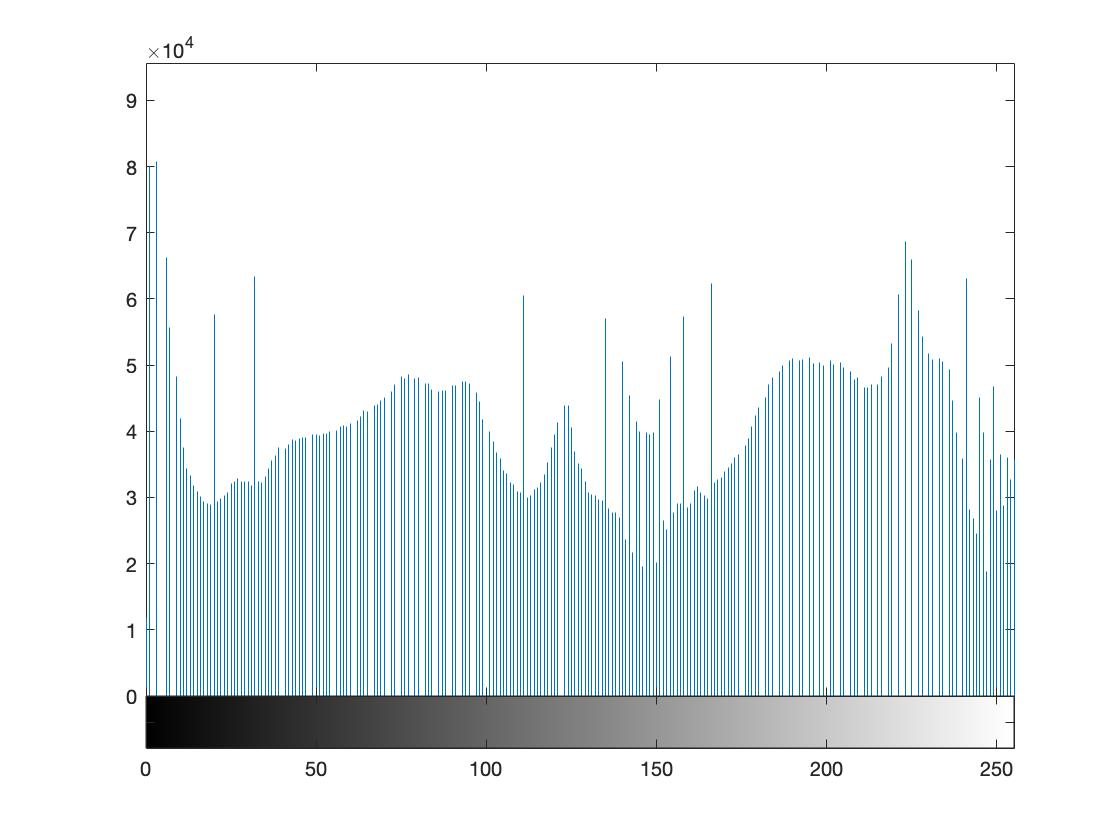
\includegraphics[width=\linewidth]{images/img16.jpg}
\caption{After equalization}
\end{subfigure}
\caption{Grayscale image histogram equalization results}
\label{fig:Grayscale image histogram equalization results}
\end{figure}

\begin{figure}[h!]
\centering
\begin{subfigure}[b]{0.4\linewidth}
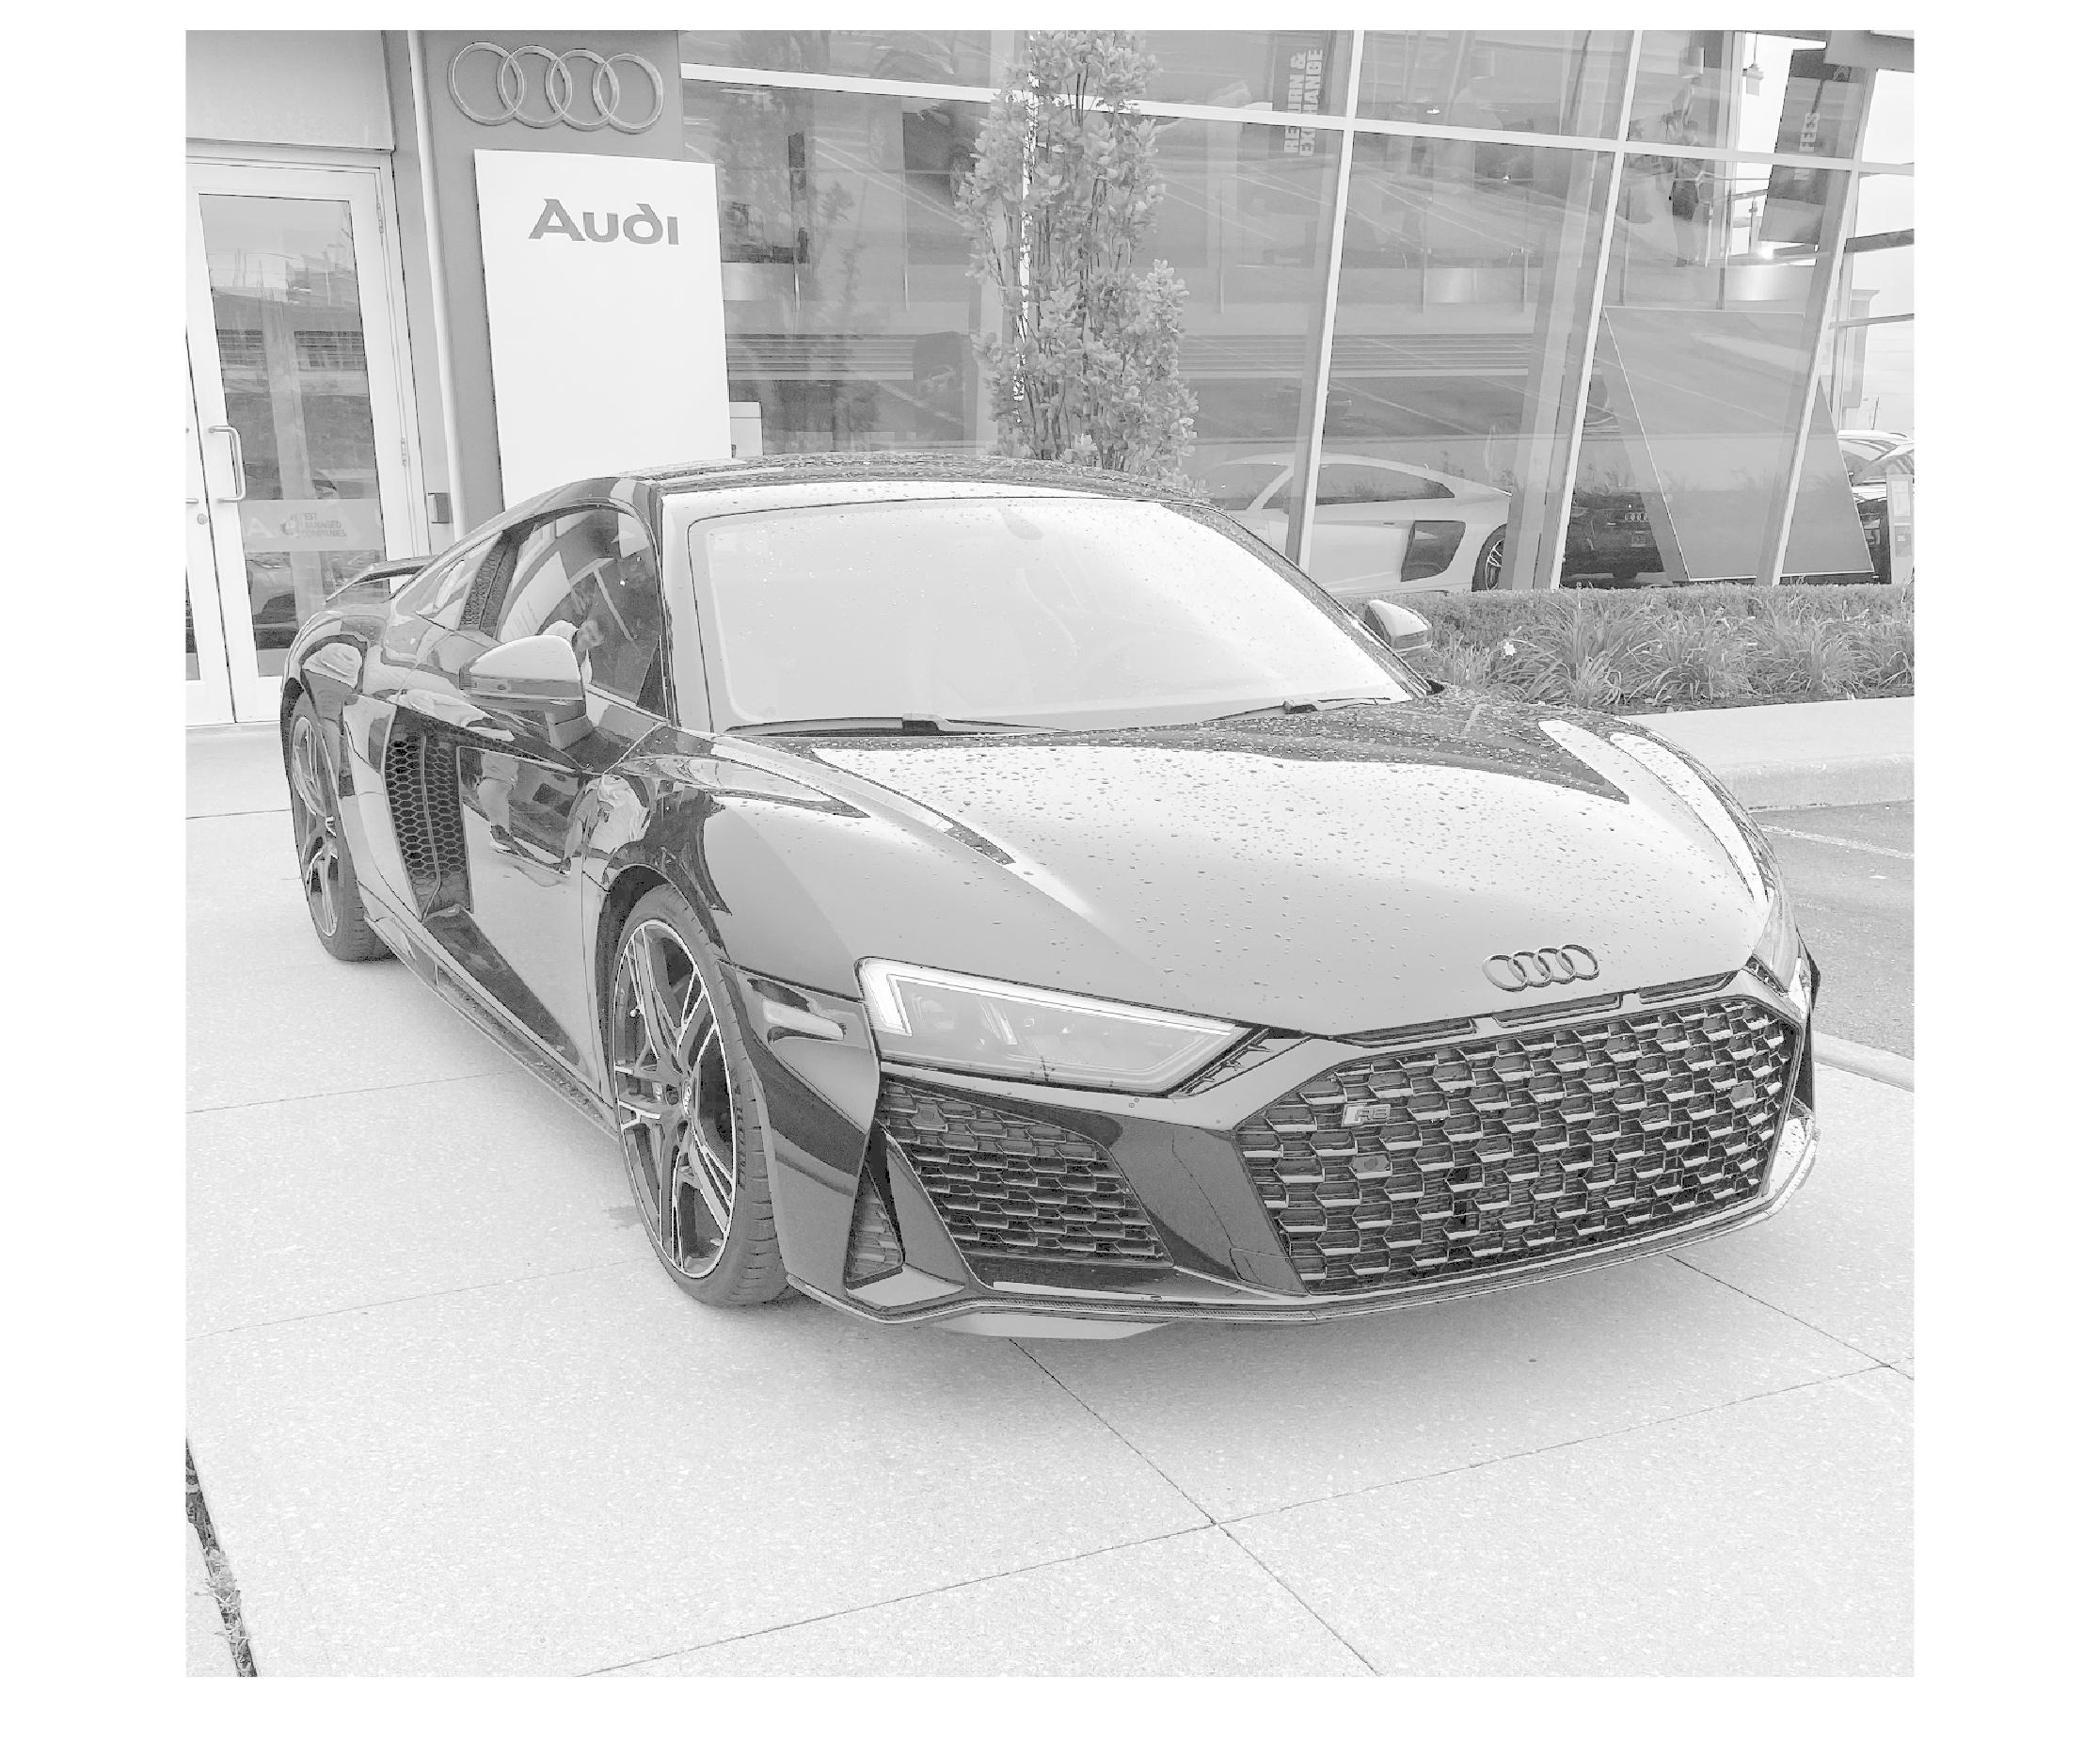
\includegraphics[width=\linewidth]{images/img2.jpg}
\caption{Before equalization}
\end{subfigure}
\begin{subfigure}[b]{0.4\linewidth}
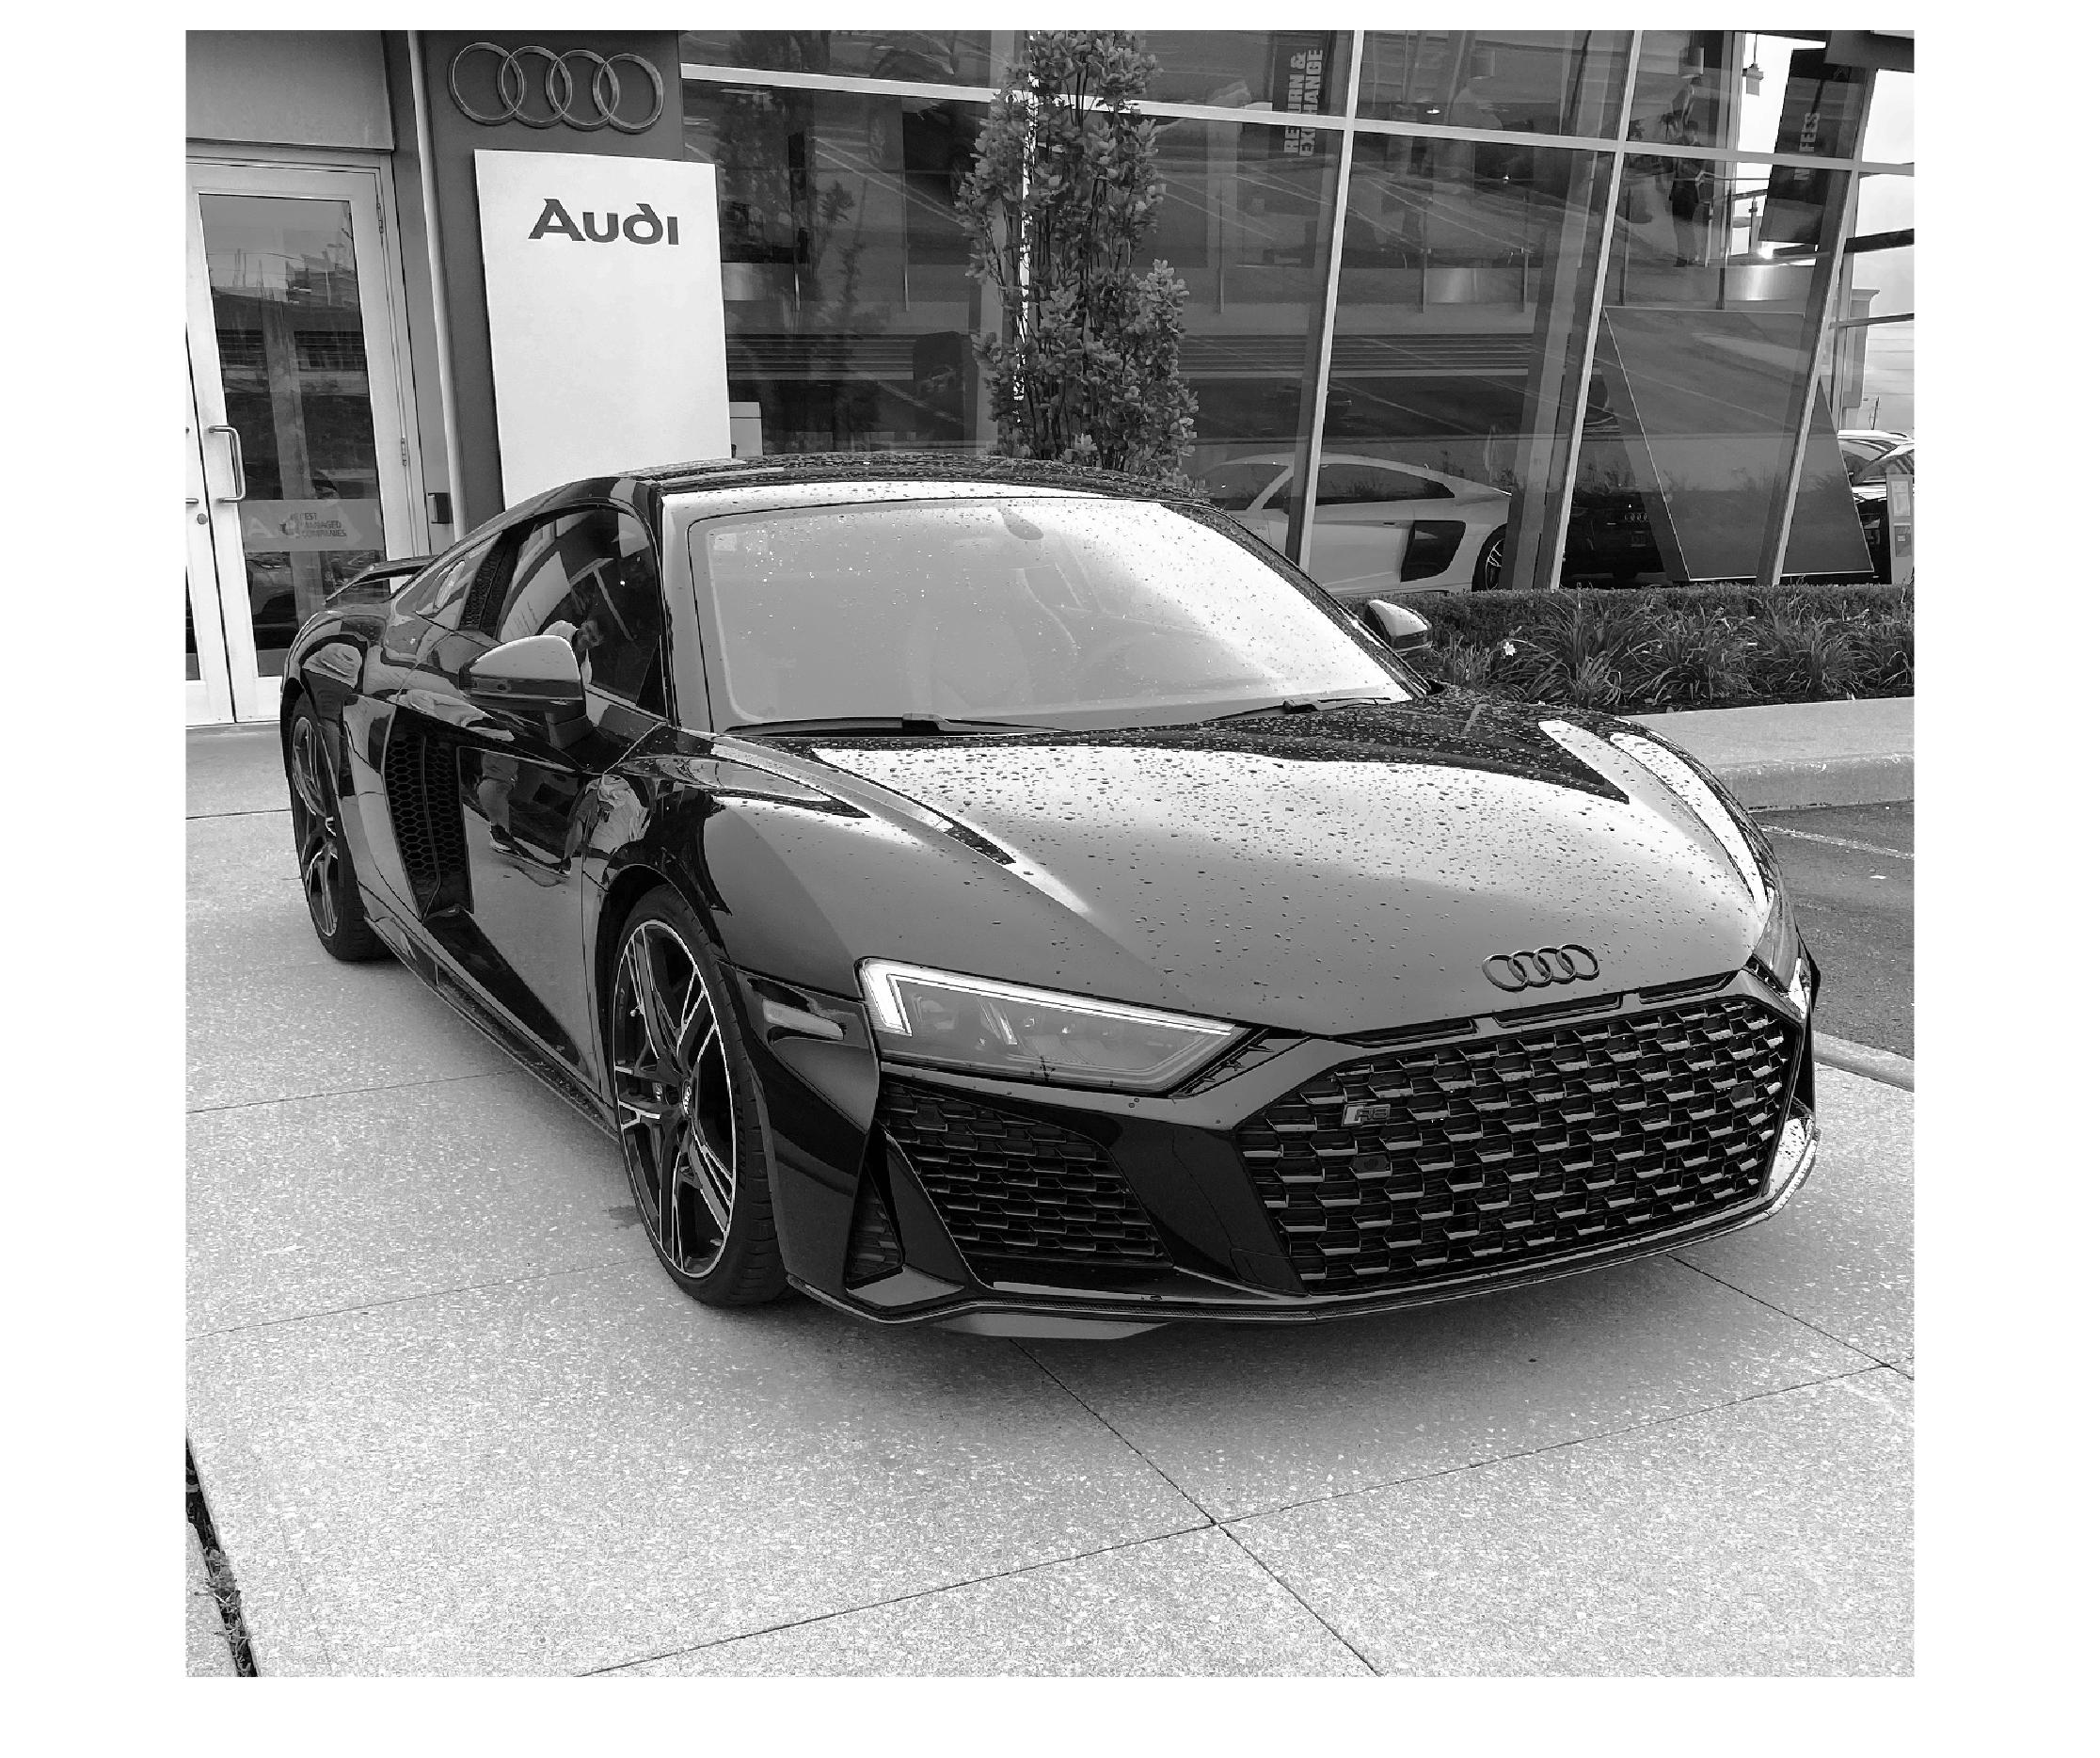
\includegraphics[width=\linewidth]{images/img17.jpg}
\caption{After equalization)}
\end{subfigure}
\begin{subfigure}[b]{0.4\linewidth}
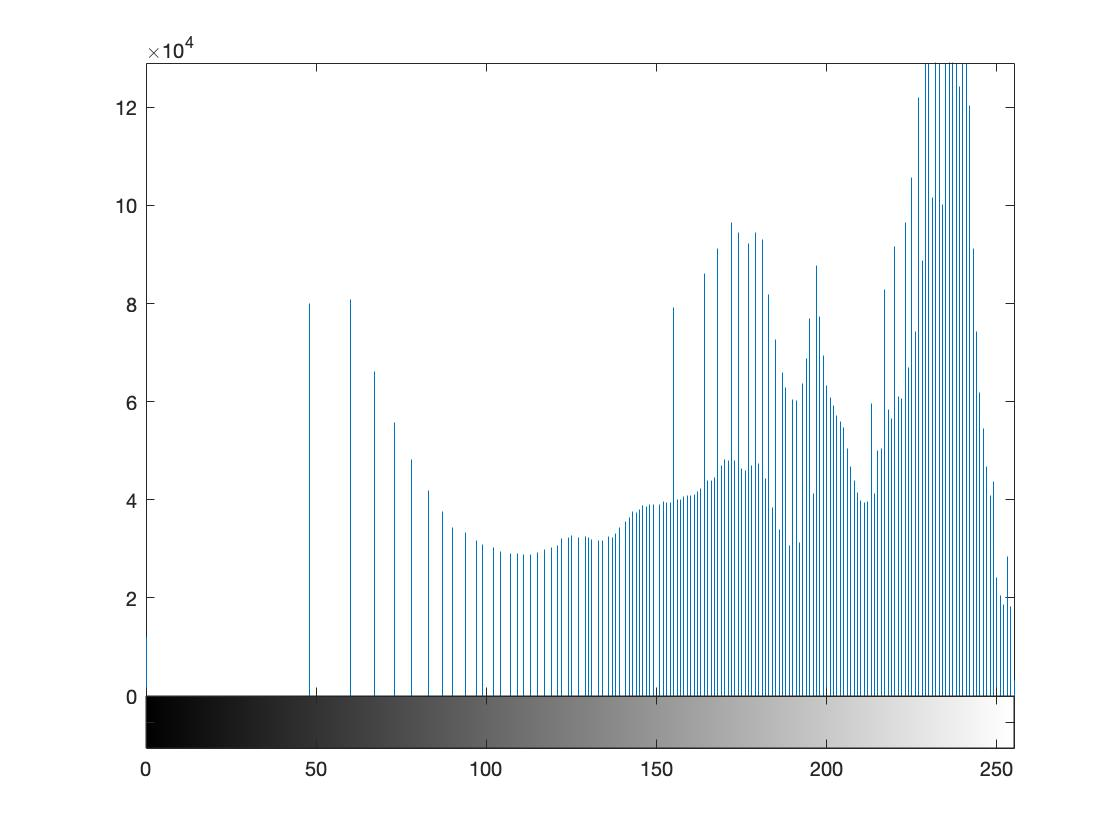
\includegraphics[width=\linewidth]{images/img18.jpg}
\caption{Before equalization}
\end{subfigure}
\begin{subfigure}[b]{0.4\linewidth}
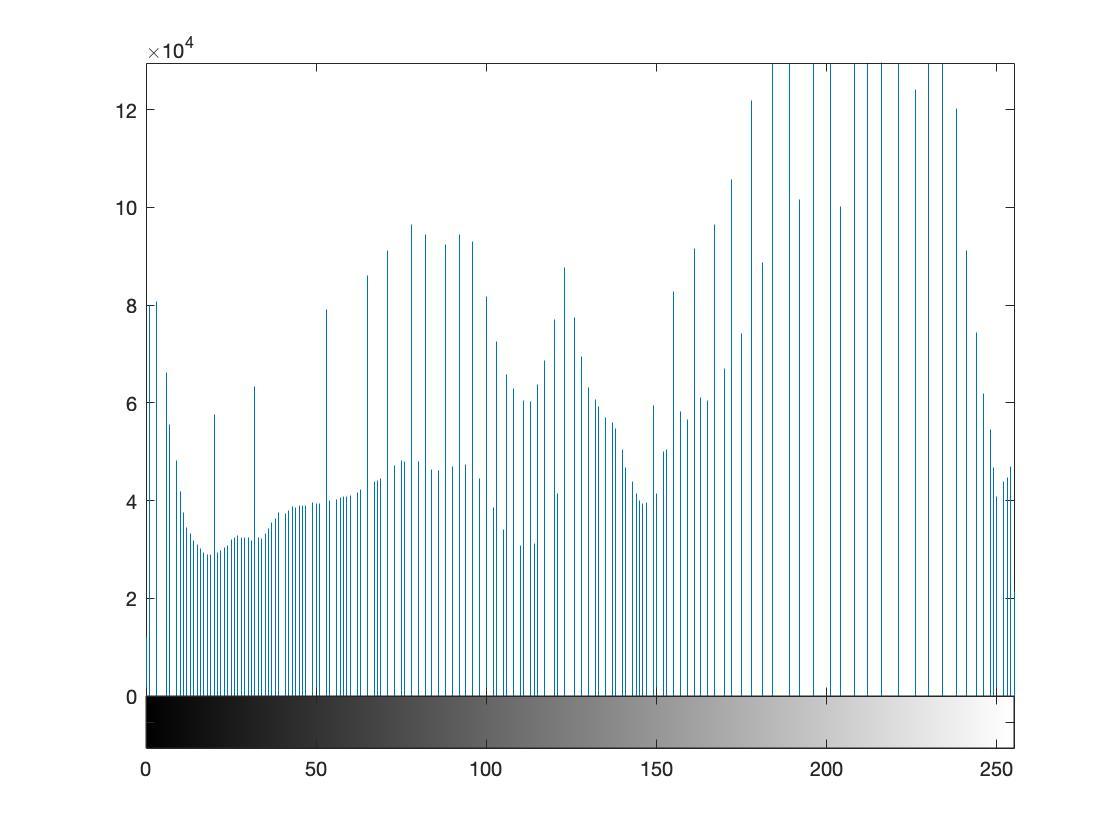
\includegraphics[width=\linewidth]{images/img19.jpg}
\caption{After equalization}
\end{subfigure}
\caption{\(\gamma = 0.3\) image histogram equalization results}
\label{fig:b}
\end{figure}

\begin{figure}[h!]
\centering
\begin{subfigure}[b]{0.4\linewidth}
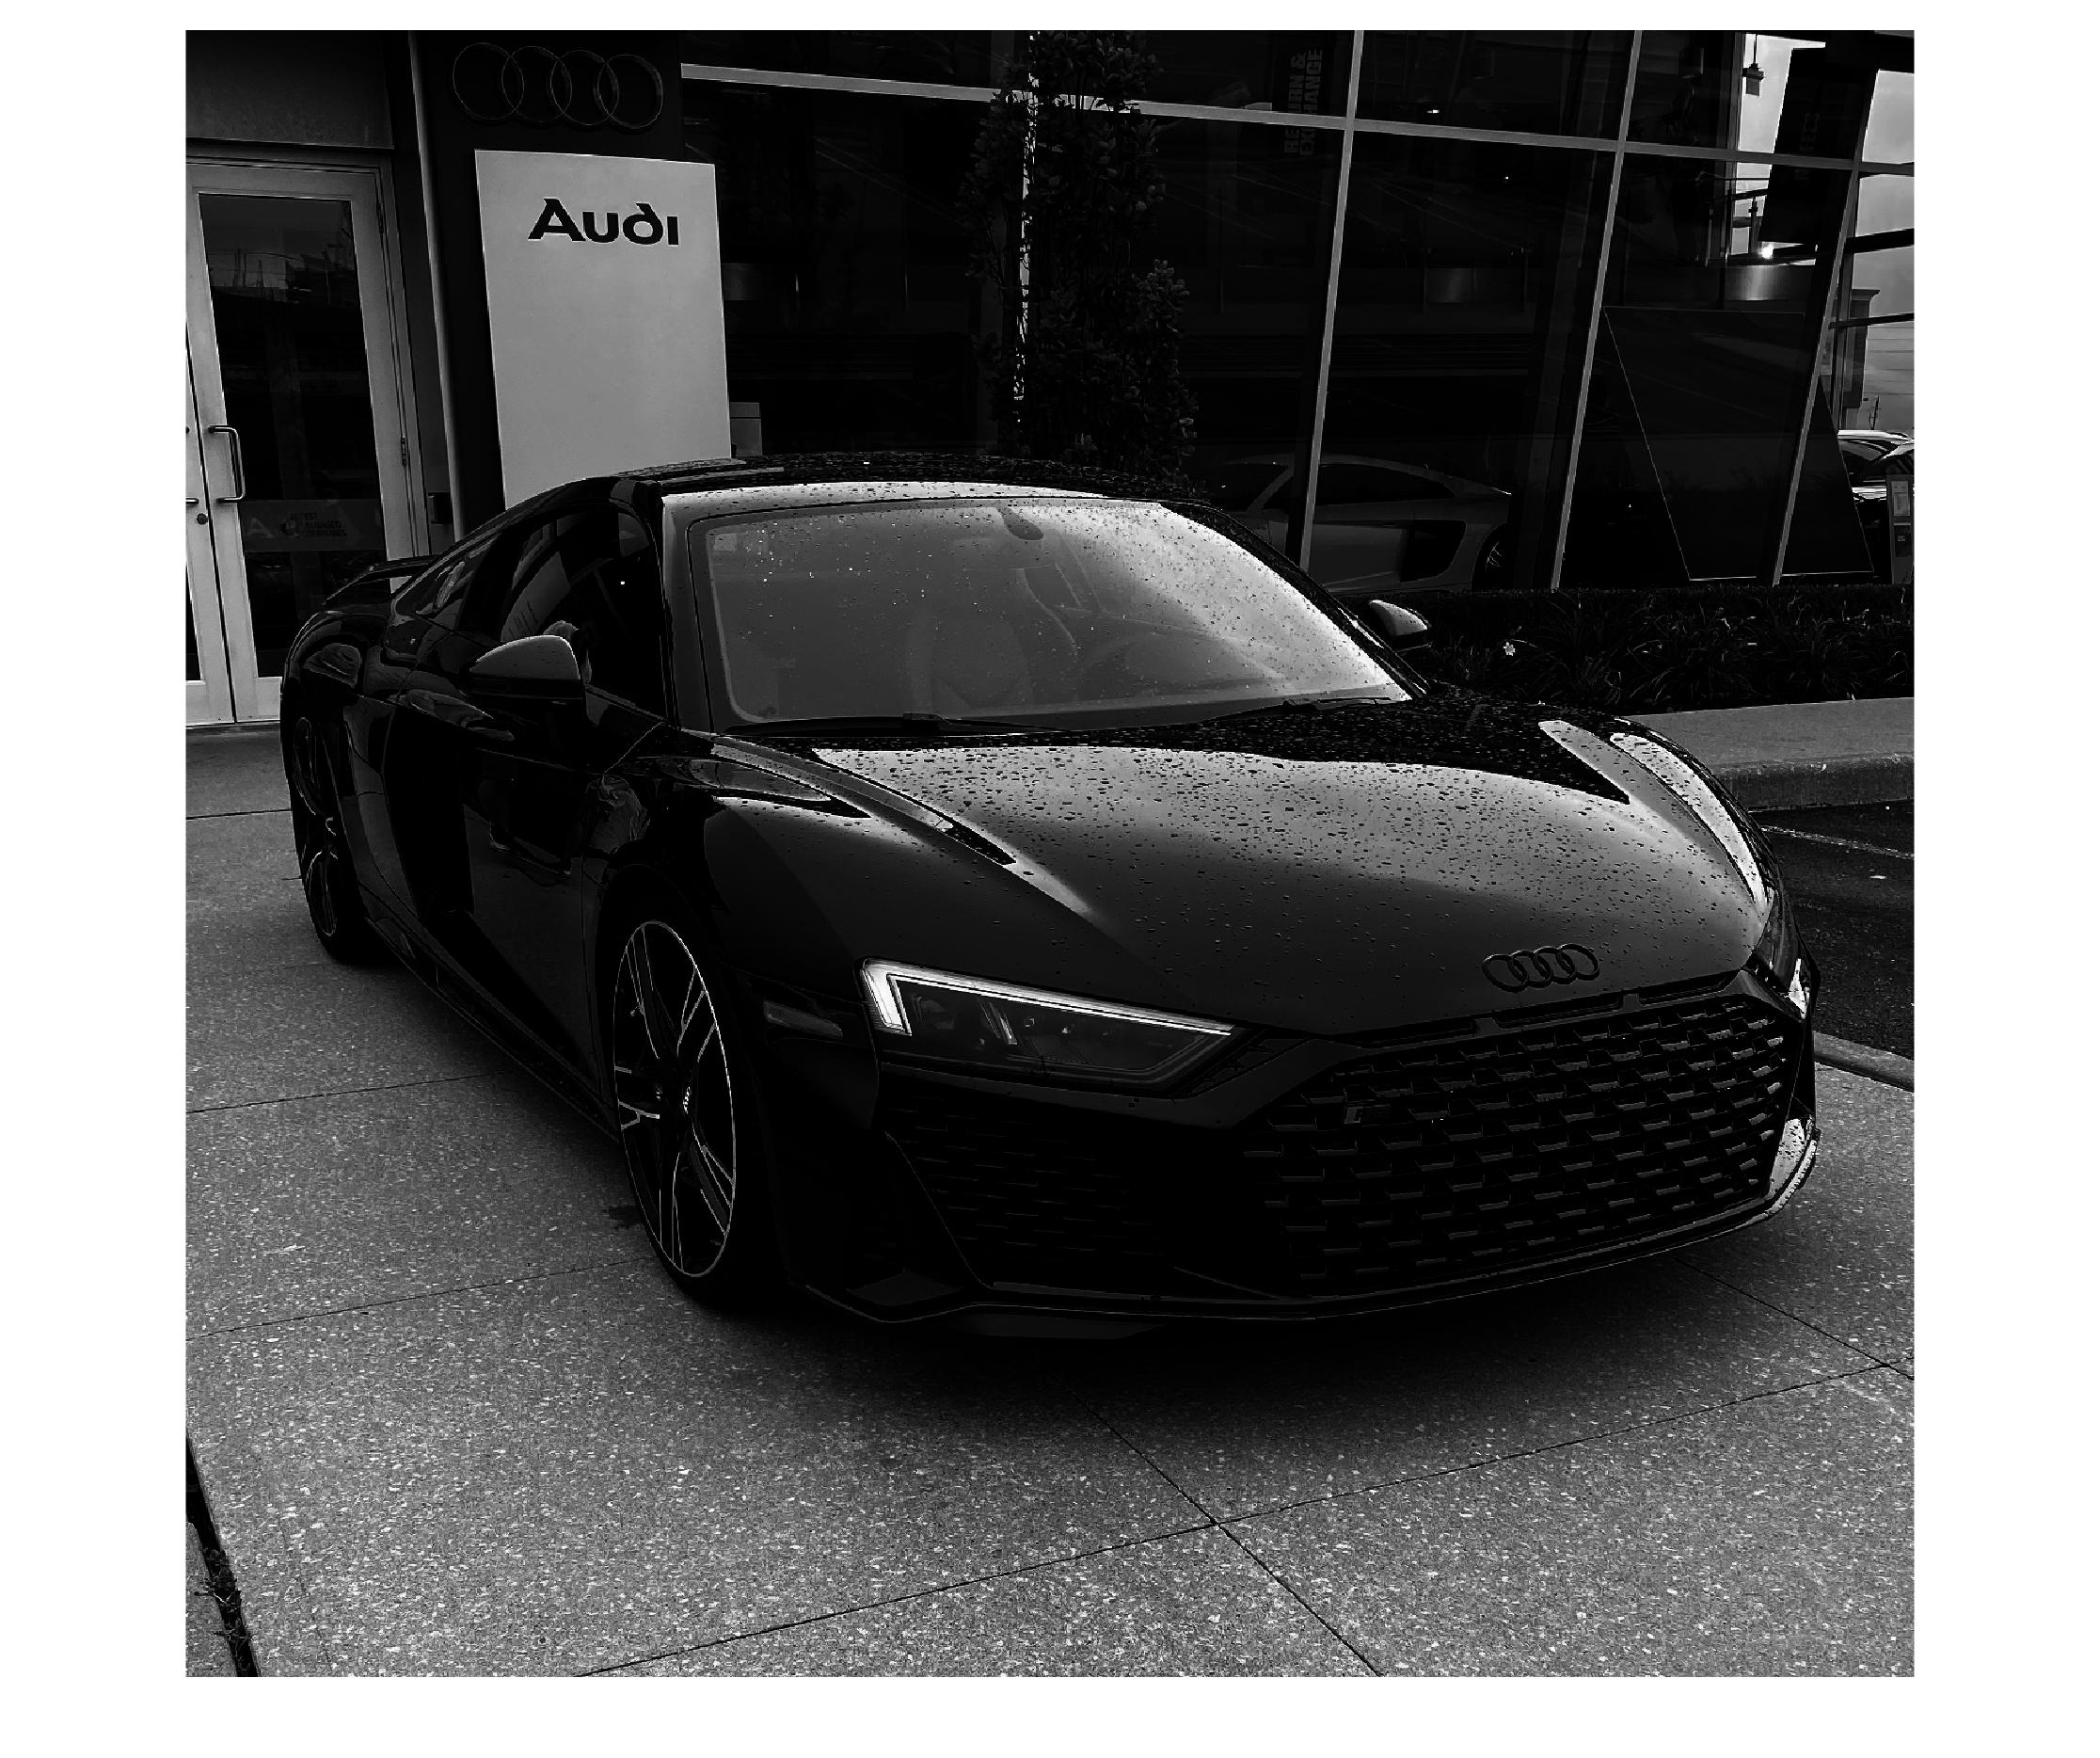
\includegraphics[width=\linewidth]{images/img3.jpg}
\caption{Before equalization}
\end{subfigure}
\begin{subfigure}[b]{0.4\linewidth}
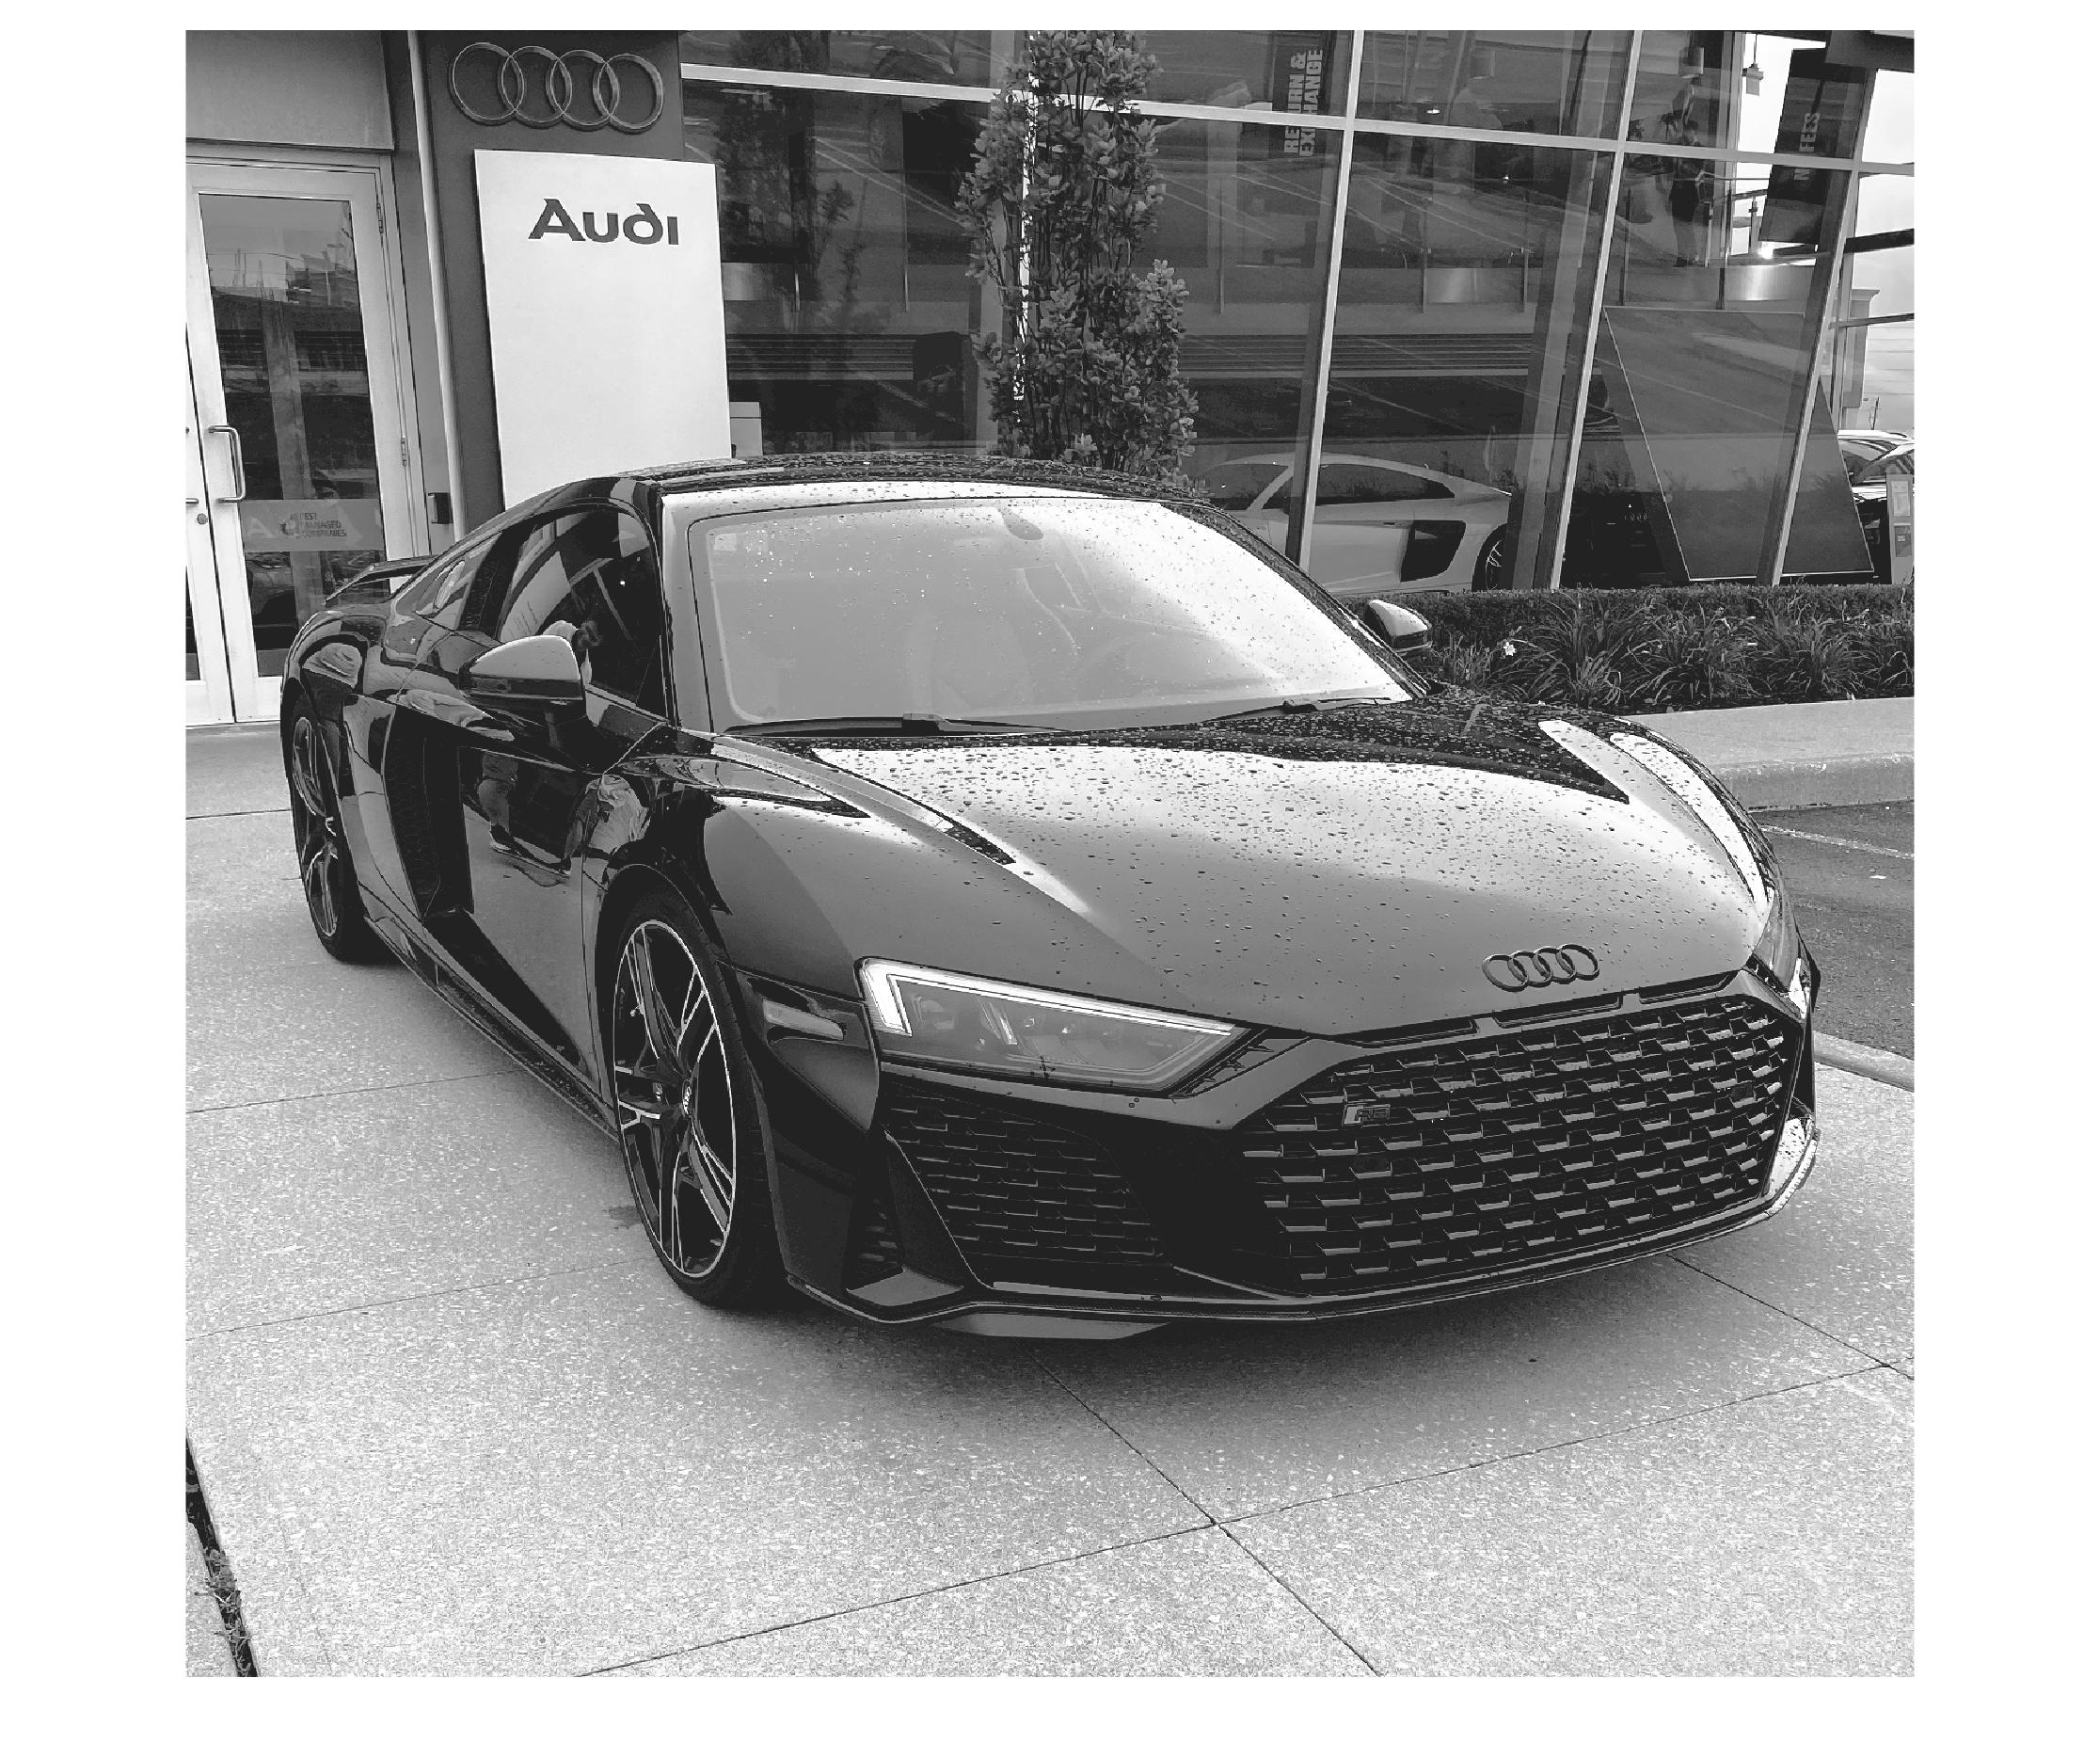
\includegraphics[width=\linewidth]{images/img20.jpg}
\caption{After equalization}
\end{subfigure}
\begin{subfigure}[b]{0.4\linewidth}
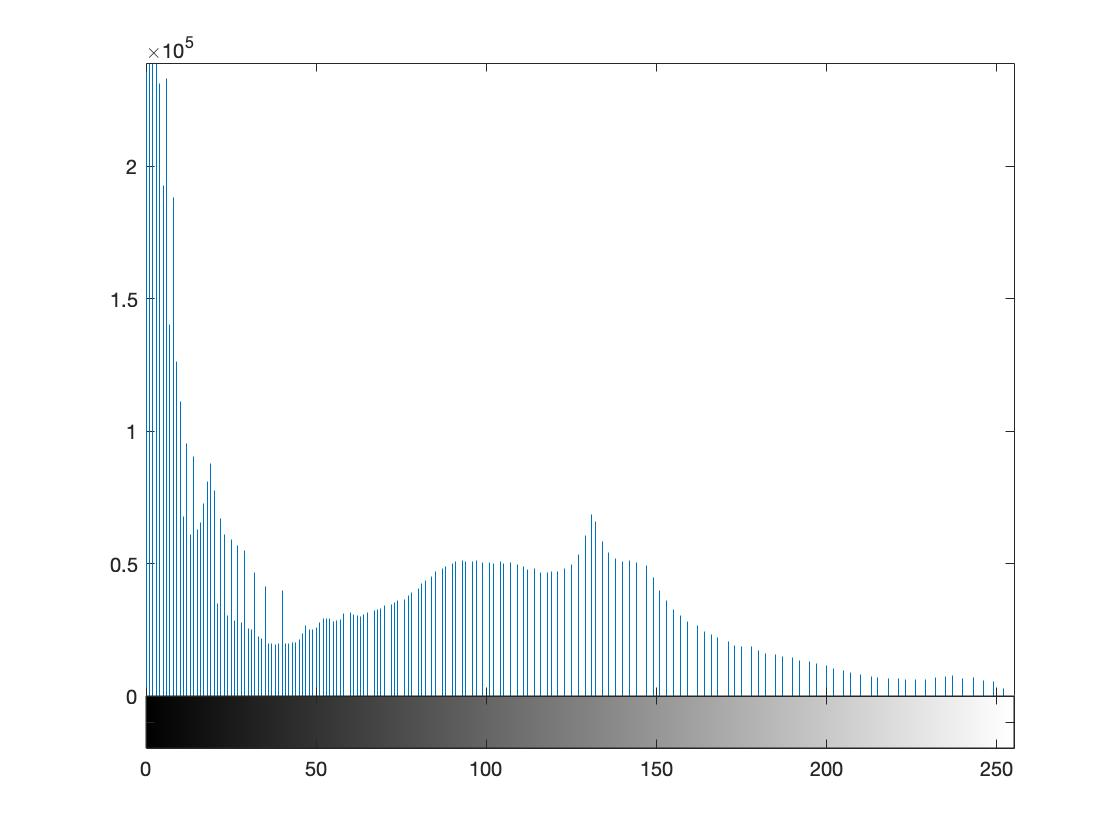
\includegraphics[width=\linewidth]{images/img21.jpg}
\caption{Before equalization}
\end{subfigure}
\begin{subfigure}[b]{0.4\linewidth}
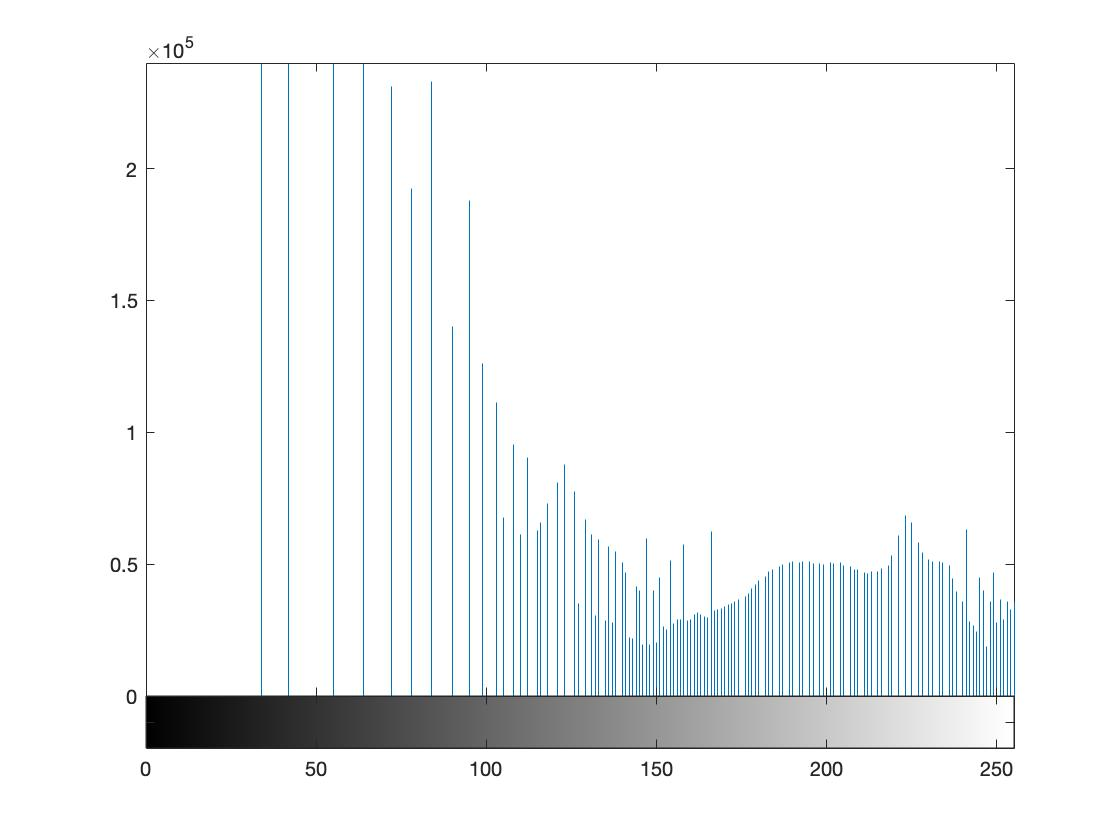
\includegraphics[width=\linewidth]{images/img22.jpg}
\caption{After equalization}
\end{subfigure}
\caption{\(\gamma = 3\) image histogram equalization results}
\label{fig:a}
\end{figure}

\clearpage
\subsection{Problem 4}
Histogram matching (specification) is a quick and easy way to "calibrate" one image to match another. In mathematical terms, it's the process of transforming one image so that the cumulative distribution function (CDF) of values in each band matches the CDF of bands in another image.

The process of histogram matching can be specified as follow:
\begin{description}[font=$\bullet$~\normalfont\scshape\color{red!50!black}]
  \item Compute histogram of the input images \(p_r(r)\) and the histogram equalized image \(s = T(r)\)
  \item Compute \(s = G(z)\) where G is the equalization function derived from a specified histogram
  \item Perform the inverse mapping \(z = G^{-1}(s)\)
  \item The output image with \(z\) values is then of the specified histogram
\end{description}

For a real image, with 8-bit pixel values (discrete values in range [0, 255]), histogram matching can only approximate the specified histogram. All pixels of a particular value in the original image must be transformed to just one value in the output image. There are various methods have been proposed for exact histogram matching but they cause noise to the output image. Therefore, the desired histogram cannot be obtained after histogram matching.

\subsection{Problem 5}

Compute of the histogram for the following 3-bit image:

\begin{figure}[h!]
\centering
\begin{subfigure}[b]{0.4\linewidth}
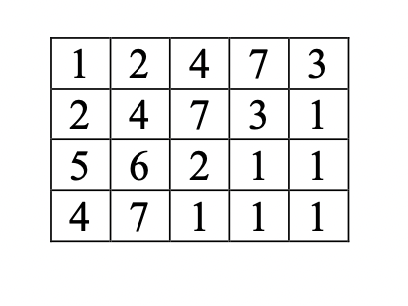
\includegraphics[width=\linewidth]{images/img24.jpg}
\caption{3-bit image}
\end{subfigure}
\begin{subfigure}[b]{0.4\linewidth}
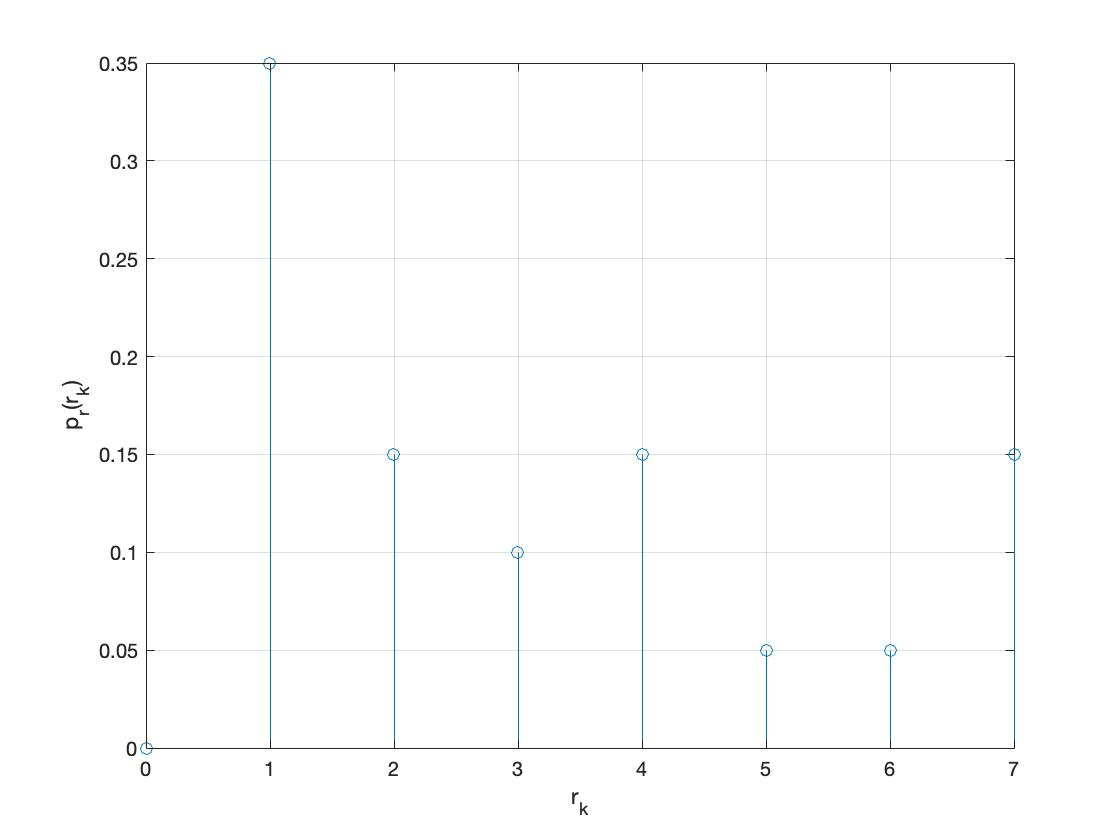
\includegraphics[width=\linewidth]{images/img23.jpg}
\caption{Intensity distribution}
\end{subfigure}
\caption{3-bit image and its intensity distribution}
\label{fig: Intensity distribution}
\end{figure}

Sample calculation:
\[p_r(r_k)=n_k/MN\]
\[p_r(r_1)=7/20=0.35\]

\begin{table}[h!]
\centering
\begin{tabular}{|| c c c||} 
 \hline
 \(r_k\)  & \(n_k\) & \(p_r(r_k)=n_k/MN\) \\ [0.5ex] 
 \hline\hline
 \(r_0=0\) & 0 & 0 \\ 
 \hline
 \(r_1=1\)& 7 & 0.35 \\
 \hline
 \(r_2=2\)& 3 & 0.15 \\
 \hline
 \(r_3=3\)& 2 & 0.1 \\
 \hline
 \(r_4=4\)& 3 & 0.15 \\ 
 \hline
 \(r_5=5\)& 1 & 0.05 \\
 \hline
 \(r_6=6\)& 1 & 0.05 \\
 \hline
 \(r_7=7\)& 3 & 0.15 \\
 \hline
\end{tabular}
\caption{Intensity distribution and histogram values}
\label{table:1}
\end{table}

Sample calculation:
\[ s_0 = T(r_0) = 7\sum_{j=0}^{0} p_r(r_j) = 7p_r(r_0) = 0 \]
\[ s_1 = T(r_1) = 7\sum_{j=1}^{0} p_r(r_j) = 7p_r(r_0) + 7p_r(r_1) = 2.45\]
Similarly,
\[s_2=3.5,  s_3=4.2,    s_4=5.25,\]
\[s_5=5.6,  s_6=5.95,   s_7=7.0\]

We round the s values to get the equalized histogram,
\[s_0=0 \rightarrow 0, s_1=2.45 \rightarrow 2, s_2=3.5 \rightarrow 4, s_3=4.2 \rightarrow 4,\]
\[s_4=5.25 \rightarrow 5, s_5=5.6 \rightarrow 6,  s_6=5.95 \rightarrow 6,   s_7=7.0 \rightarrow 7\]

The new image is as follow:

\begin{tabularx}{0.2\textwidth} { 
  | >{\centering\arraybackslash}X
  | >{\centering\arraybackslash}X
  | >{\centering\arraybackslash}X
  | >{\centering\arraybackslash}X 
  | >{\centering\arraybackslash}X | }
 \hline
 2 & 4 & 5 & 7 & 4 \\
 \hline
 4 & 5 & 7 & 4 & 2 \\
 \hline
 6 & 6 & 4 & 2 & 2 \\
 \hline
 5 & 7 & 2 & 2 & 2 \\
\hline
\end{tabularx}

The histogram after equalization is shown below:
\begin{figure}[h!]
\centering
\begin{subfigure}[b]{0.4\linewidth}
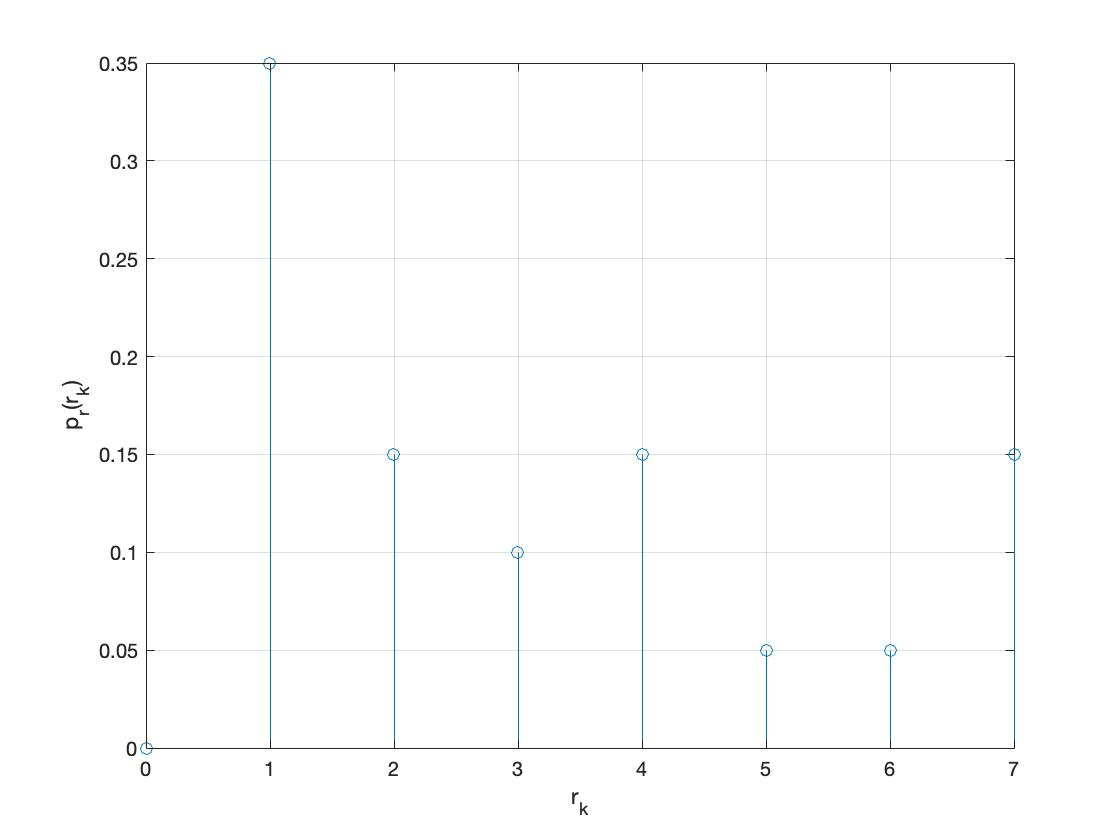
\includegraphics[width=\linewidth]{images/img23.jpg}
\caption{Original histogram}
\end{subfigure}
\begin{subfigure}[b]{0.4\linewidth}
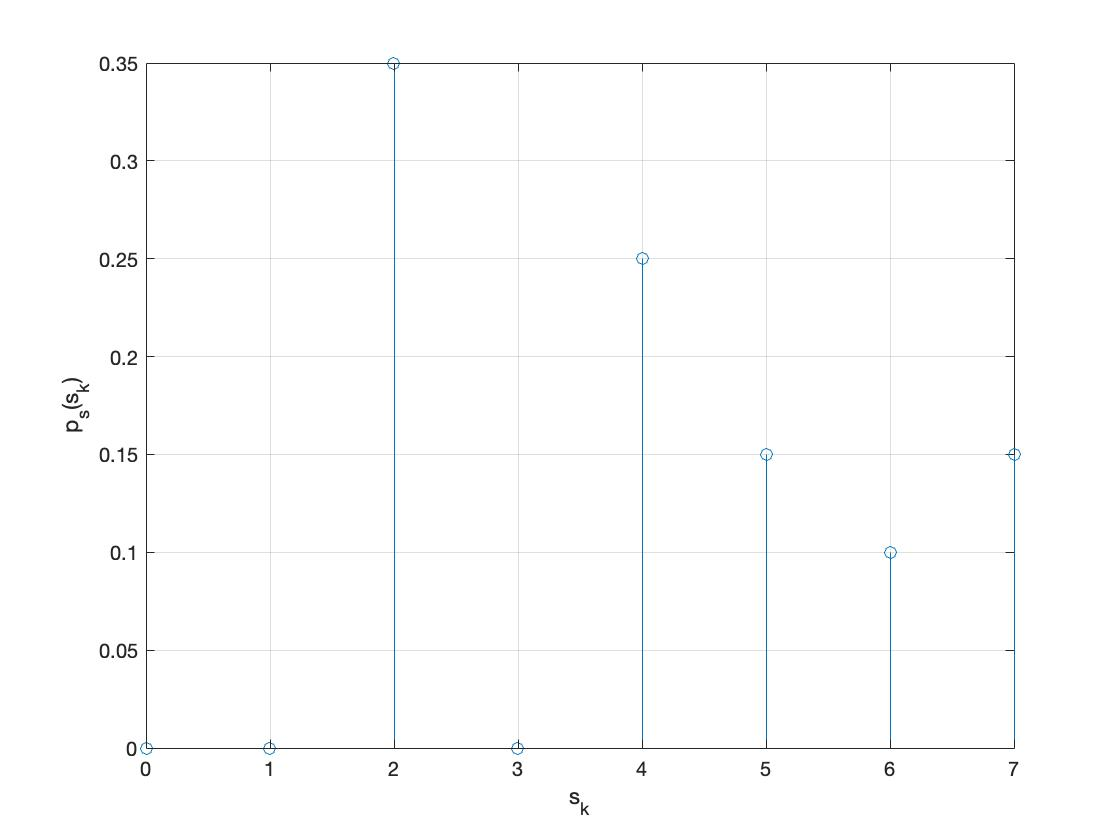
\includegraphics[width=\linewidth]{images/img25.jpg}
\caption{Equalized histogram}
\end{subfigure}
\caption{Histogram equalization of 3-bit image}
\label{fig: Histogram equalization of 3-bit image}
\end{figure}

\clearpage
\section{Part 2}

\subsection{Transform an Image Using Simple Shear}
\begin{lstlisting}[language=Matlab]
% Step 1: Transform an Image 
% Using Simple Shear
% Set a value
a = 0.45;
% Construct an affine tform struct 
% using maketform
T=maketform('affine',
        [1 0 0; a 1 0; 0 0 1]);

% Load and display image
img = imread('/lamnguyen/Desktop/School/
Computer-Vision/A1/images/bear.jpg');
h1 = figure;
imshow(img)
title('Original Image')
\end{lstlisting}

\begin{figure}[h!]
\centering
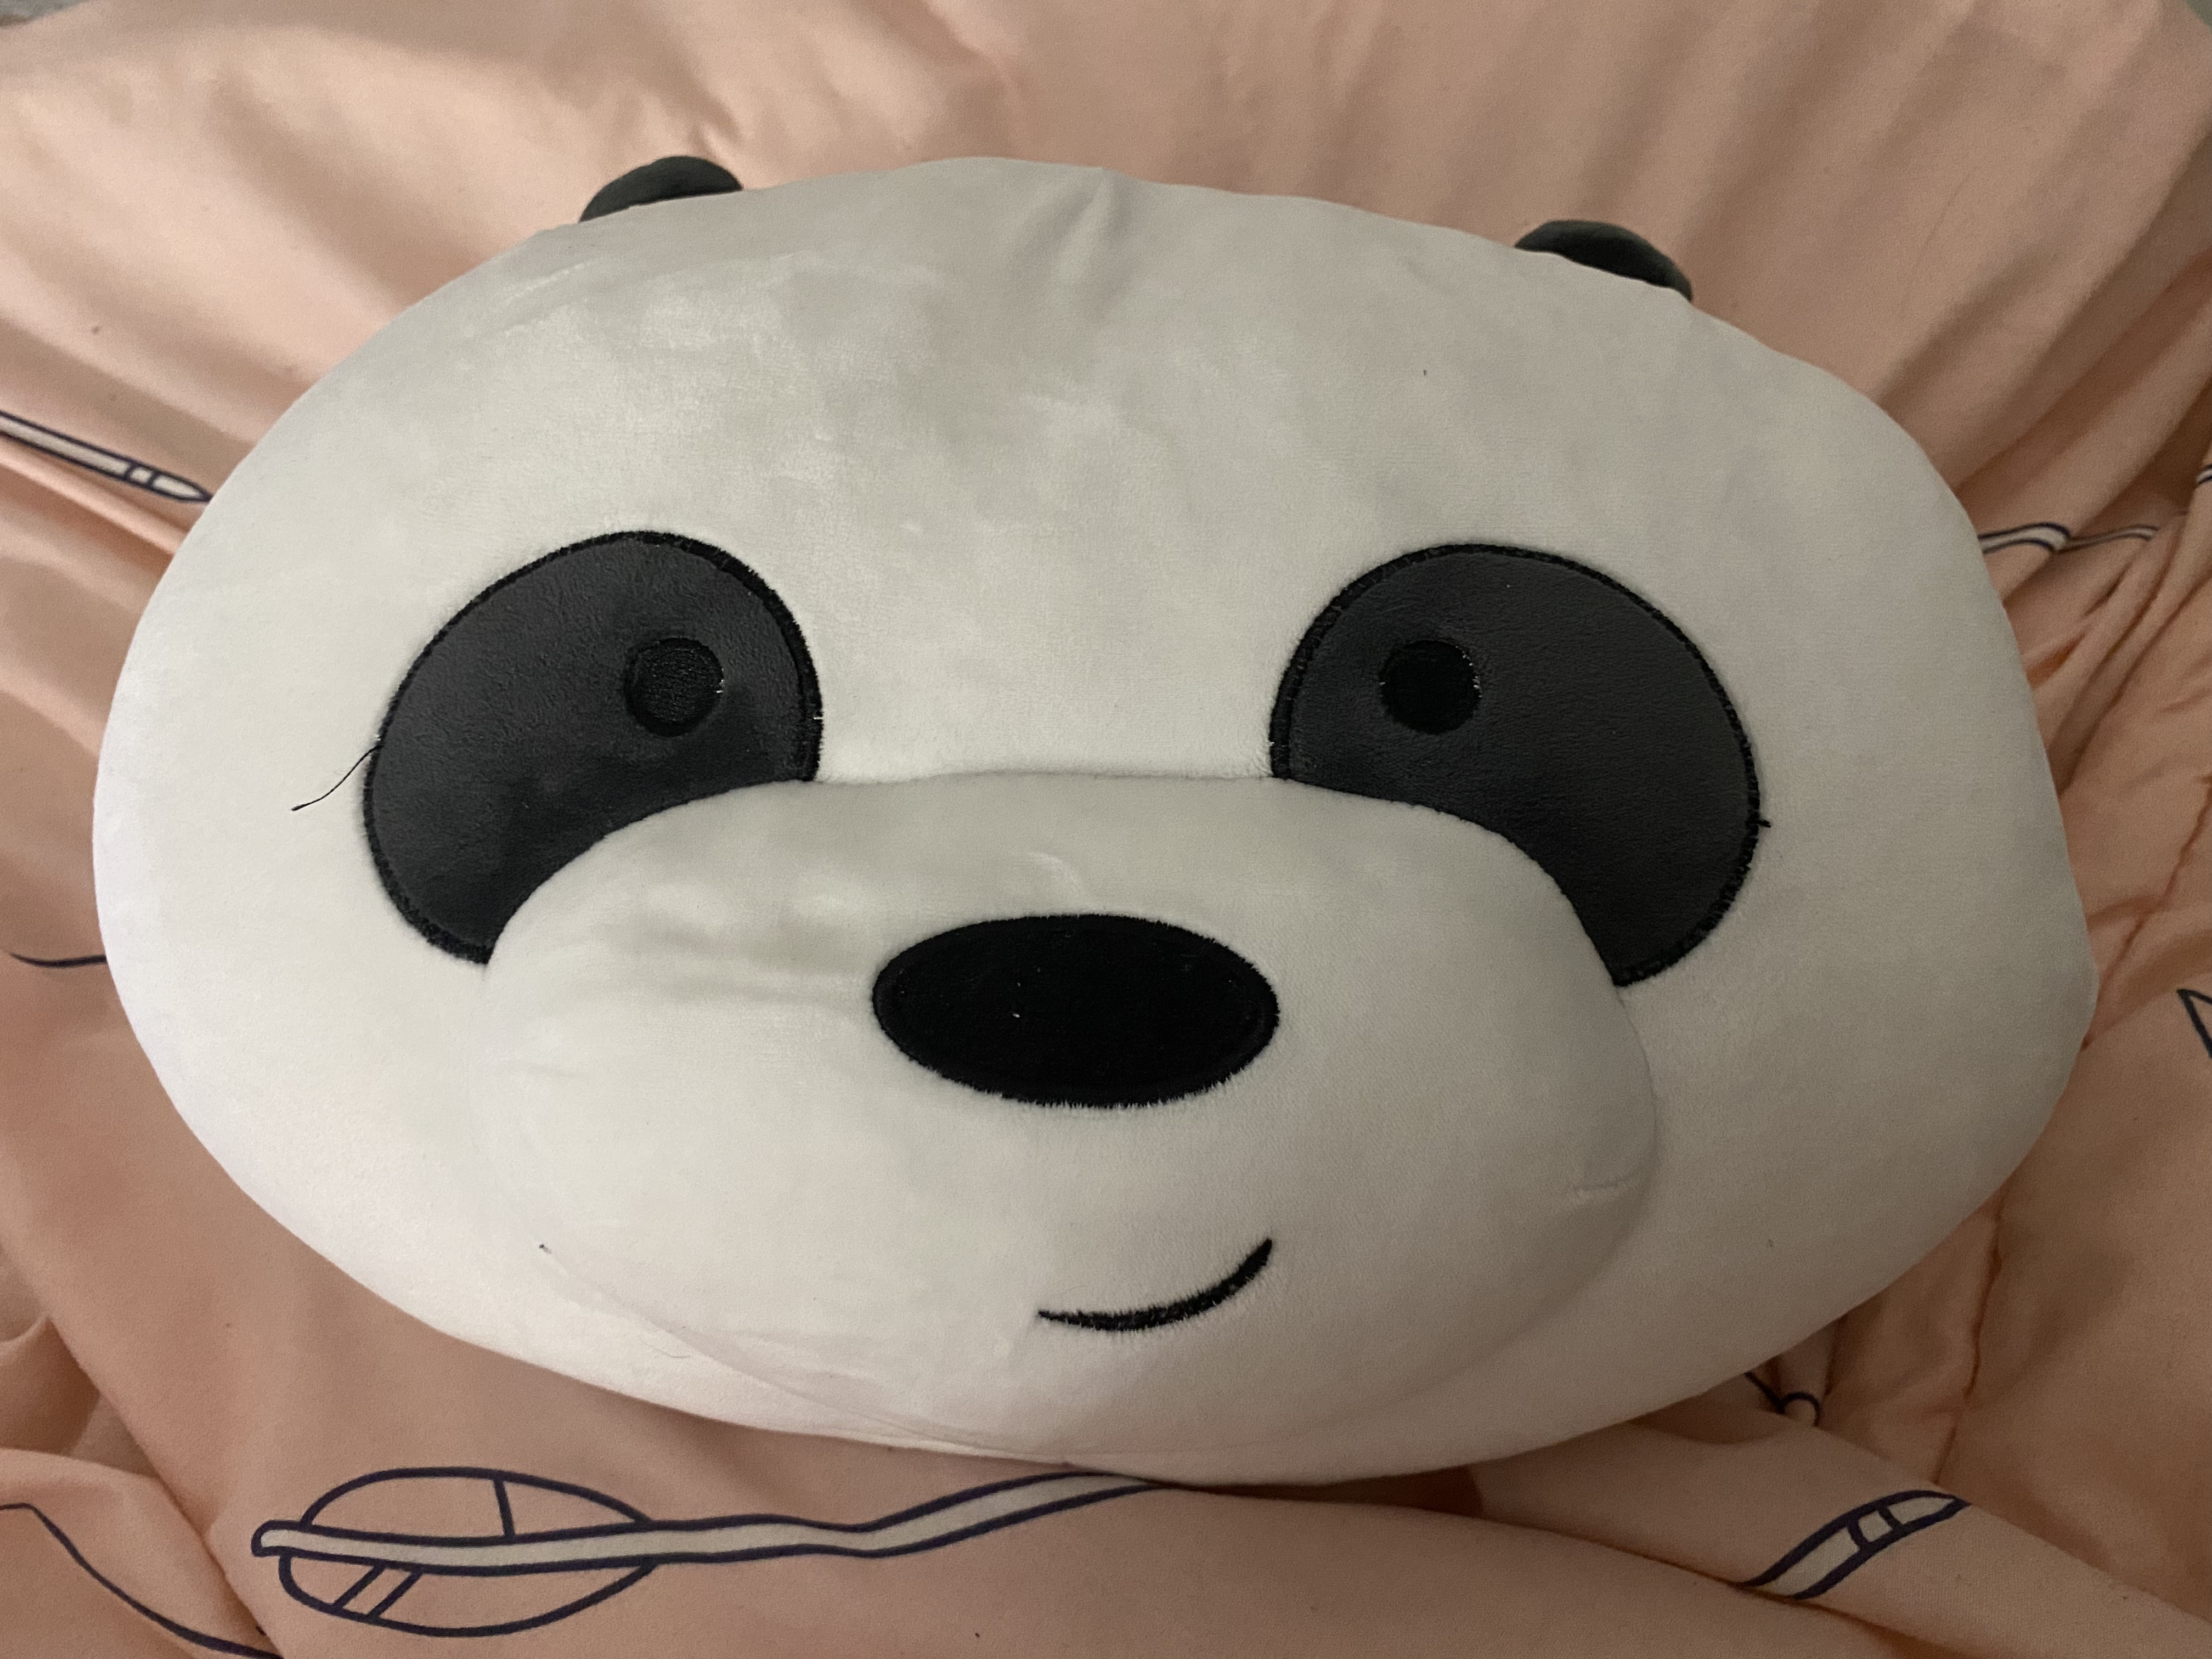
\includegraphics[width=0.8\linewidth]{images/bear.jpg}
\caption{Original image}
\label{fig:bear}
\end{figure}

\begin{lstlisting}[language=Matlab]
% Choose a shade of orange as fill value
orange = [255 127 0]';

% Perform shearing
R = makeresampler({'cubic','nearest'},
                    'fill');
sheared_img = imtransform(img,T,R,
            'FillValues',orange);
h2 = figure; 
imshow(sheared_img);
title('Sheared Image');
\end{lstlisting}

\begin{figure}[h!]
\centering
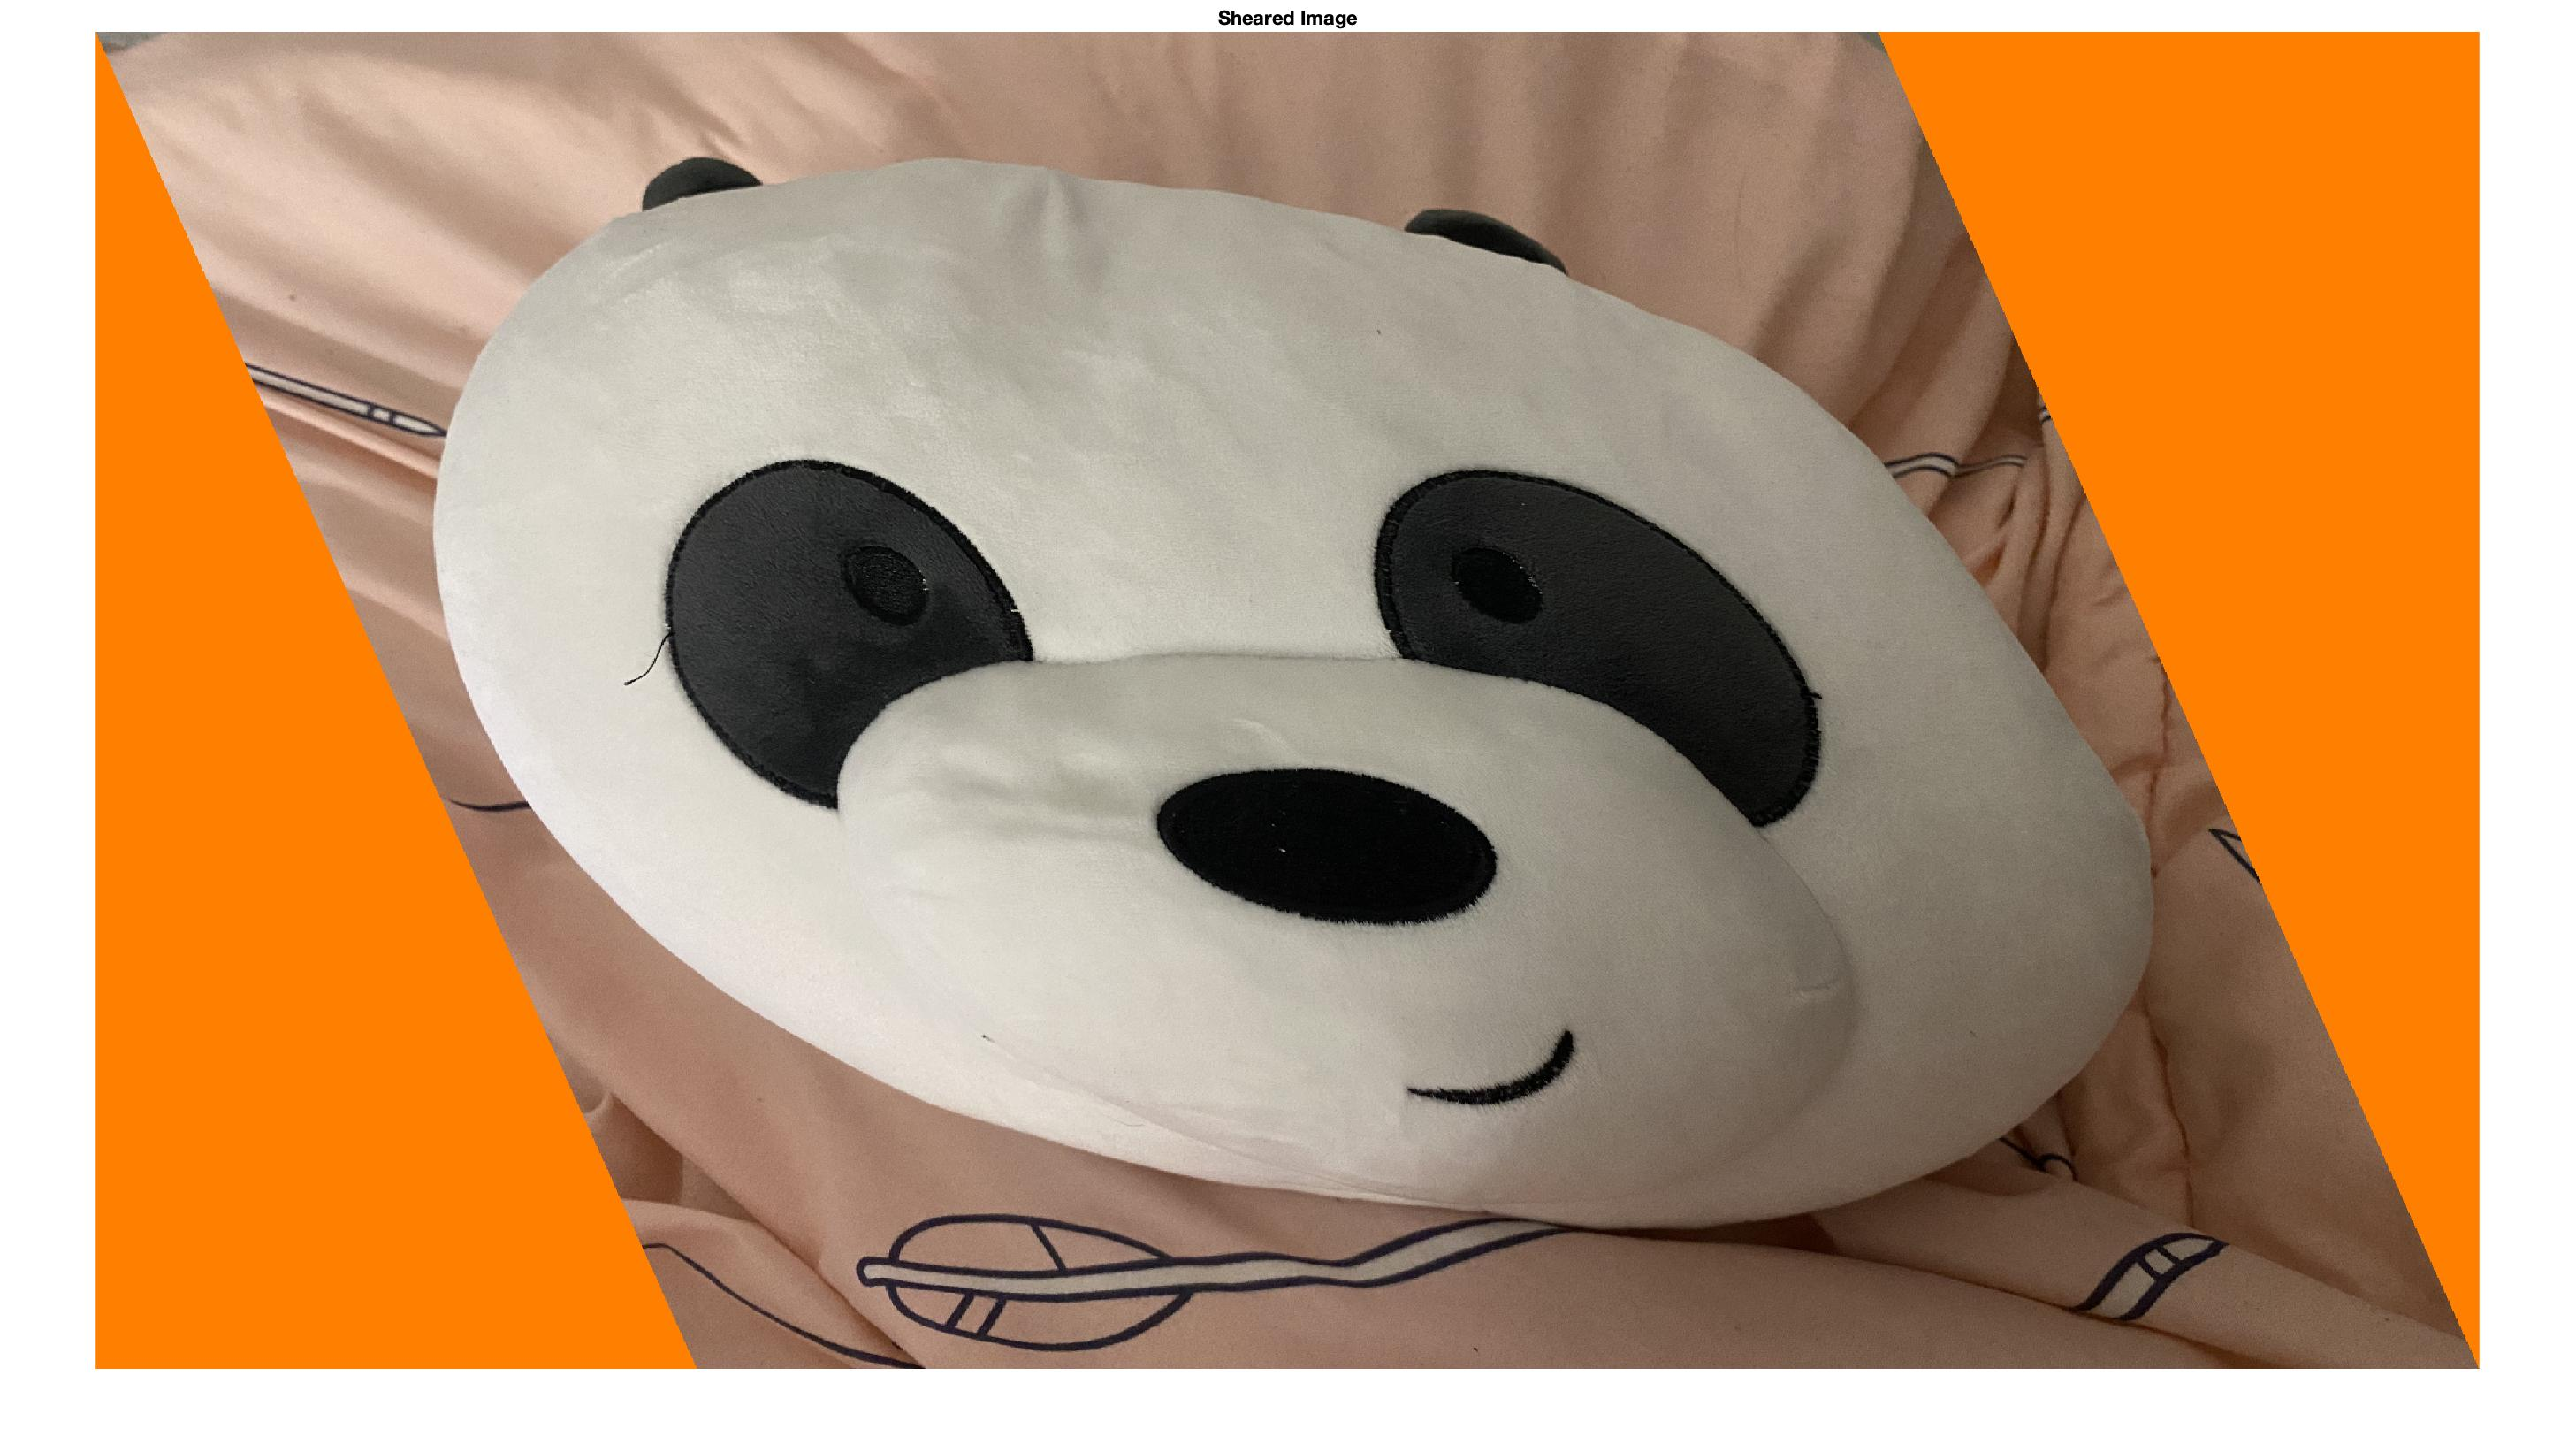
\includegraphics[width=0.8\linewidth]{images/img26.jpg}
\caption{Sheared image}
\label{fig:sheared}
\end{figure}

\subsection{Explore the Transformation}
\begin{lstlisting}[language=Matlab]
% Step 2: Explore the Transformation
[U,V] = meshgrid(0:1008:4032,0:1008:3024);
[X,Y] = tformfwd(T,U,V);
yellow = [1 1 0];

figure(h1);
hold on;
line(U, V, 'Color',yellow);
line(U',V','Color',yellow);

figure(h2);
hold on;
line(X, Y, 'Color',yellow);
line(X',Y','Color',yellow);
\end{lstlisting}

\begin{figure}[h!]
\centering
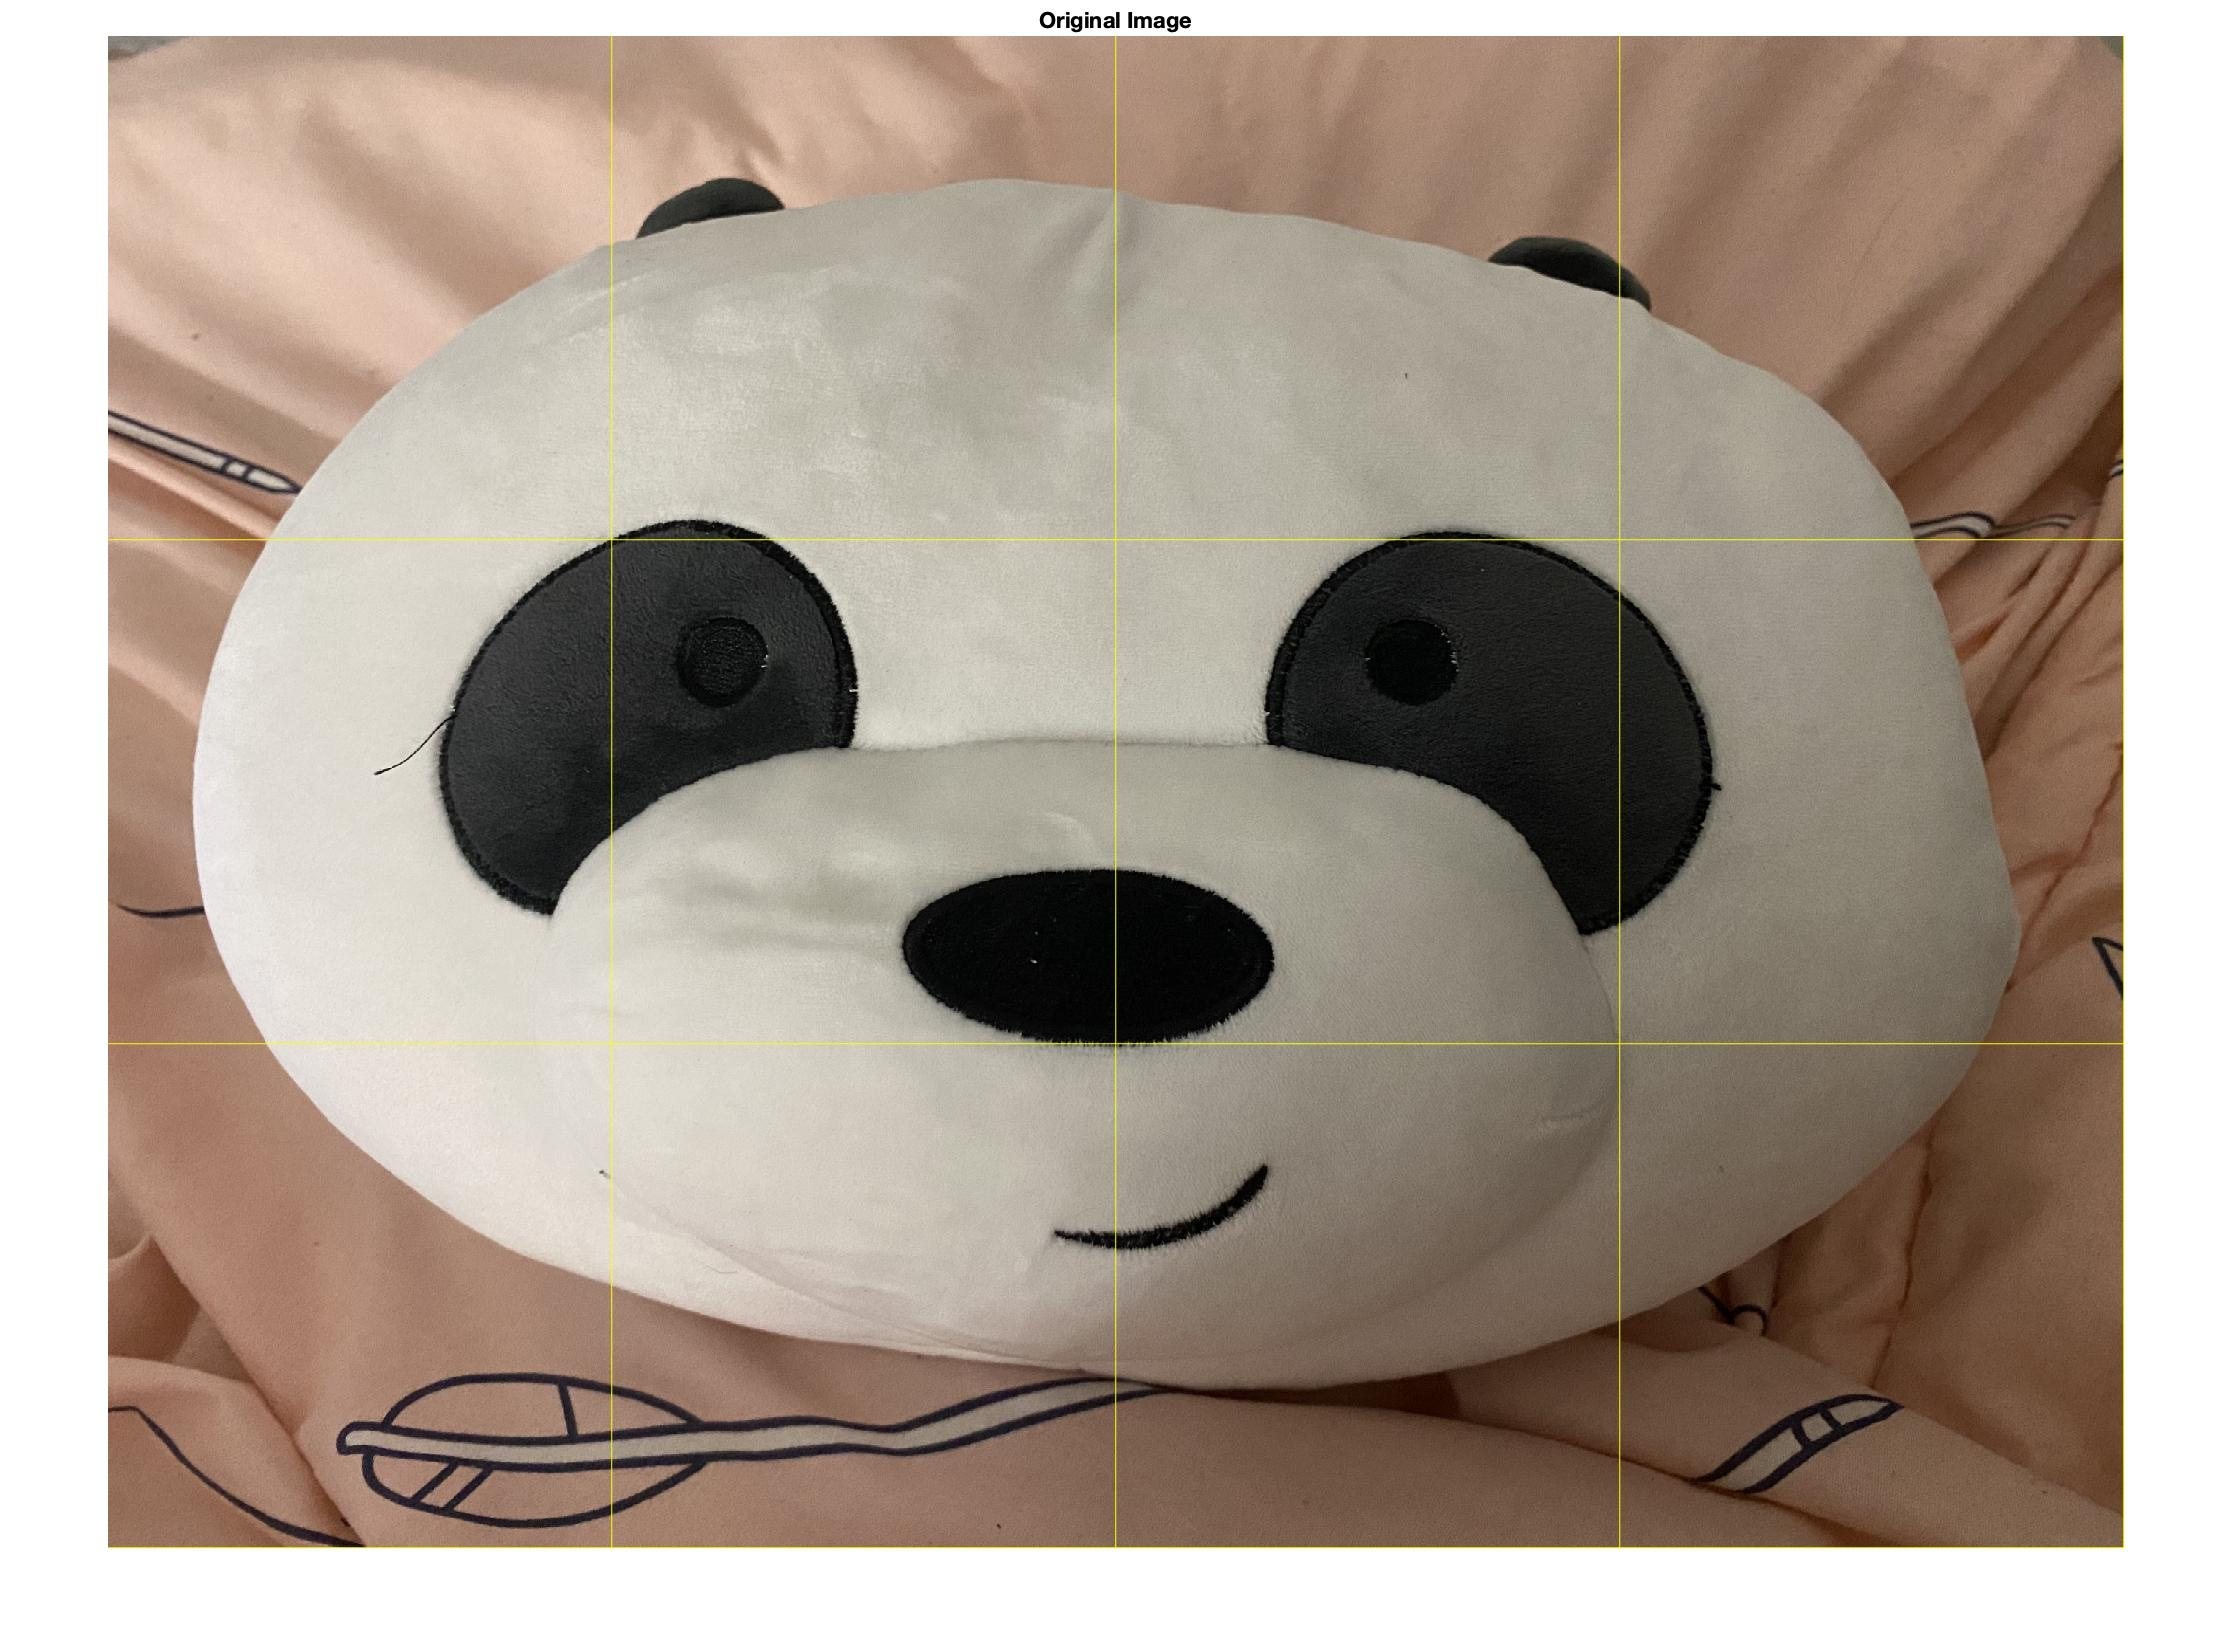
\includegraphics[width=0.8\linewidth]{images/img27.jpg}
\caption{Original image}
\label{fig:oi}
\end{figure}

\begin{figure}[h!]
\centering
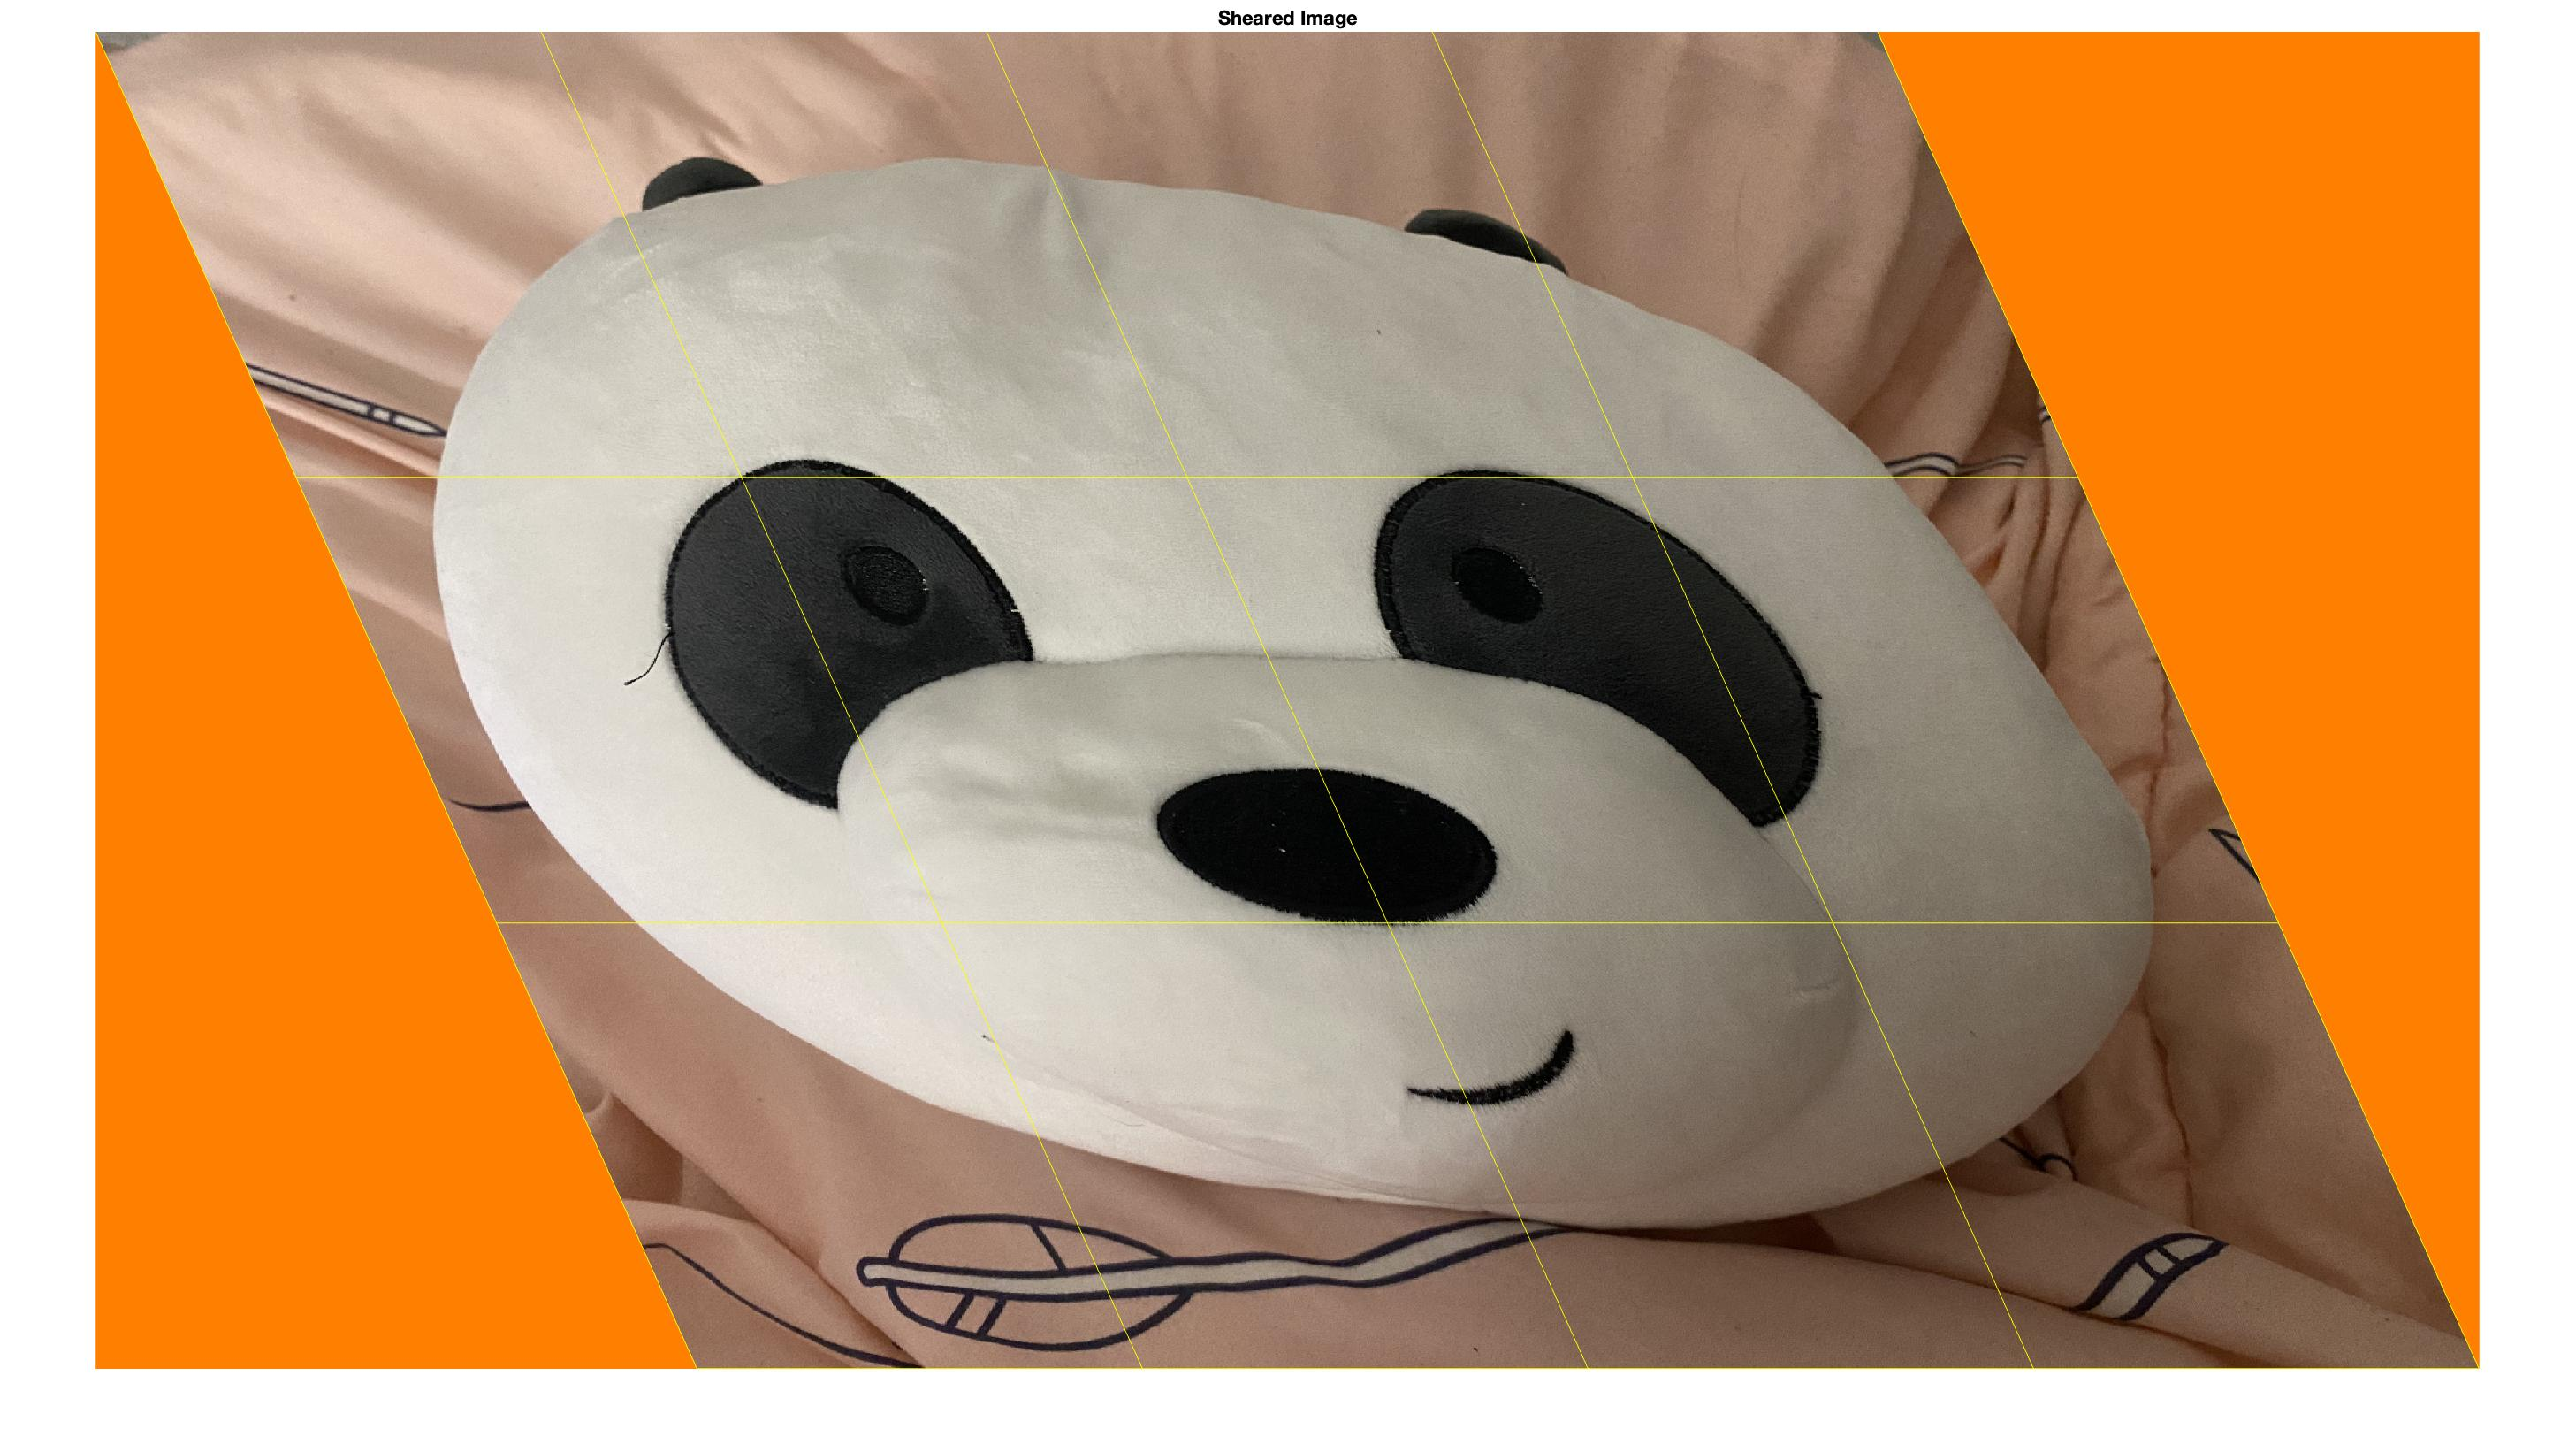
\includegraphics[width=0.8\linewidth]{images/img28.jpg}
\caption{Sheared image}
\label{fig:si}
\end{figure}

\begin{lstlisting}[language=Matlab]
% Do the same thing with 
% an array of circles
for u = 0:1008:4032
    for v = 0:1008:3024
        theta = (0 : 504)' * 
            (2 * pi / 504);
        uc = u + 252*cos(theta);
        vc = v + 252*sin(theta);
        [xc,yc] = tformfwd(T,uc,vc);
        figure(h1); 
        line(uc,vc,'Color',yellow);
        figure(h2); 
        line(xc,yc,'Color',yellow);
    end
end
\end{lstlisting}

\begin{figure}[h!]
\centering
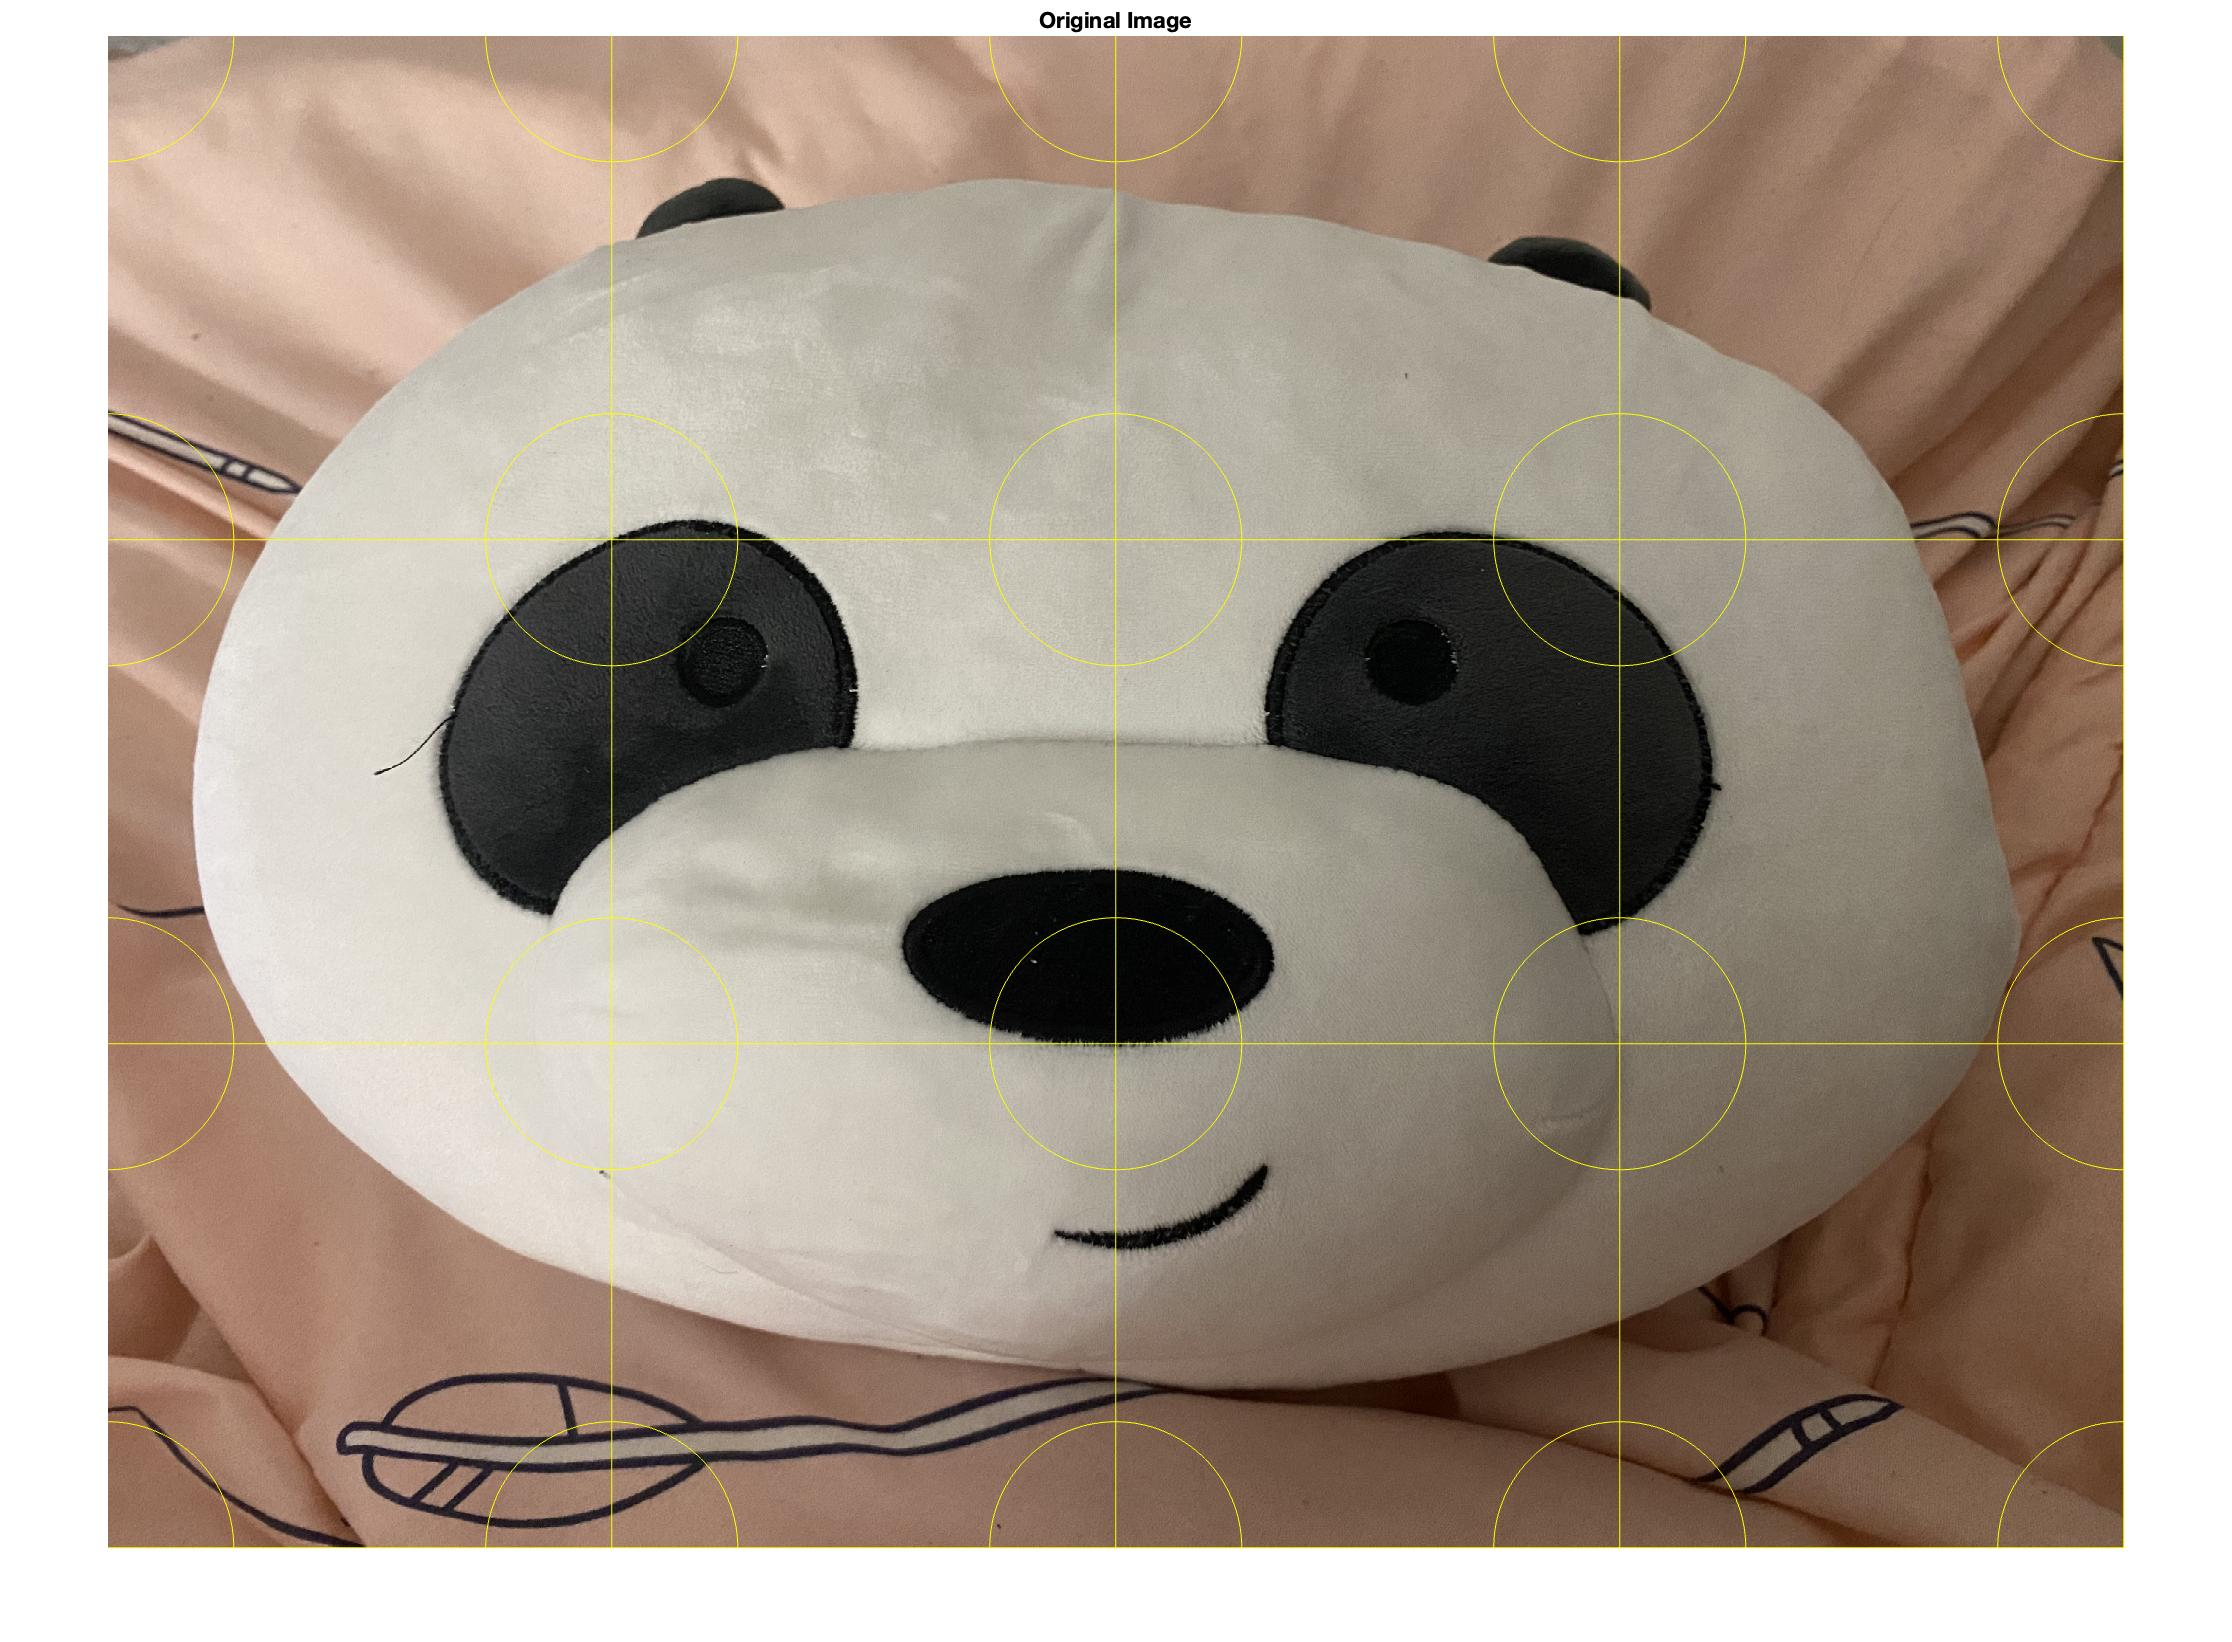
\includegraphics[width=0.8\linewidth]{images/img29.jpg}
\caption{Original image}
\label{fig:abc}
\end{figure}

\begin{figure}[h!]
\centering
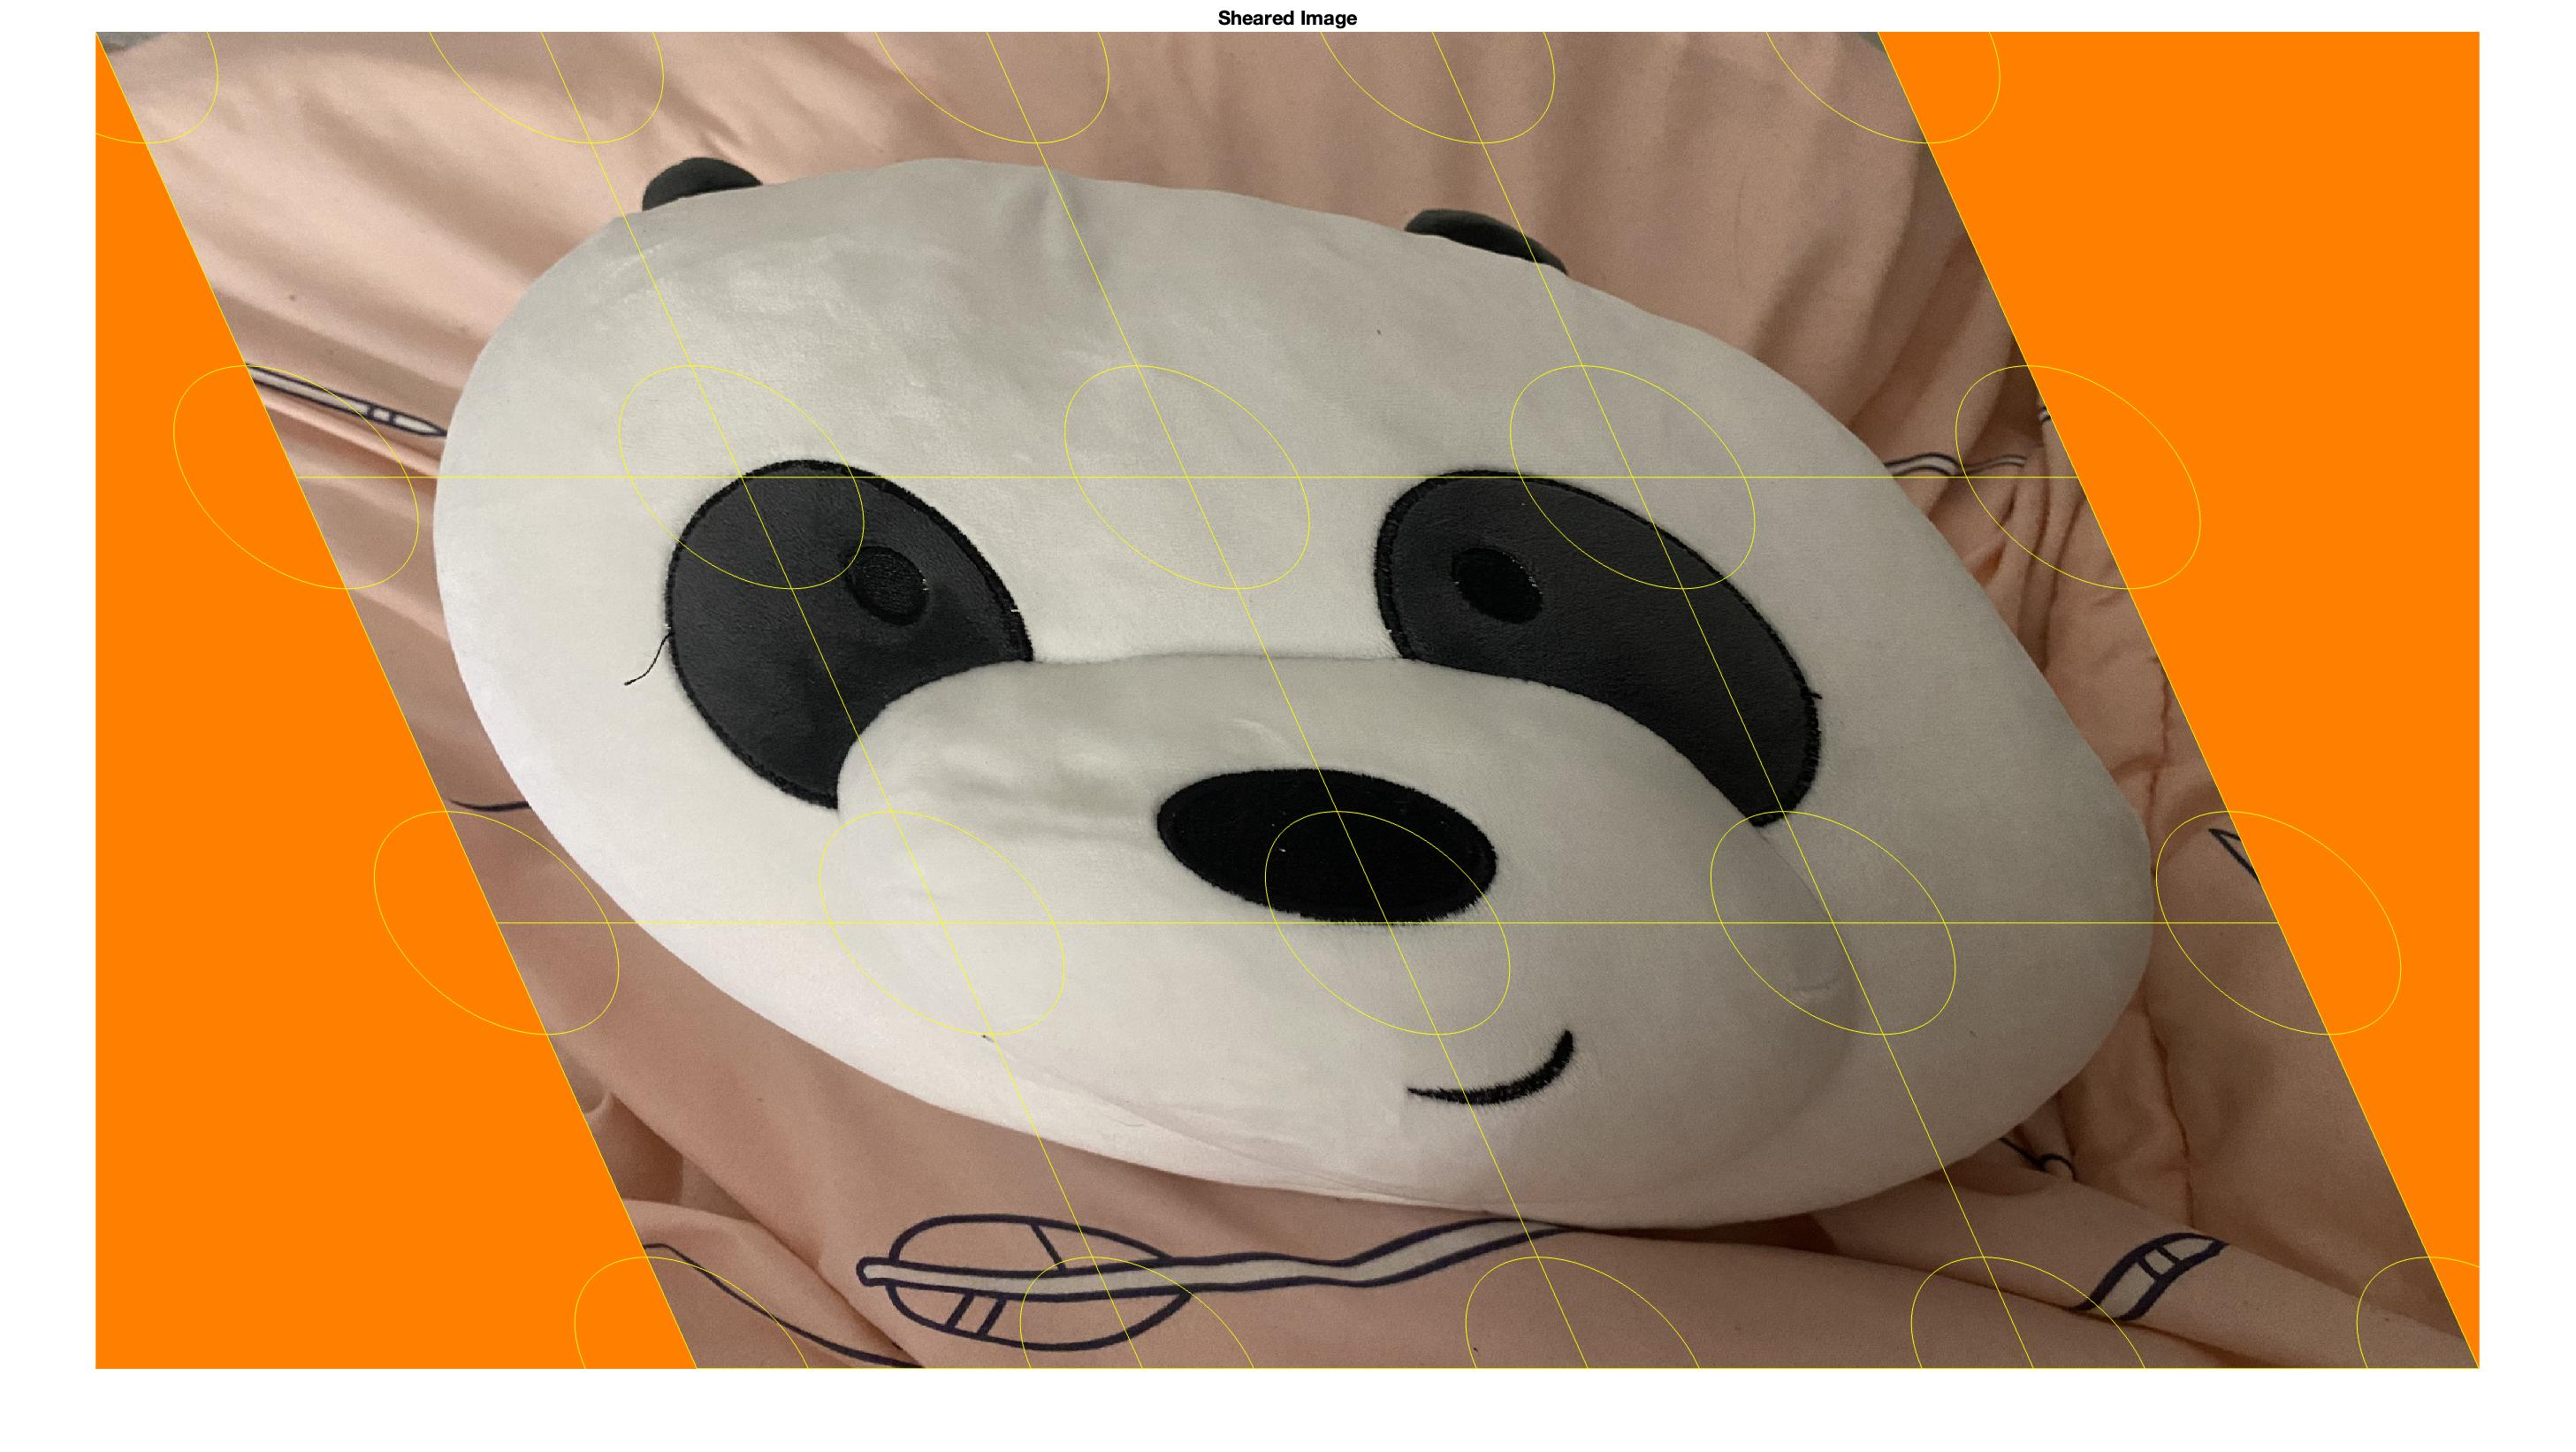
\includegraphics[width=0.8\linewidth]{images/img30.jpg}
\caption{Sheared image}
\label{fig:xyz}
\end{figure}

\subsection{Compare the 'fill', 'replicate', and 'bound' Pad Methods}
\begin{lstlisting}[language=Matlab]
% 'fill' Pad Method
R = makeresampler({'cubic','nearest'},
                'fill');
Bf = imtransform(img,T,R,'XData',[-500 6000],
'YData',[-500 5000],'FillValues',orange);
figure;
imshow(Bf);
title('Pad Method = ''fill''');
% 'replicate' Pad Method
R = makeresampler({'cubic','nearest'},
                'replicate');
Br = imtransform(img,T,R,'XData',
[-500 6000],'YData', [-500 5000]);
figure;
imshow(Br);
title('Pad Method = ''replicate''');
% 'bound' Pad Method
R = makeresampler({'cubic','nearest'}, 
                'bound');
Bb = imtransform(img,T,R,'XData',[-500 6000],
'YData',[-500 5000],'FillValues',orange);
figure;
imshow(Bb);
title('Pad Method = ''bound''');
\end{lstlisting}

\begin{figure}[h!]
\centering
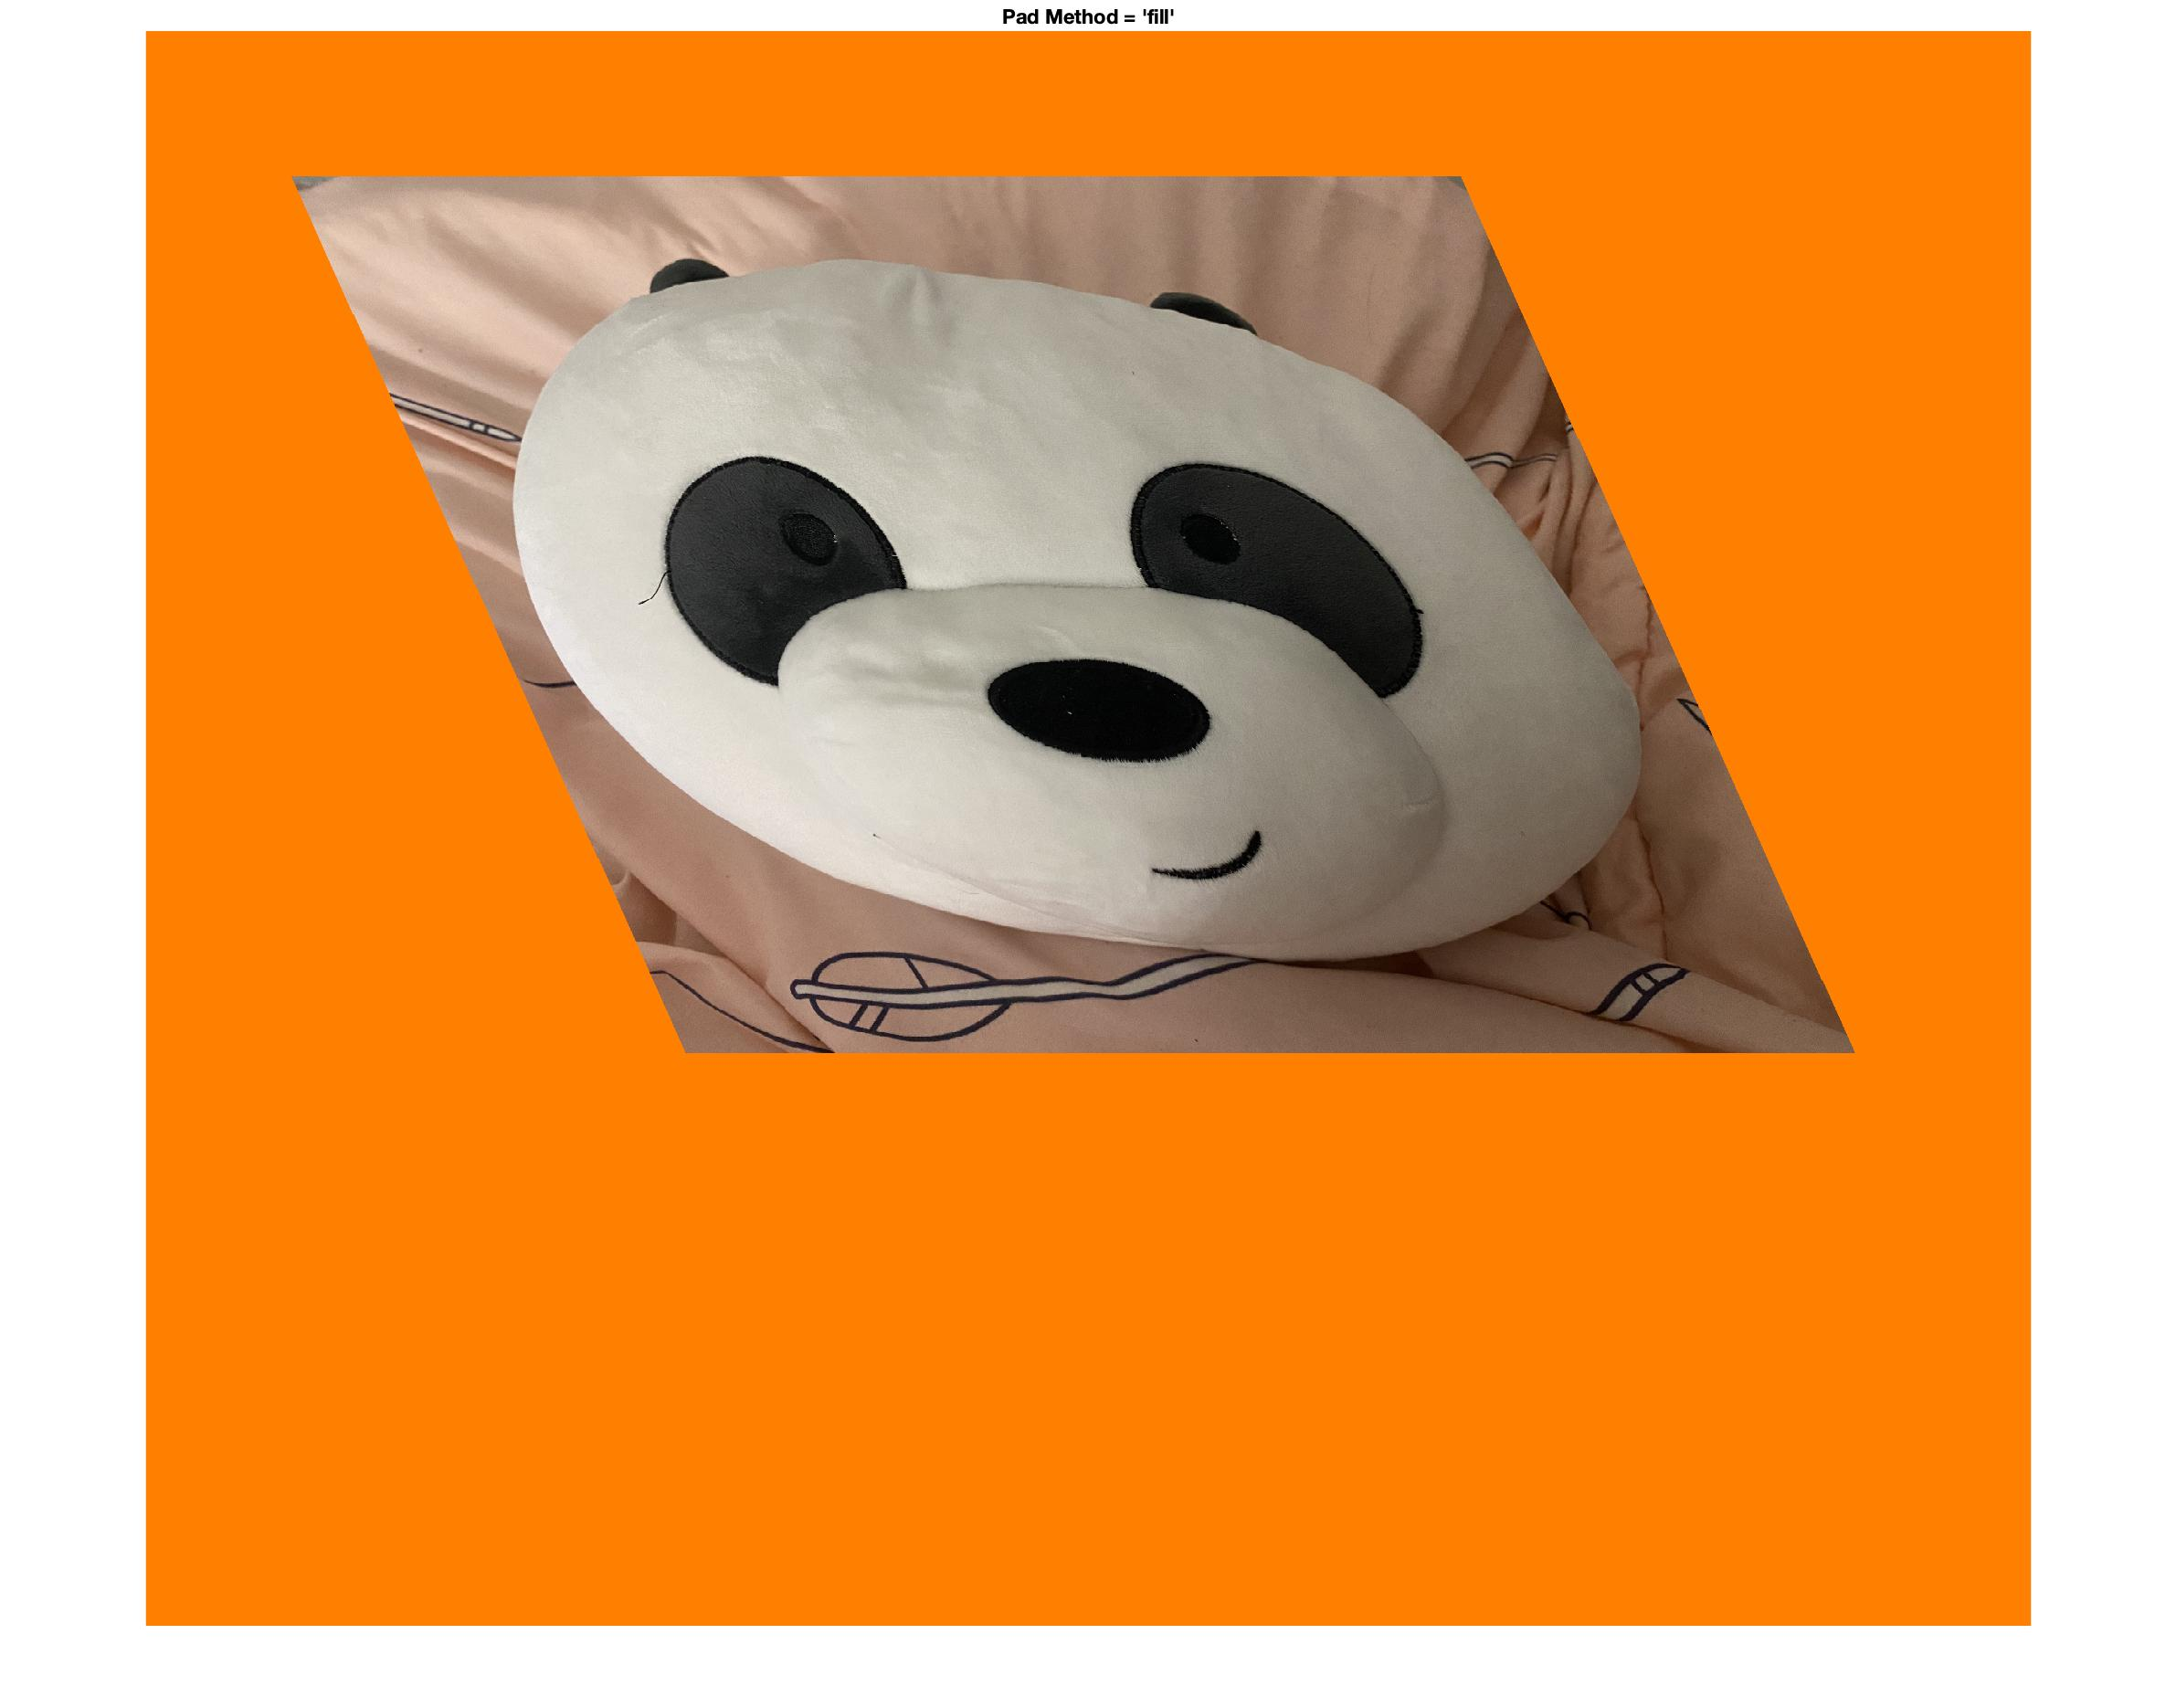
\includegraphics[width=0.7\linewidth]{images/img31.jpg}
\caption{Pad Method = ''fill''}
\label{fig:fill}
\end{figure}

\begin{figure}[h!]
\centering
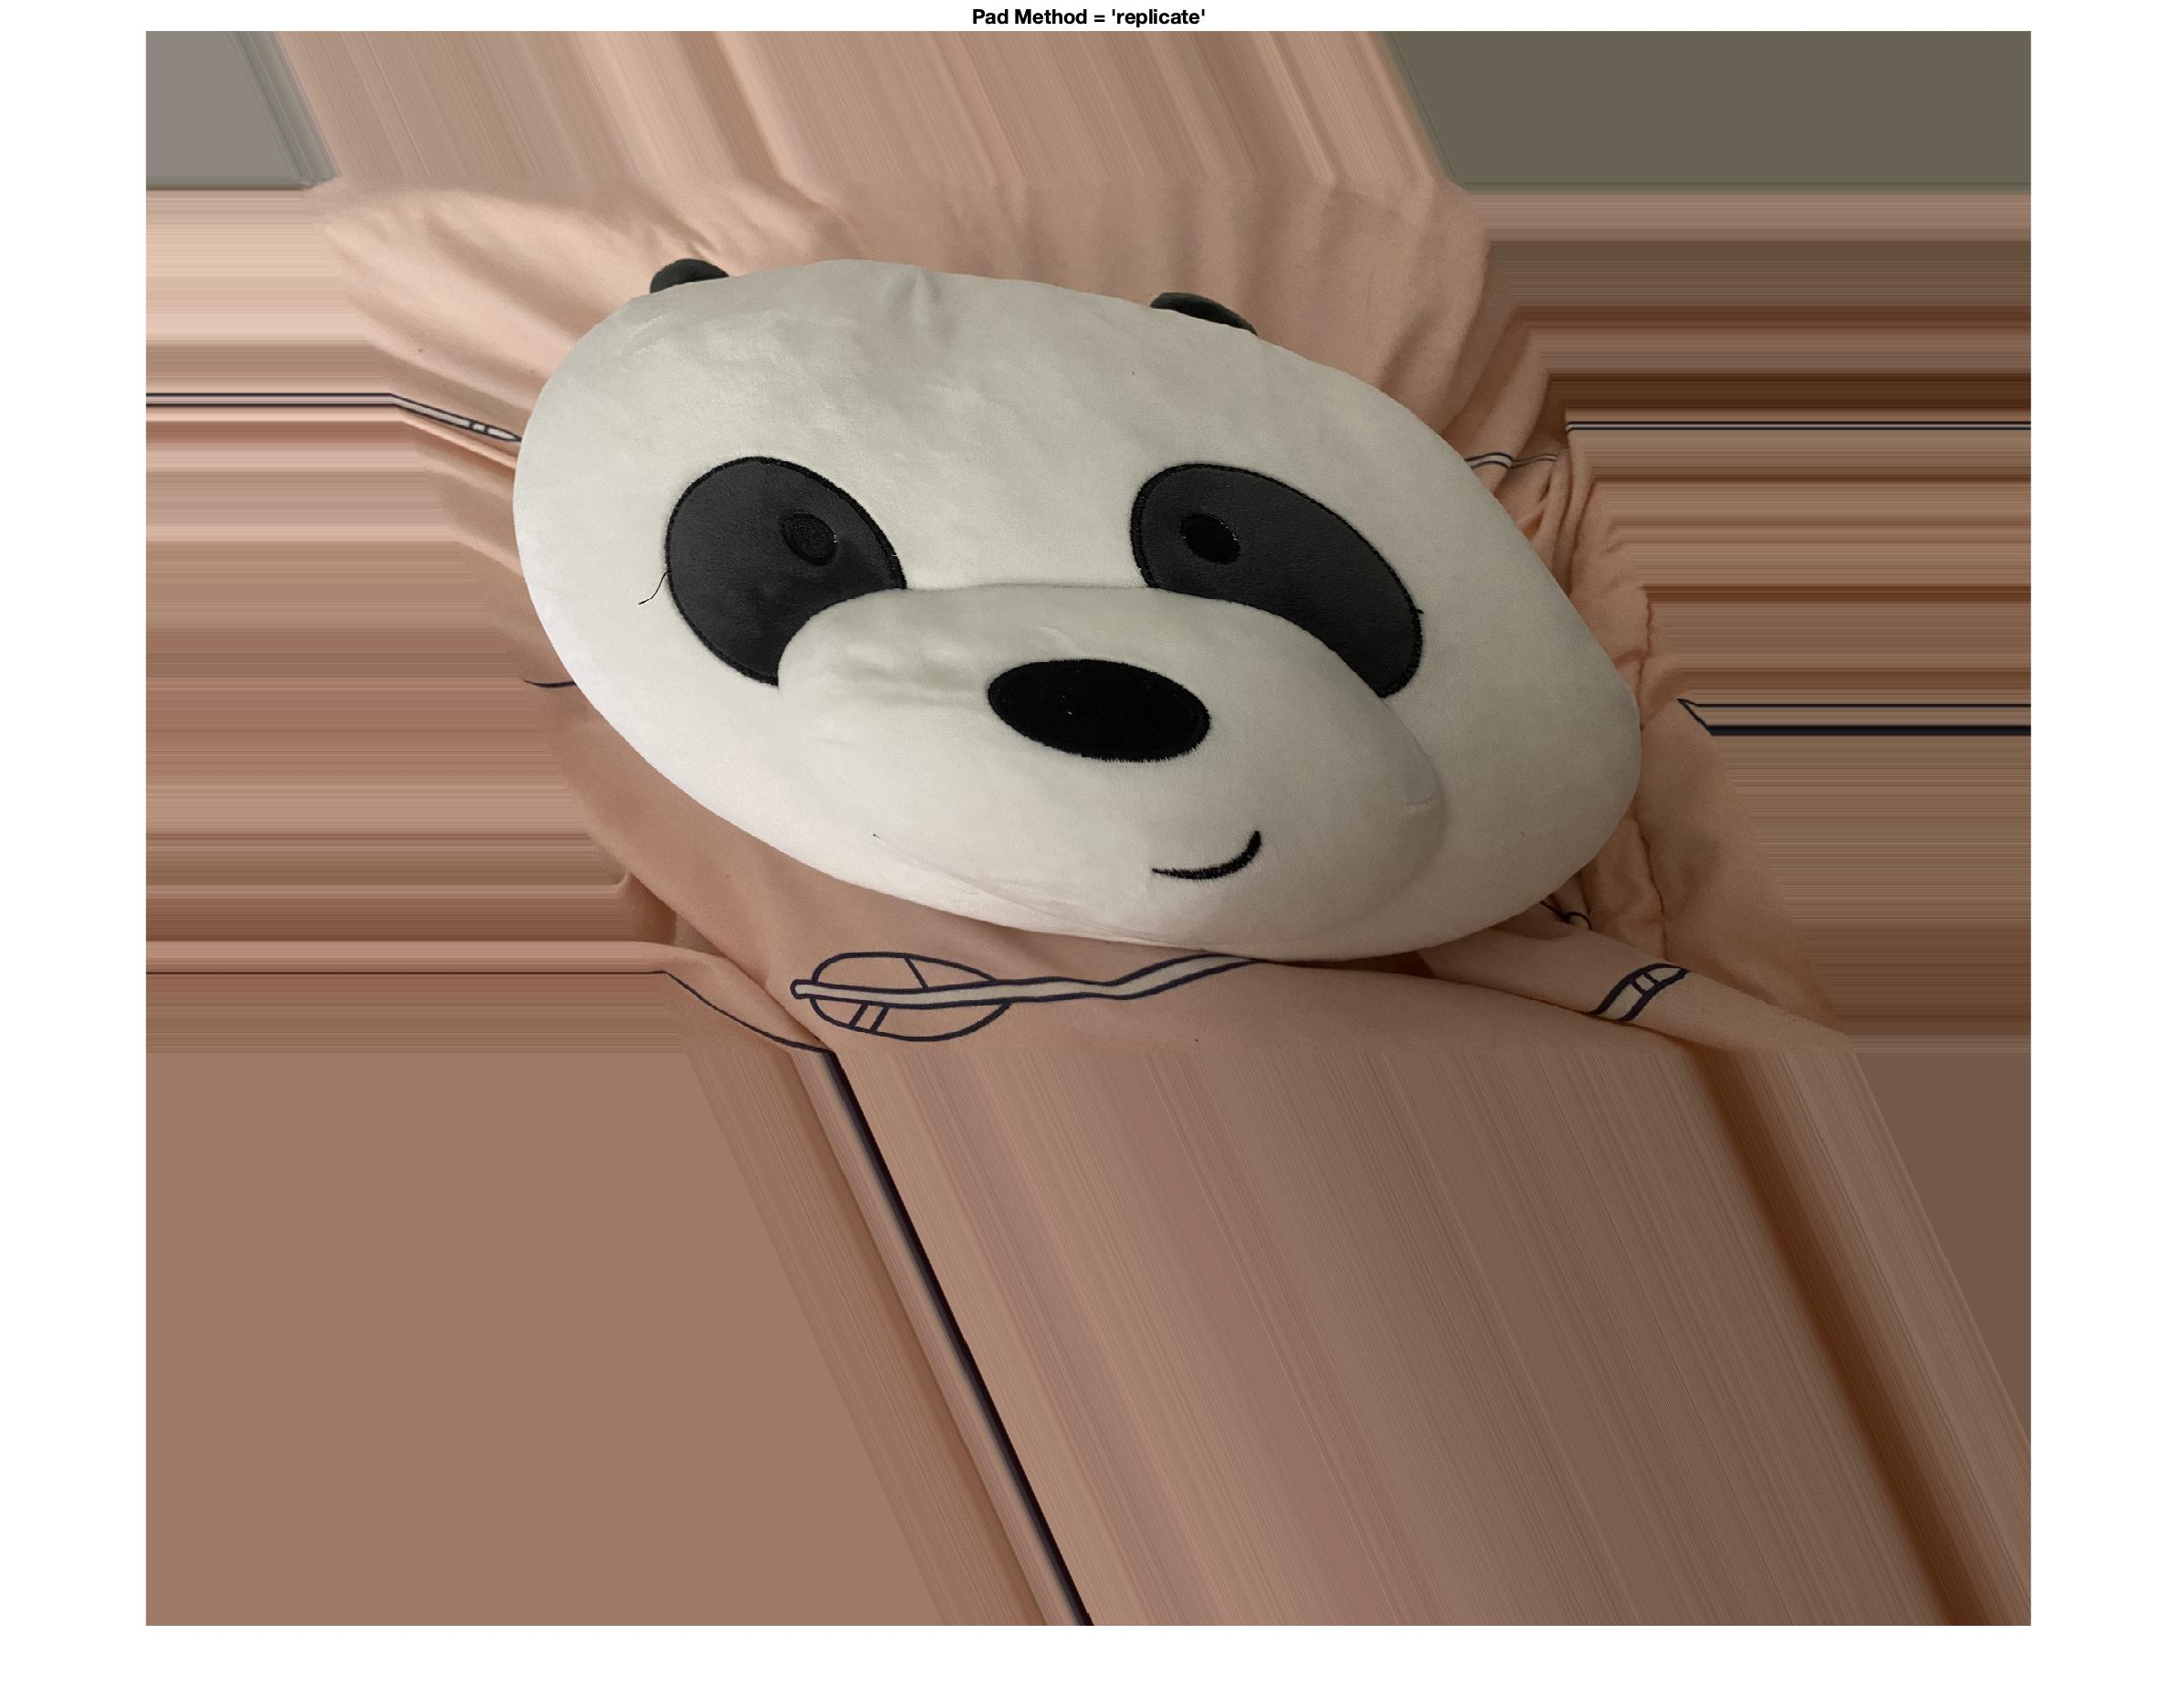
\includegraphics[width=0.7\linewidth]{images/img32.jpg}
\caption{Pad Method = ''replicate''}
\label{fig:replicate}
\end{figure}

\begin{figure}[h!]
\centering
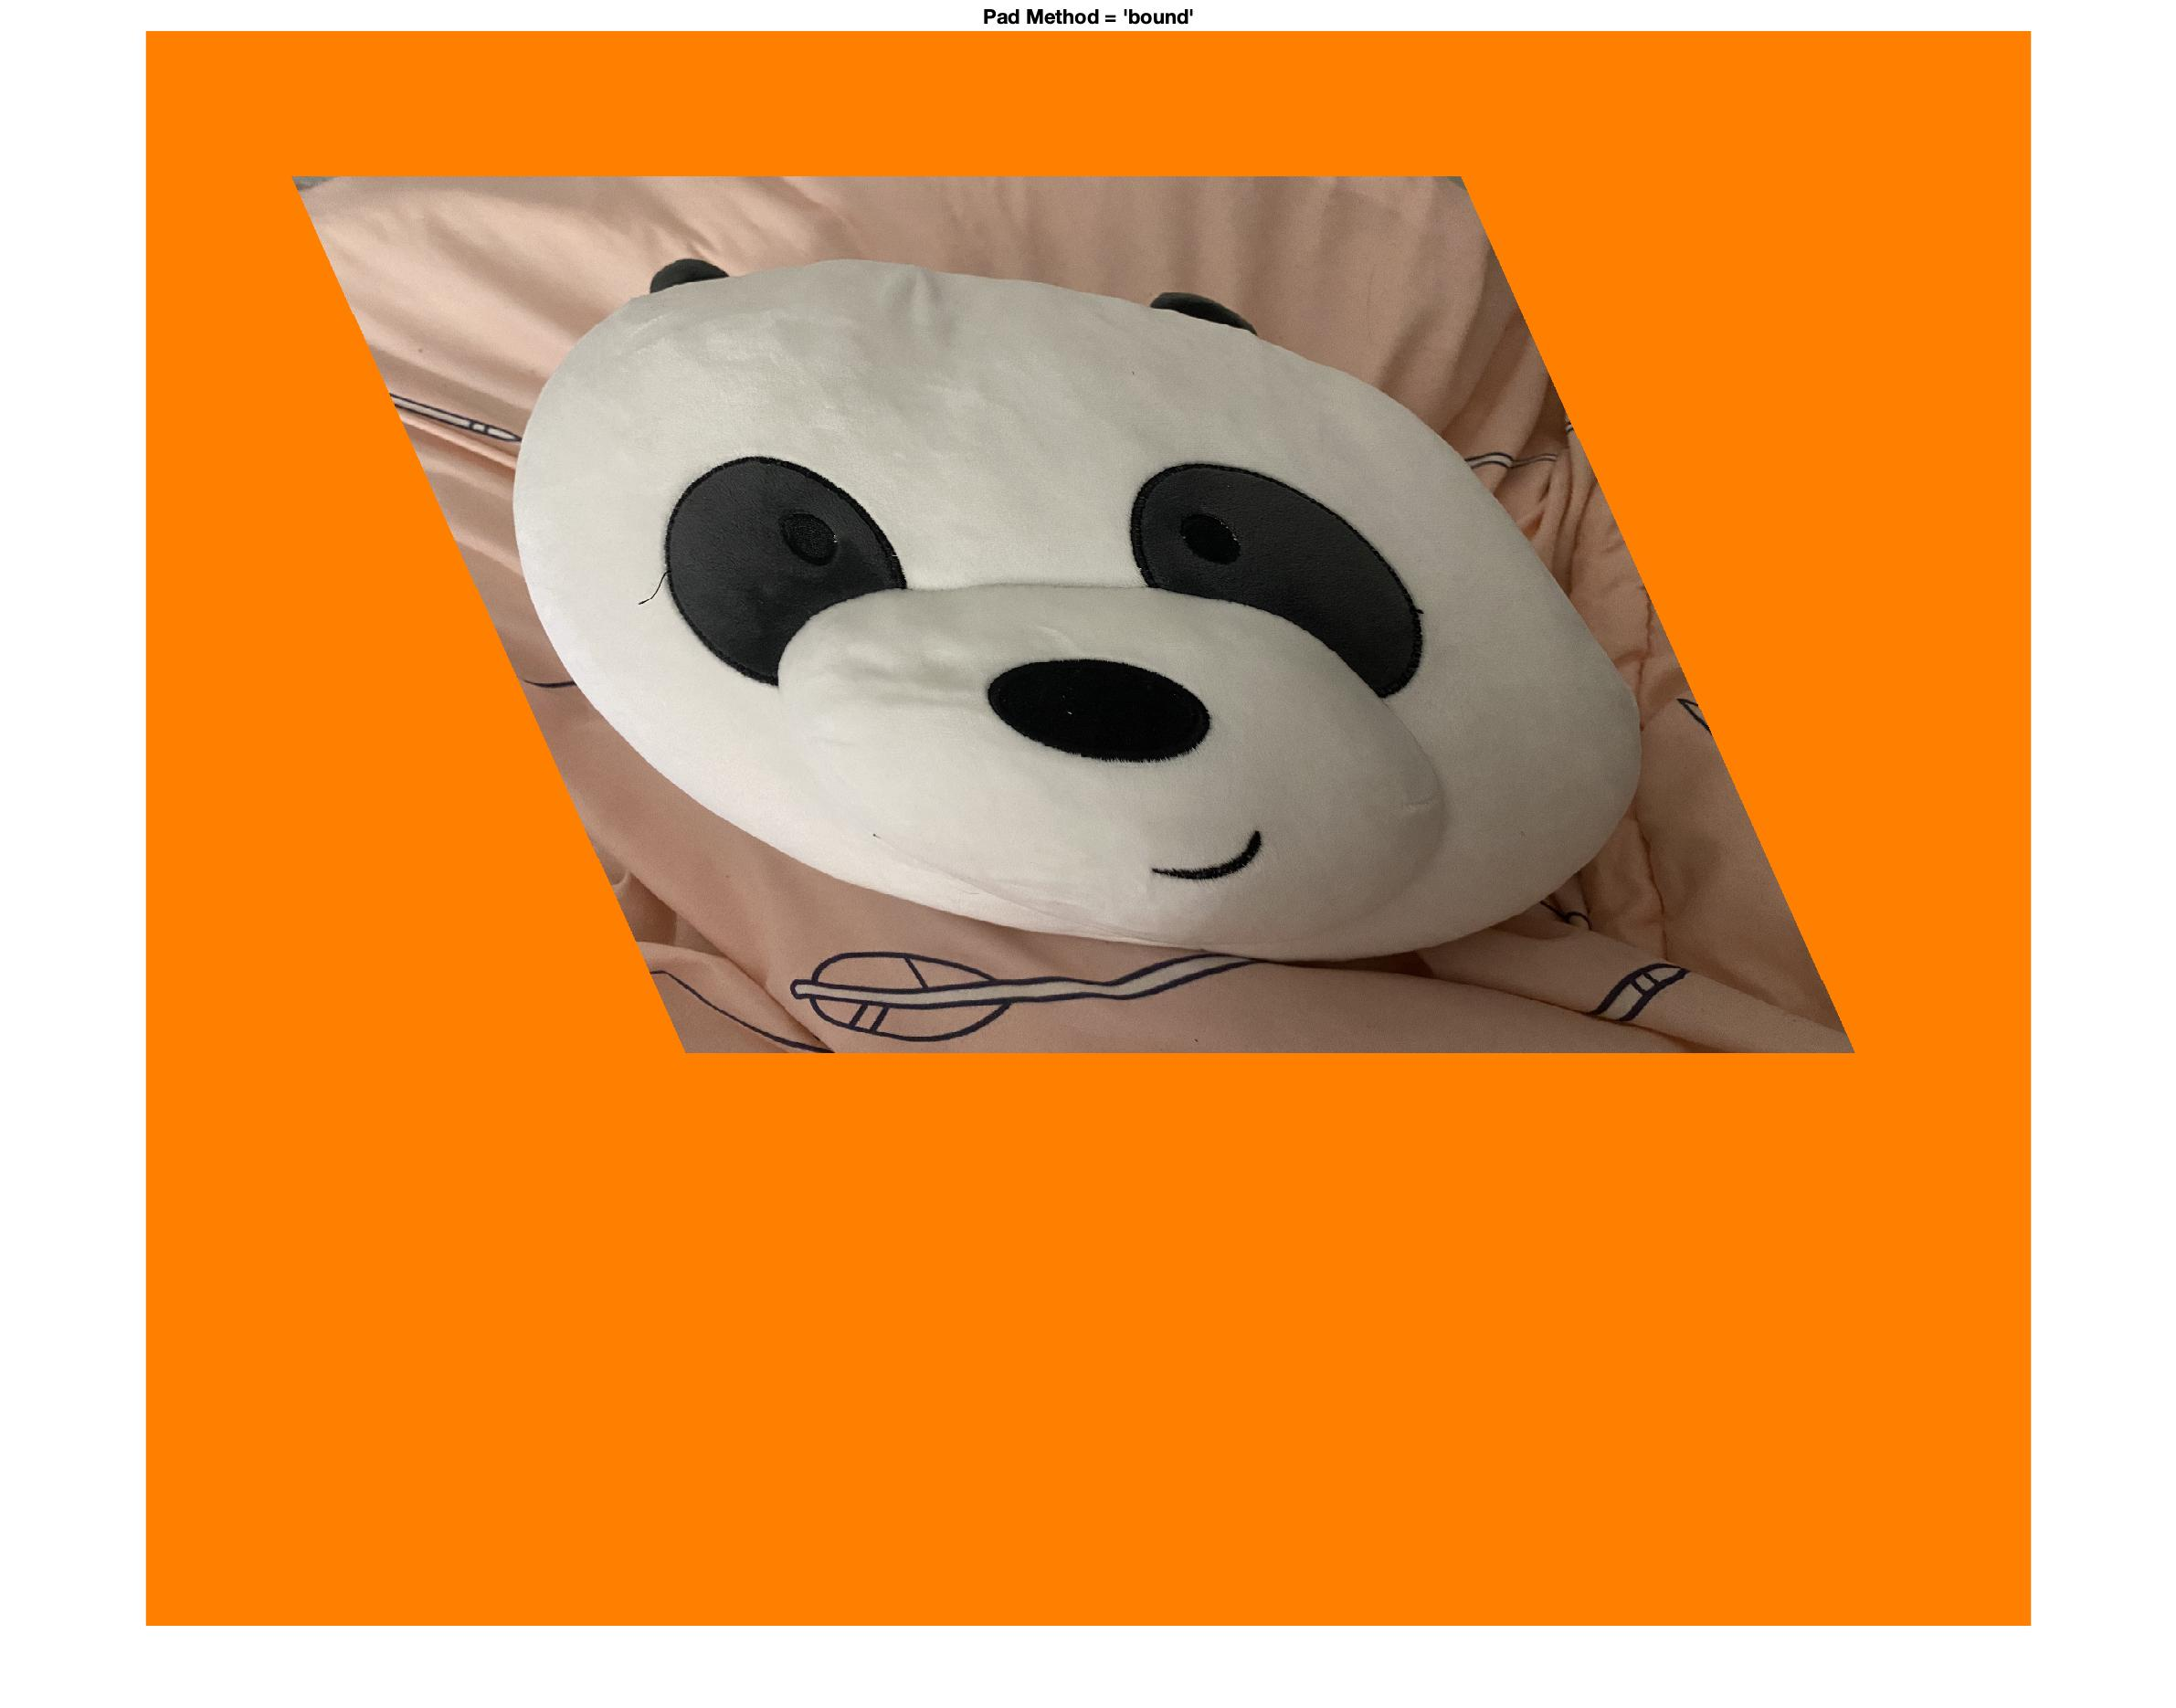
\includegraphics[width=0.7\linewidth]{images/img33.jpg}
\caption{Pad Method = ''bound''}
\label{fig:bound}
\end{figure}

\clearpage

\begin{lstlisting}[language=Matlab]
% Compare 'fill' and 'bound' Pad Method
R = makeresampler({'cubic','nearest'},
                    'fill');
Cf=imtransform(img,T,R,'XData',[5383 5399],
'YData',[3014 3029],'FillValues',orange);

R = makeresampler({'cubic','nearest'},
                    'bound');
Cb=imtransform(img,T,R,'XData',[5383 5399],
'YData',[3014 3029],'FillValues',orange);

Cf = imresize(Cf,12,'nearest');
Cb = imresize(Cb,12,'nearest');

figure;
imshow(Cf); 
title('Pad Method = ''fill''');

figure;
imshow(Cb); 
title('Pad Method = ''bound''');
\end{lstlisting}

\begin{figure}[h!]
\centering
\begin{subfigure}[b]{0.7\linewidth}
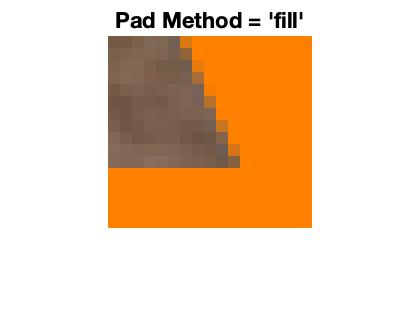
\includegraphics[width=\linewidth]{images/img34.jpg}
\end{subfigure}
\begin{subfigure}[b]{0.7\linewidth}
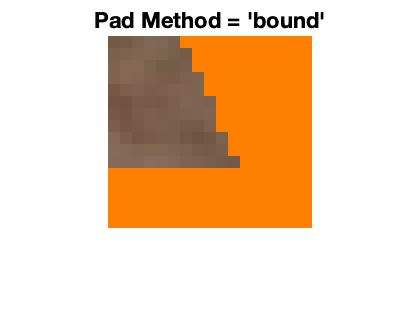
\includegraphics[width=\linewidth]{images/img35.jpg}
\end{subfigure}
\caption{Compare 'fill' and 'bound' Pad Method}
\label{fig: compare}
\end{figure}

\subsection{Exercise the 'circular' and 'symmetric' Pad Methods}
\begin{lstlisting}[language=Matlab]
% 'circular' Pad Method
Thalf = maketform('affine',[1 0; a 1; 0 0]/2);

R = makeresampler({'cubic','nearest'},'circular');
Bc = imtransform(img,Thalf,R,'XData',[-500 6000],
'YData',[-500 5000],'FillValues',orange);
figure;
imshow(Bc);
title('Pad Method = ''circular''');

% 'symmetric' Pad Method
R = makeresampler({'cubic','nearest'},'symmetric');
Bs = imtransform(img,Thalf,R,'XData',[-500 6000],
'YData',[-500 5000],'FillValues',orange);
figure;
imshow(Bs);
title('Pad Method = ''symmetric''');
\end{lstlisting}

\begin{figure}[h!]
\centering
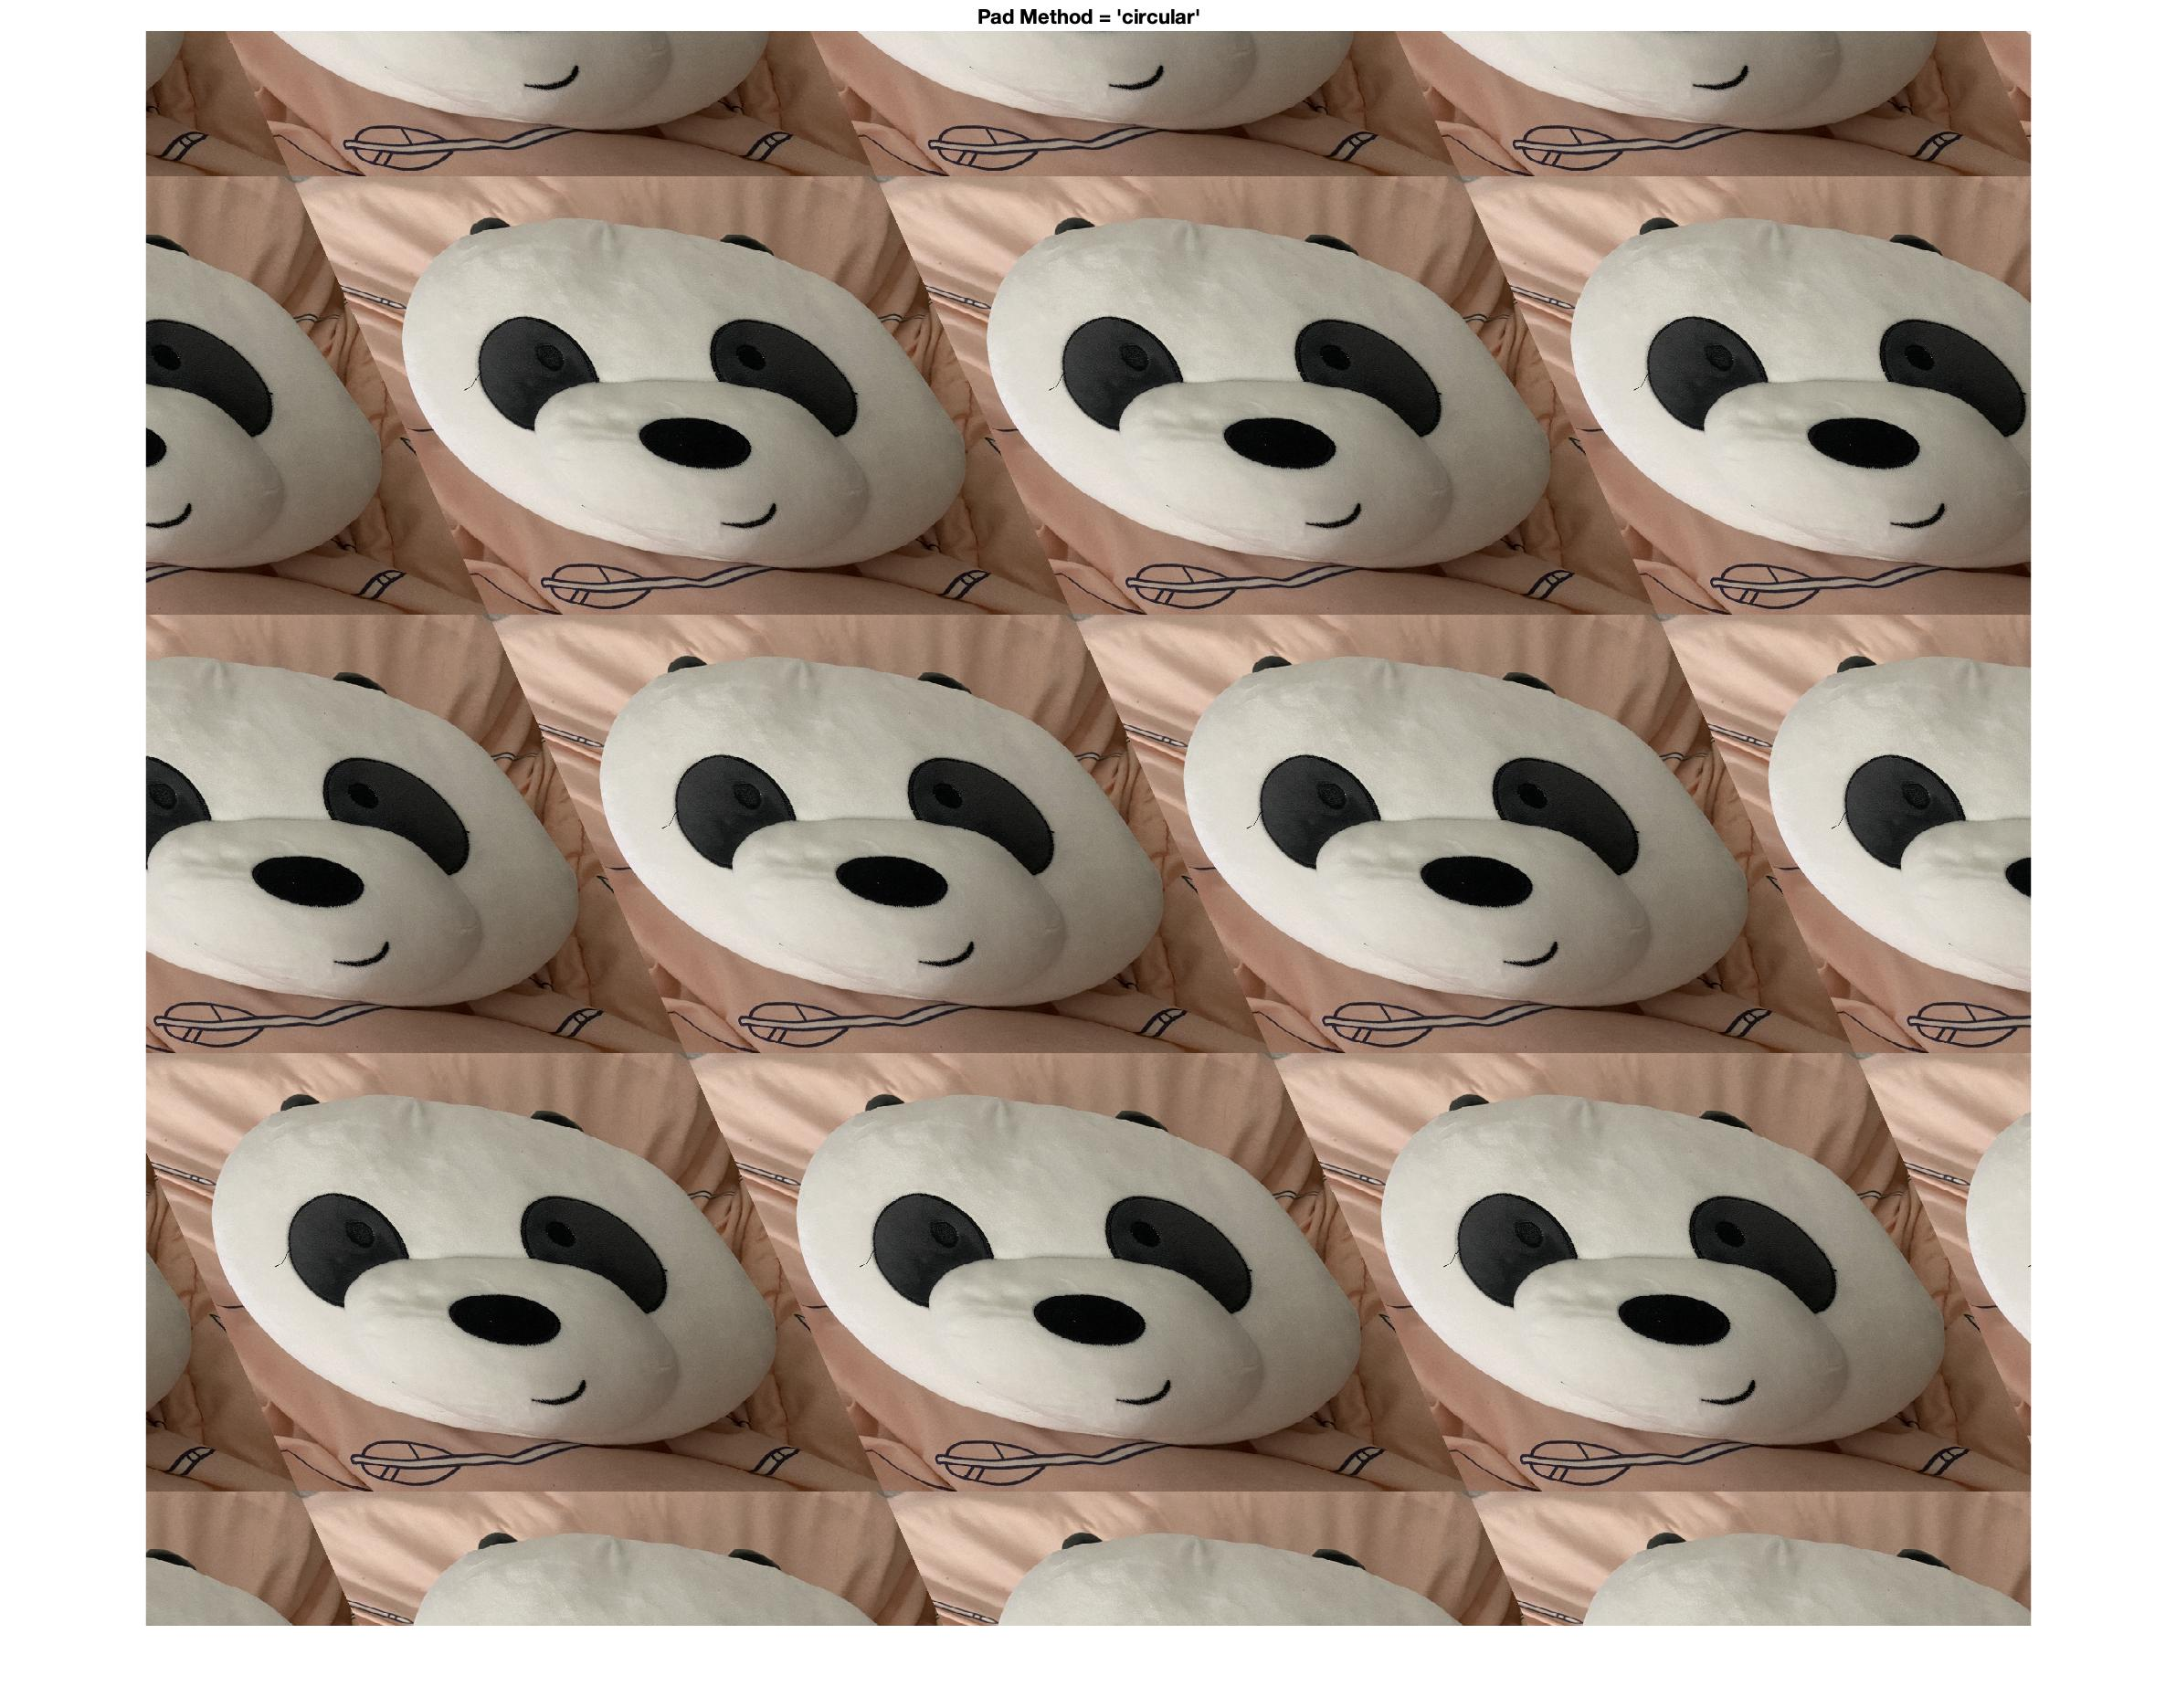
\includegraphics[width=0.8\linewidth]{images/img36.jpg}
\caption{Pad Method = ''circular''}
\label{fig:circular}
\end{figure}

\begin{figure}[h!]
\centering
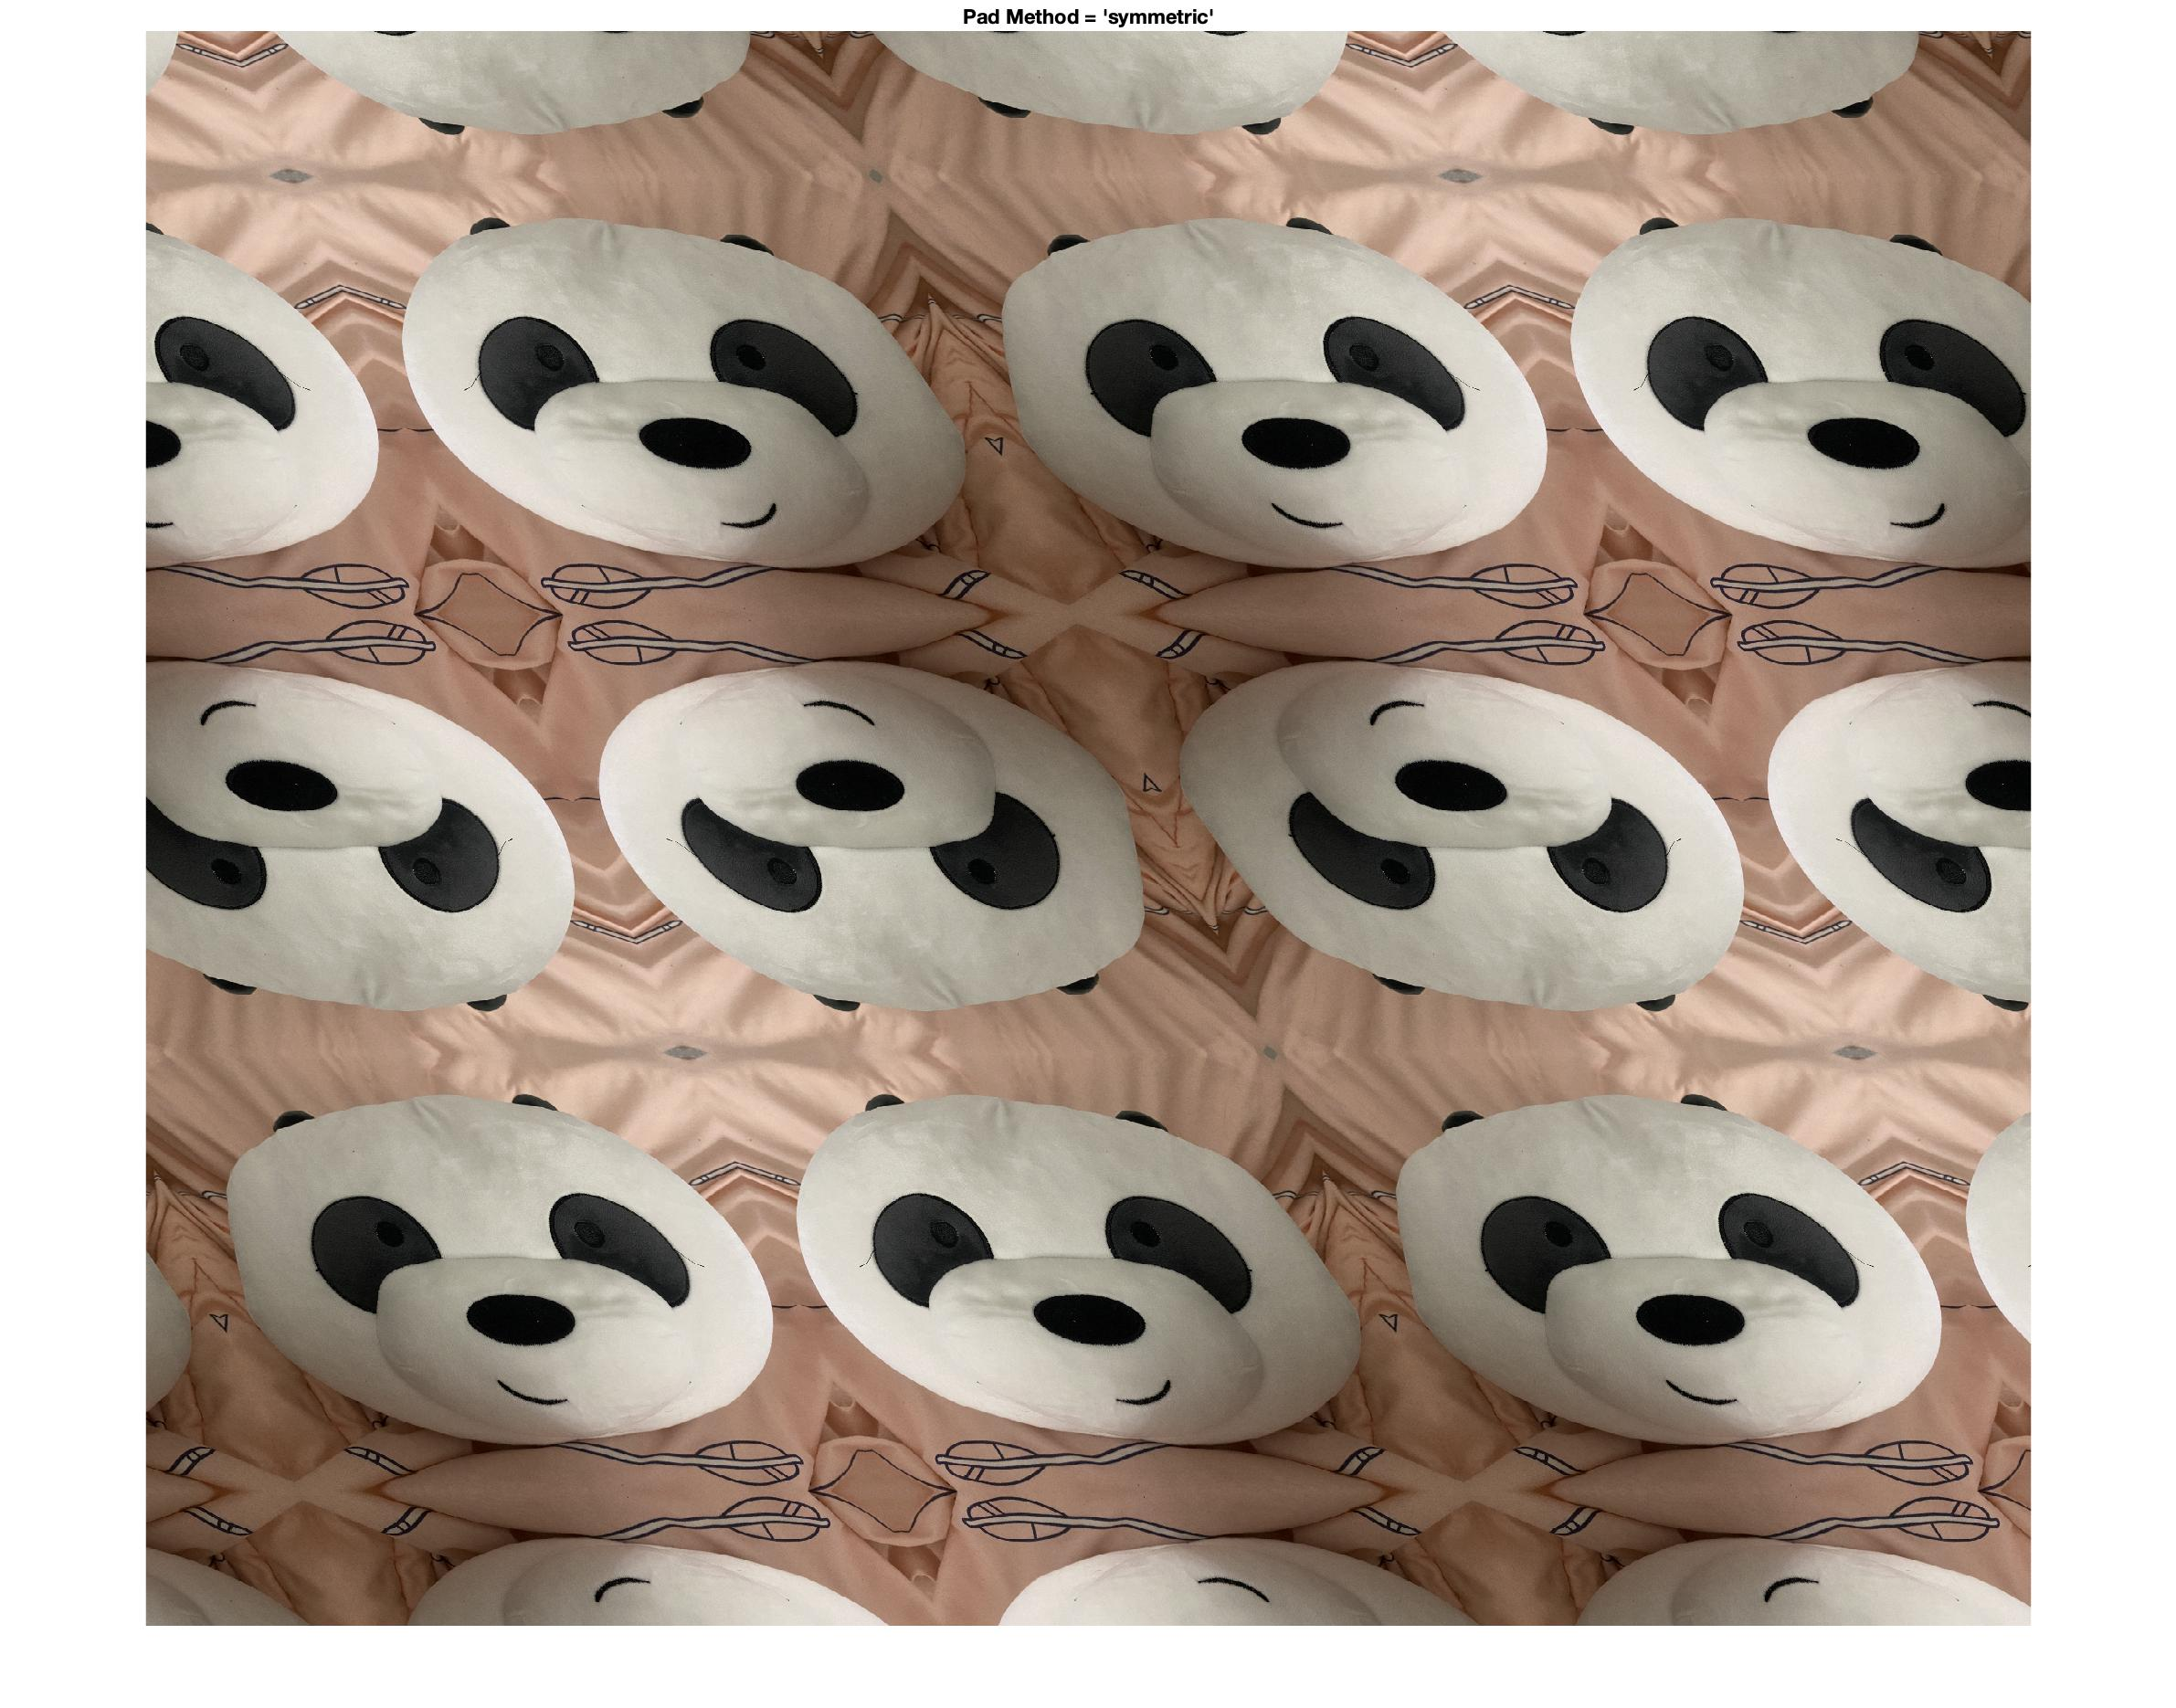
\includegraphics[width=0.8\linewidth]{images/img37.jpg}
\caption{Pad Method = ''symmetric''}
\label{fig:symmetric}
\end{figure}

\end{document}
